\documentclass[5p,times,twocolumn]{elsarticle}

\usepackage[utf8]{inputenc}

\usepackage{amsmath}
\usepackage{amssymb}
\usepackage{gensymb}
\usepackage{soul}
\usepackage{enumerate}
\usepackage{graphicx}% Include figure files
\usepackage{dcolumn}% Align table columns on decimal pion\index{\footnote{}}t
\usepackage{bm}% bold math
\usepackage{color}% bold math
\usepackage{hyperref}
\usepackage{epstopdf}
\usepackage{subcaption}
\usepackage{url}
\hyphenpenalty=1500
\exhyphenpenalty=1500

\title{The CLAS12 RICH Detector}
%\author{ }
%\date{November 2019}

\journal{Nuclear Instruments and Methods A}

\def\etal{{\it et al.}}
\def\MaPMT{MaPMT }
\def\MaPMTs{MaPMTs }
\def\MAROC{MAROC3 }
\def\dT{$\Delta T$ }
\makeindex
\begin{document}

\begin{frontmatter}

\author[a]{M.~Contalbrigo}
\author[f]{V.~Kubarovsky}
\author[b]{M.~Mirazita}
\author[f,b]{P.~Rossi}
\author[h]{E.~Aaron}
\author[b,j]{G.~Angelini}
\author[f]{H.~Avakian}
\author[a]{I.~Balossino}
\author[a]{L.~Barion}
\author[g]{K.~Bailey}
\author[h]{F.~Benmokhtar}
\author[h]{M.~Benninghoff}
\author[k]{W.~Brooks}
\author[c]{E.~Cisbani}
\author[f]{C.~Cuevas}
\author[f]{P.~Degtiarenko}
\author[f]{C.~Dickover}
\author[h]{J.~Goodwill}
\author[f]{G.~Jacobs}
\author[i]{K.~Joo}
\author[i]{A.~Kim}
\author[f]{T.~Lemon}
\author[b]{V.~Lucherini}
\author[a]{R.~Malaguti}
\author[f]{M.~McMullen}
\author[a]{A.~Movsisyan}
\author[d]{P.~Musico}
\author[g]{T.~O'Connor}
\author[b]{D.~Orecchini}
\author[e]{R.~Perrino}
\author[f]{B.~Raydo}
\author[b]{S.~Tomassini}
\author[a,b]{M.~Turisini}
\author[f]{A.~Yegneswaran}


\address[a]{INFN Sezione di Ferrara and University of Ferrara, Italy}
\address[b]{INFN Laboratori Nazionali di Frascati, Italy}
\address[c]{INFN Sezione di Roma1 - Gruppo Collegato Sanit\`a and Italian National Institute of Health, RM, Italy}
\address[d]{INFN Sezione di Genova, GE, Italy}
\address[e]{INFN Sezione di Bari, Italy}
\address[f]{Thomas Jefferson National Accelerator Facility, VA, USA}
\address[g]{Argonne National Laboratory, IL, USA}
\address[h]{Duquesne University, PA, USA}
\address[i]{University of Connecticut, CT, USA}
\address[j]{George Washington University, DC, USA}
\address[k]{Universidad Tecnica Federico Santa Maria, Valparaiso, Chile}

\begin{abstract}
  A Ring Imaging Cherenkov detector has been installed in the CLAS12 spectrometer at Jefferson Laboratory (JLab)
  to provide kaon identification in the momentum range between 3 and 8~GeV. The detector adopts a hybrid optics
  solution with aerogel radiator, light planar and spherical mirrors, and highly segmented photon detectors. We report
  here on the design, construction, and initial performance of the RICH during the commissioning of the detector and
  the first physics data taking period. 
\end{abstract}

\begin{keyword}
Ring-imaging Cherenkov detectors
\sep
PID detectors
\sep
Single-photon detection
\end{keyword}

%\maketitle

\end{frontmatter}

\begin{figure}[th]
\begin{center}
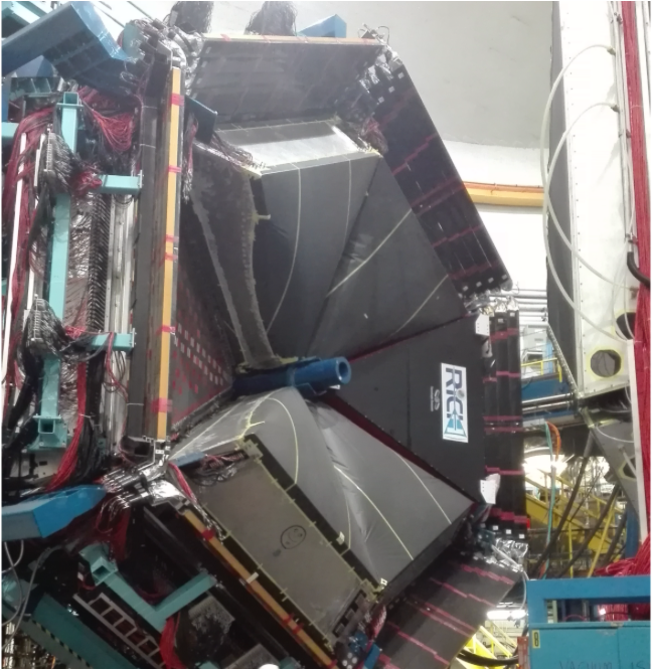
\includegraphics[width=0.80\columnwidth]{RICH_Installed.pdf}
\end{center}
\caption{The first module of the CLAS12 RICH installed in sector 4 of the Hall~B Forward Carriage.}
\label{Fig:RICHPic}
\end{figure}

%-----------------------------------------------
\section{Overview}
%-----------------------------------------------

Particle identification (PID) of hadrons in the original baseline design of the Forward Detector of CLAS12 is obtained
by combining the information from the High Threshold Cherenkov Counter (HTCC)~\cite{REF:htcc-nim}, Low Threshold
Cherenkov Counter (LTCC)~\cite{REF:ltcc-nim}, and Forward Time-of-Flight (FTOF)~\cite{REF:ftof-nim} systems. However,
no sufficient separation of kaons from pions and protons can be achieved by using only these detectors in the
momentum range relevant for the approved semi-inclusive deep inelastic scattering (SIDIS) physics program,
i.e. between 3 and 8~GeV. Therefore, improved particle identification in this momentum range is achieved by
replacing two sectors of the existing LTCC with Ring Imaging Cherenkov (RICH) detectors. The first module of the
RICH detector was completed before the start of the physics run, see Fig.~\ref{Fig:RICHPic}, while the installation
of the second module in the opposite sector is foreseen for the beginning of the CLAS12 operation with polarized
targets. This article reports on the design, construction, and initial performance of the first RICH module. The second
module will be identical to the first one.

The idea of a RICH detector is based on the fact that when a fast particle crosses a radiator with a velocity $\beta$
larger than the velocity of the light in that medium, it emits Cherenkov photons. The light is emitted in a cone with
opening angle $\theta_C$ given by $\cos(\theta_C)=[\beta n(\lambda)]^{-1}$, where $n(\lambda)$ is the refractive index
of the radiator, which may depend on the wavelength $\lambda$. After a gap region where the cone opens up, the
photons are detected and the ring can be reconstructed. A precision measurement of the Cherenkov angle provides
the velocity of the particle and, together with information from the tracking system, it allows its identification. Thus,
the capability of identify particles with a known momentum and different velocity is governed by the Cherenkov angle
resolution, and it can be effectively parameterized by the separation in units of resolution $n_{\sigma}$ between the
angle distributions for the various particles.

%-----------------------------------------------
\section{Detector Requirements}
%-----------------------------------------------

The CLAS12 spectrometer in Hall~B~\cite{REF:overview-nim} is designed to operate with highly polarized beams and
nucleon targets at a luminosity of $10^{35}$~cm$^{-2}$s$^{-1}$. Under these conditions the production rate of protons,
kaons, and pions studied using SIDIS Monte Carlo event-lists is such that, in most of the kinematic plane, the kaon rate
is about one order of magnitude lower than the rate of pions and protons. Thus, successful kaon identification requires
a rejection factor from pions around 1:500, i.e. a contamination in the kaon sample of a few percent. This corresponds to
4$\sigma$ separation. In the momentum range between 3 and 8~GeV, neither gas nor liquid radiators provide sufficient
angular separation to achieve the required pion rejection factor (see Fig.~\ref{Fig:Radiators}) and the only viable
solution is silica aerogel, an amorphous solid network of $\rm SiO_2$ nanocrystals with a very low macroscopic density
and a refractive index in between gases and liquids.

To detect the Cherenkov light emitted in the visible wavelength
range, Hamamatsu Multi-Anode PhotoMultipliers Tubes (MaPMTs) were chosen for their high quantum efficiency in the
visible and near ultraviolet (UV) regions, their fast response, and the required spatial resolution. Since the RICH
detector must fit into the original CLAS12 Forward Carriage, there were several constraints imposed upon its design.
Each sector required a projective geometry, limited depth of 1.2~m, and $\sim$4.5~m$^2$ entrance windows.
Simulation studies favored a hybrid imaging Cherenkov detector design incorporating aerogel radiators, visible light
photon detectors, and a focusing mirror system. The focusing mirror system is used to reduce the detection area
instrumented by the photon detectors to $\sim$1~m$^2$ per sector, minimizing costs and influence on the Forward
Time-of-Flight and electromagnetic calorimeter~\cite{REF:ecal-nim} systems. Depending upon the incident particle track
angle, Cherenkov light is either imaged directly or after one or more reflections and passes through the aerogel.
Figure~\ref{Fig:RICHsketch} shows a schematic view of two examples of direct imaging and imaging after multiple
reflections. Such a peculiar hybrid-optics design is an innovative solution that has been successfully validated with 
a test-beam campaign~\cite{REF:RICH2013}. 

\begin{figure}
\begin{center}
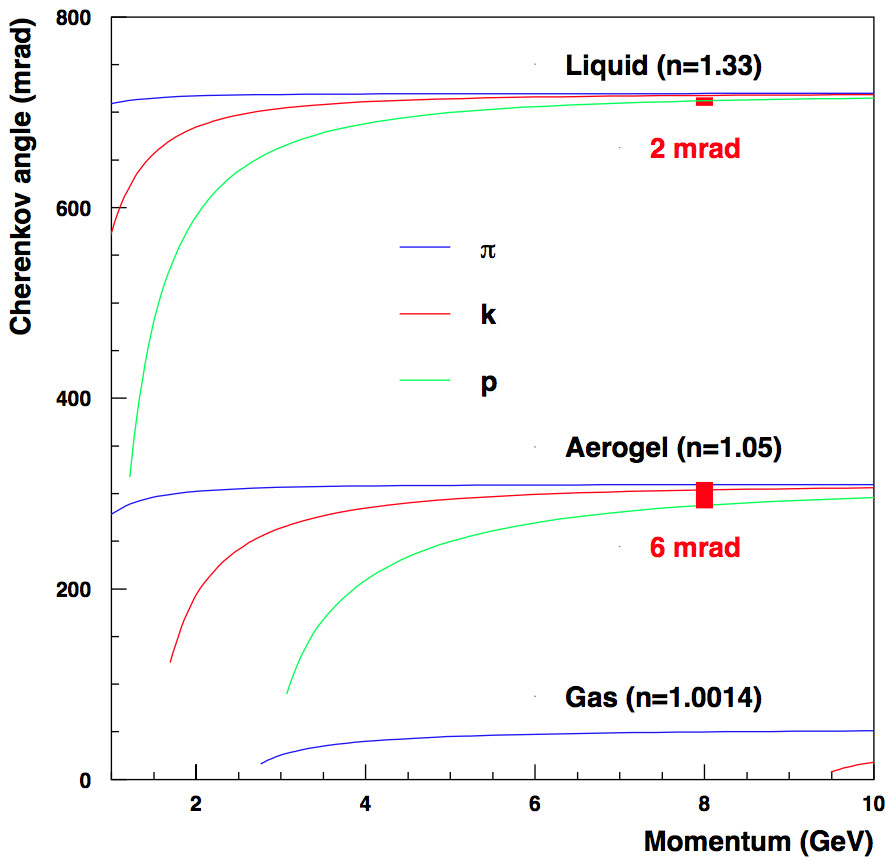
\includegraphics[width=0.45\textwidth]{radiators.png}
\caption{Cherenkov light opening angle as a function of the momentum for different particles using liquid, gas, or
  aerogel radiators. The angular separation between kaons and pions at the highest momenta is also indicated.}
\label{Fig:Radiators}
\end{center}
\end{figure}

\begin{figure}
\begin{center}
%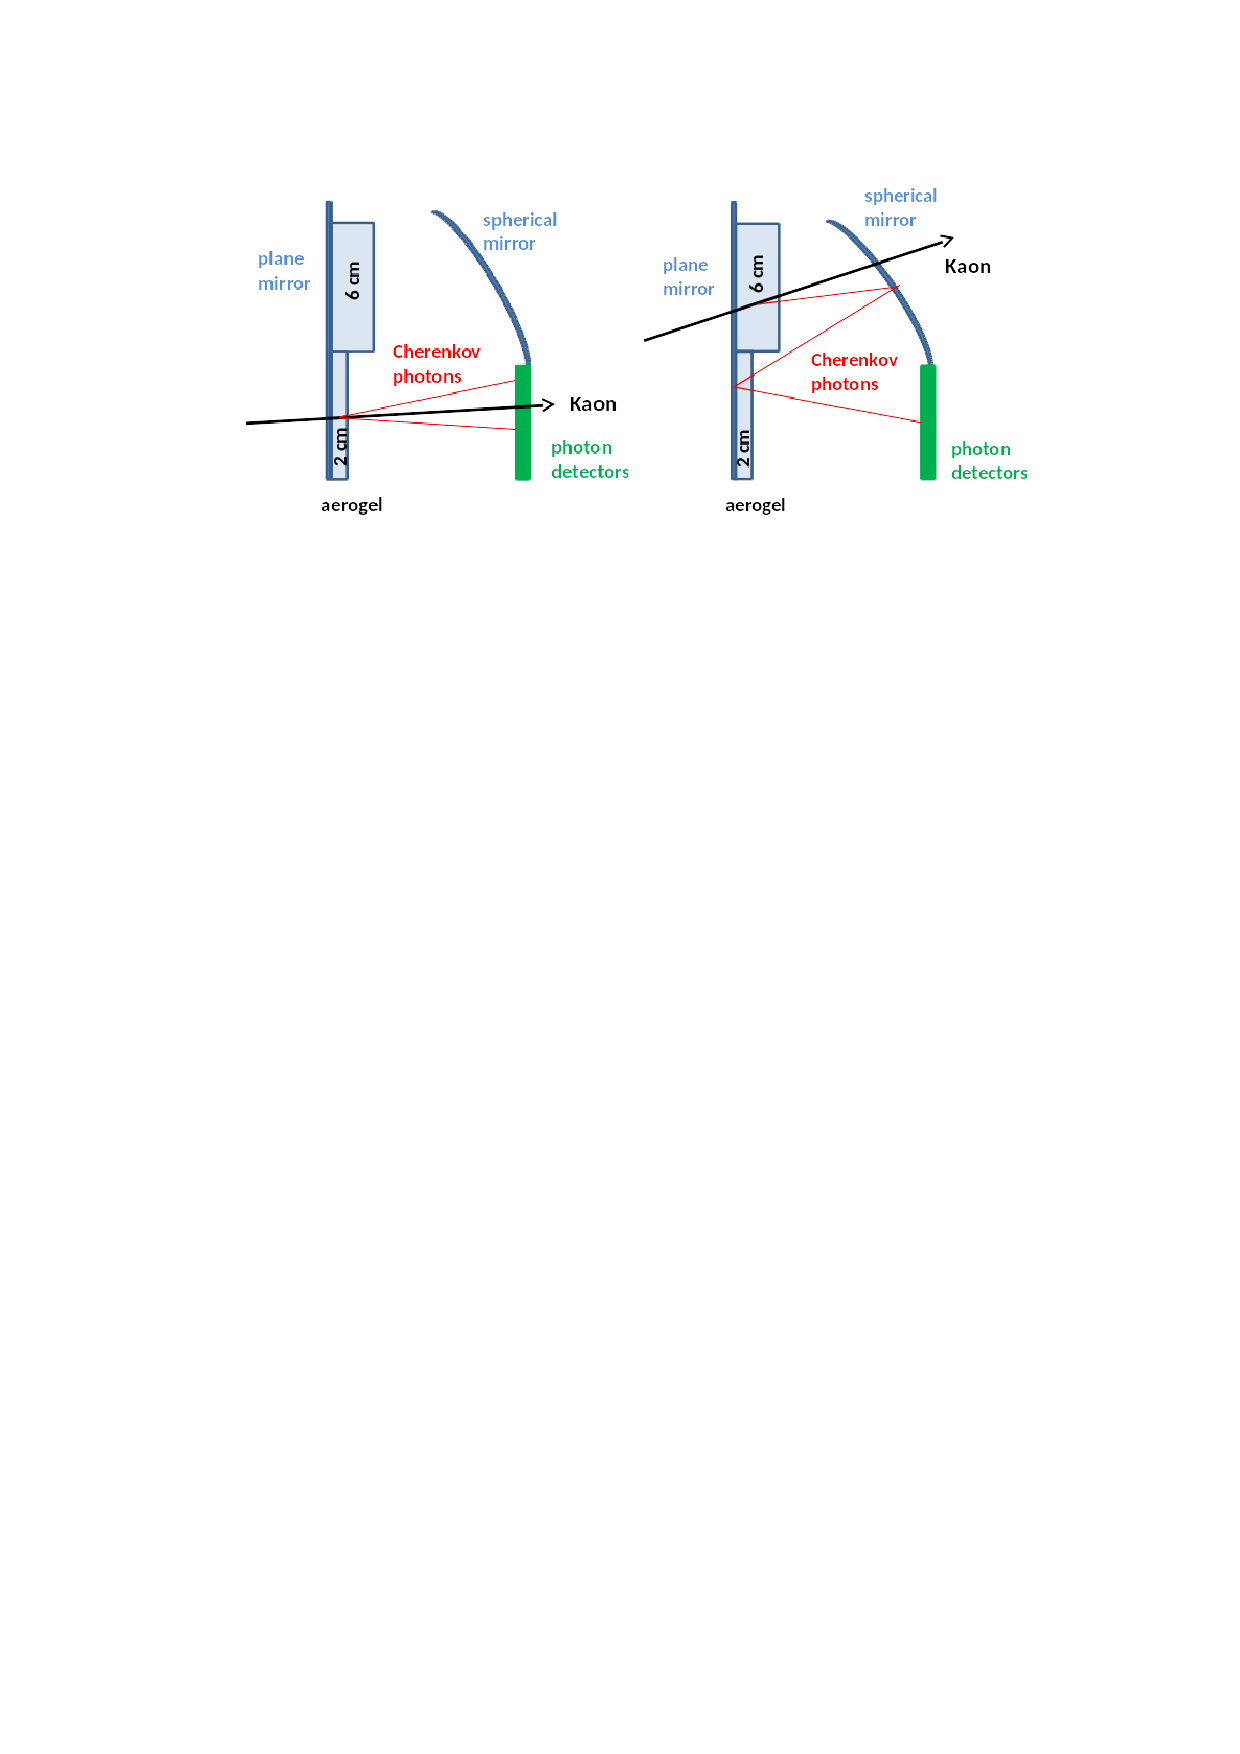
\includegraphics[width=0.50\textwidth]{Layout.pdf}
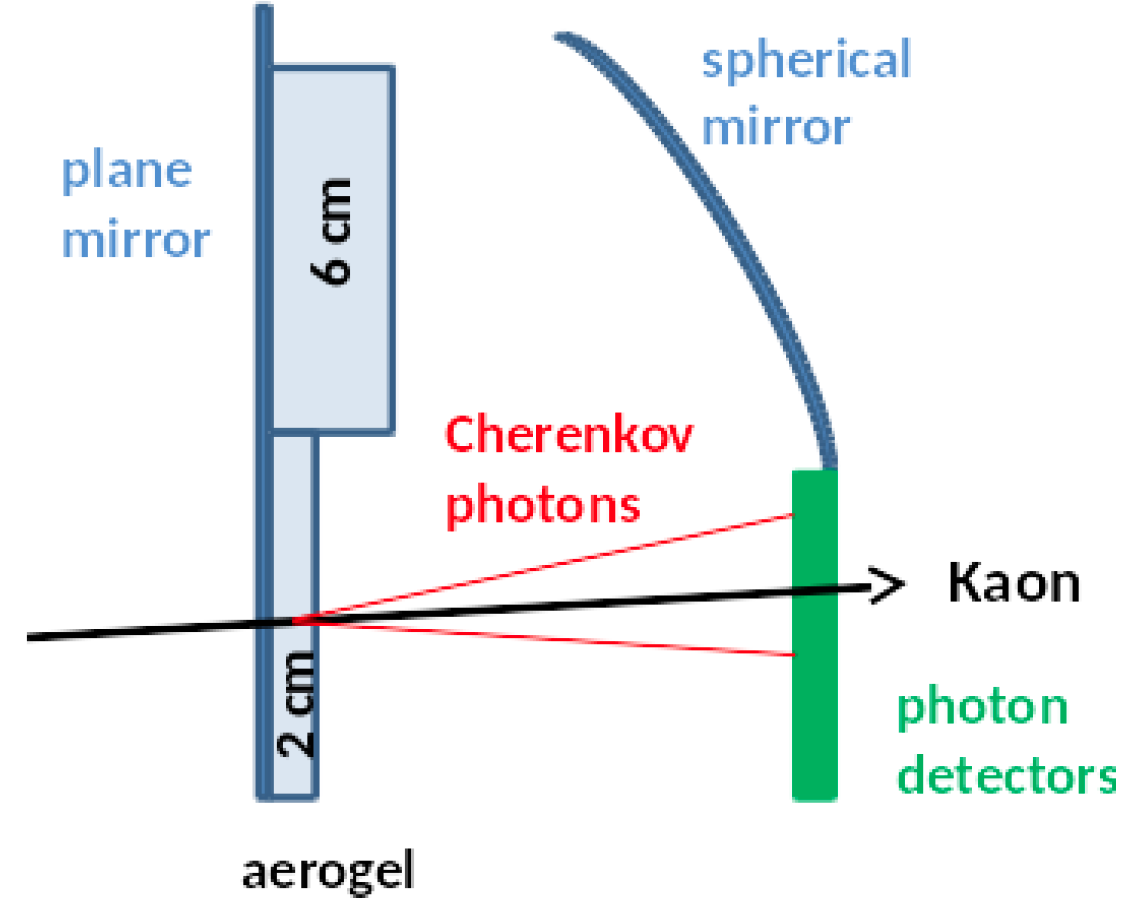
\includegraphics[width=0.38\textwidth]{Layout_direct.png}
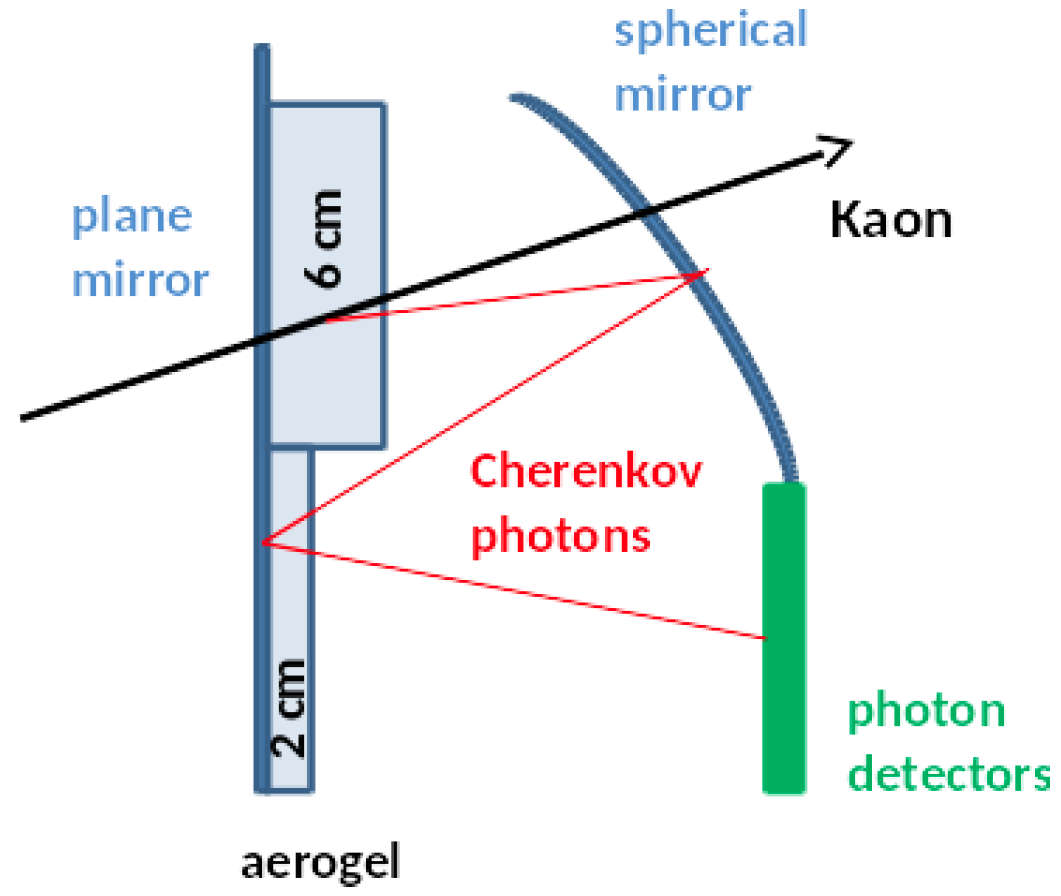
\includegraphics[width=0.38\textwidth]{Layout_reflect.png}
\caption{Examples of CLAS12 RICH imaging: direct detection of the Cherenkov cone produced in the thin aerogel layer
  (top plot); detection of the Cherenkov cone produced in the thick aerogel layer after multiple reflections and passes
  through the thin aerogel layer (bottom plot).}
\label{Fig:RICHsketch}
\end{center}
\end{figure}

%-----------------------------------------------
\section{Detector Design}
%-----------------------------------------------

The RICH detector replaces two sectors of the existing gas Low Threshold Cherenkov detector (LTCC), which is located
at a 5~m distance from the beam-target interaction point. The first RICH module was designed while the CLAS12 spectrometer was
already under construction and,  as a consequence, it had to cover the same large area to match the trapezoidal shape of
the LTCC sector. This resulted in several challenging requirements for the mechanical structure. The guiding principles
were to minimize the material budget inside the acceptance and to limit the impact on the downstream detectors,
ensuring at the same time the rigidity of the structure imposed by the optical requirements. Therefore, light materials,
in particular carbon fiber, were largely utilized for all elements inside the CLAS12 acceptance. For all the parts with
large dimensions, the sandwich technique, in which two thin solid skins are glued together on a thick honeycomb core, was
also used. This technique indeed combines high stiffness with substantial weight reduction, resulting in a total weight of
the detector of about 900~kg, $\sim$30\% lower than the LTCC.

A sketch of the detector is shown in Fig.~\ref{Fig:RICHexplo}. It is composed of a trapezoidal box (larger base of
4.2~m, smaller base of 0.3~m, height of 3.7~m, and depth of 1.2~m) in which all of the active elements are installed:
the wall of aerogel tiles, the mirrors, the photomultiplier tubes (PMTs), and the electronics. The main structural elements of
the box are: the two lateral panels made of aluminum sandwich, the top panel made of carbon fiber sandwich, and the
two upper angular elements and the bottom element made of aluminum. Each of the lateral panels supports two planar
mirrors, while another planar mirror is installed on the bottom of the box. The box is closed on the front face (with
respect to the beam direction) by two entrance panels made of a sandwich of two 1-mm-thick carbon fiber skins glued on a
Nomex honeycomb core. Two planar mirrors with a wall of 2-cm-thick aerogel tiles are installed on the lower entrance panel, while
a wall made of two layers of 3-cm-thick aerogel tiles is installed on the upper one. Therefore, the profile of the entrance panels
was specifically designed not only to ensure the best light and gas tightness, but also to include stiffening ribs for
the installation of the mirrors and the aerogel. The same sandwich structure was used for the electronics panel, located
on the bottom part of the backward face of the box. It is composed of a main panel where all of the front-end electronics
and the PMTs are installed, and a thin cover. The panel and the cover are screwed together on the mechanical
structure, making a very rigid system. Finally, a very light exit panel made of a thin Tedlar sheet glued on an aluminum
frame not supporting any active element, closes the back face of the trapezoidal box. 

The total material budget of the detector is largely dominated by the electronics panel, which contributes to
approximately 0.3 $X_0$ in the region from the beamline up to about 17$^\circ$. A sizable contribution comes also
from the aerogel (with a maximum contribution of 0.05 $X_0$ in the polar angles from 17$^\circ$ to 26$^\circ$),
while other active components like the spherical and planar mirrors contribute only $\approx$0.01 $X_0$ each.
The total material budget of the passive elements is estimated to be, on average, below 0.05 $X_0$.

The mechanical structures and all of the active elements (mirrors, aerogel, electronics, MaPMTs) define the RICH
detector. The RICH is attached to the CLAS12 Forward Carriage by means of steel connections, attached to the
angular and bottom elements. Detailed Finite Element Analysis (FEA) studies were performed in order to optimize
the design of the detector with respect to the maximum deformation allowed by the required accuracy of the optical
systems. These studies included optimization of the ratio between the skin and honeycomb thicknesses of the sandwich,
and of the total thickness and profile of various stiffening and connection elements. Simulations of the load conditions
during the assembly and installation of the detector and in the RICH final position in CLAS12 were also performed
together with a seismic analysis \footnote{According to US regulations, seismic analyses are performed by increasing
the expected weight load by 10\%.}. These simulations demonstrated that all stresses produced on the detector
elements during the installation are well inside the elastic regime, and that the total deformations expected when the
RICH is installed in CLAS12 never exceed a few mm.

\begin{figure}
\begin{center}
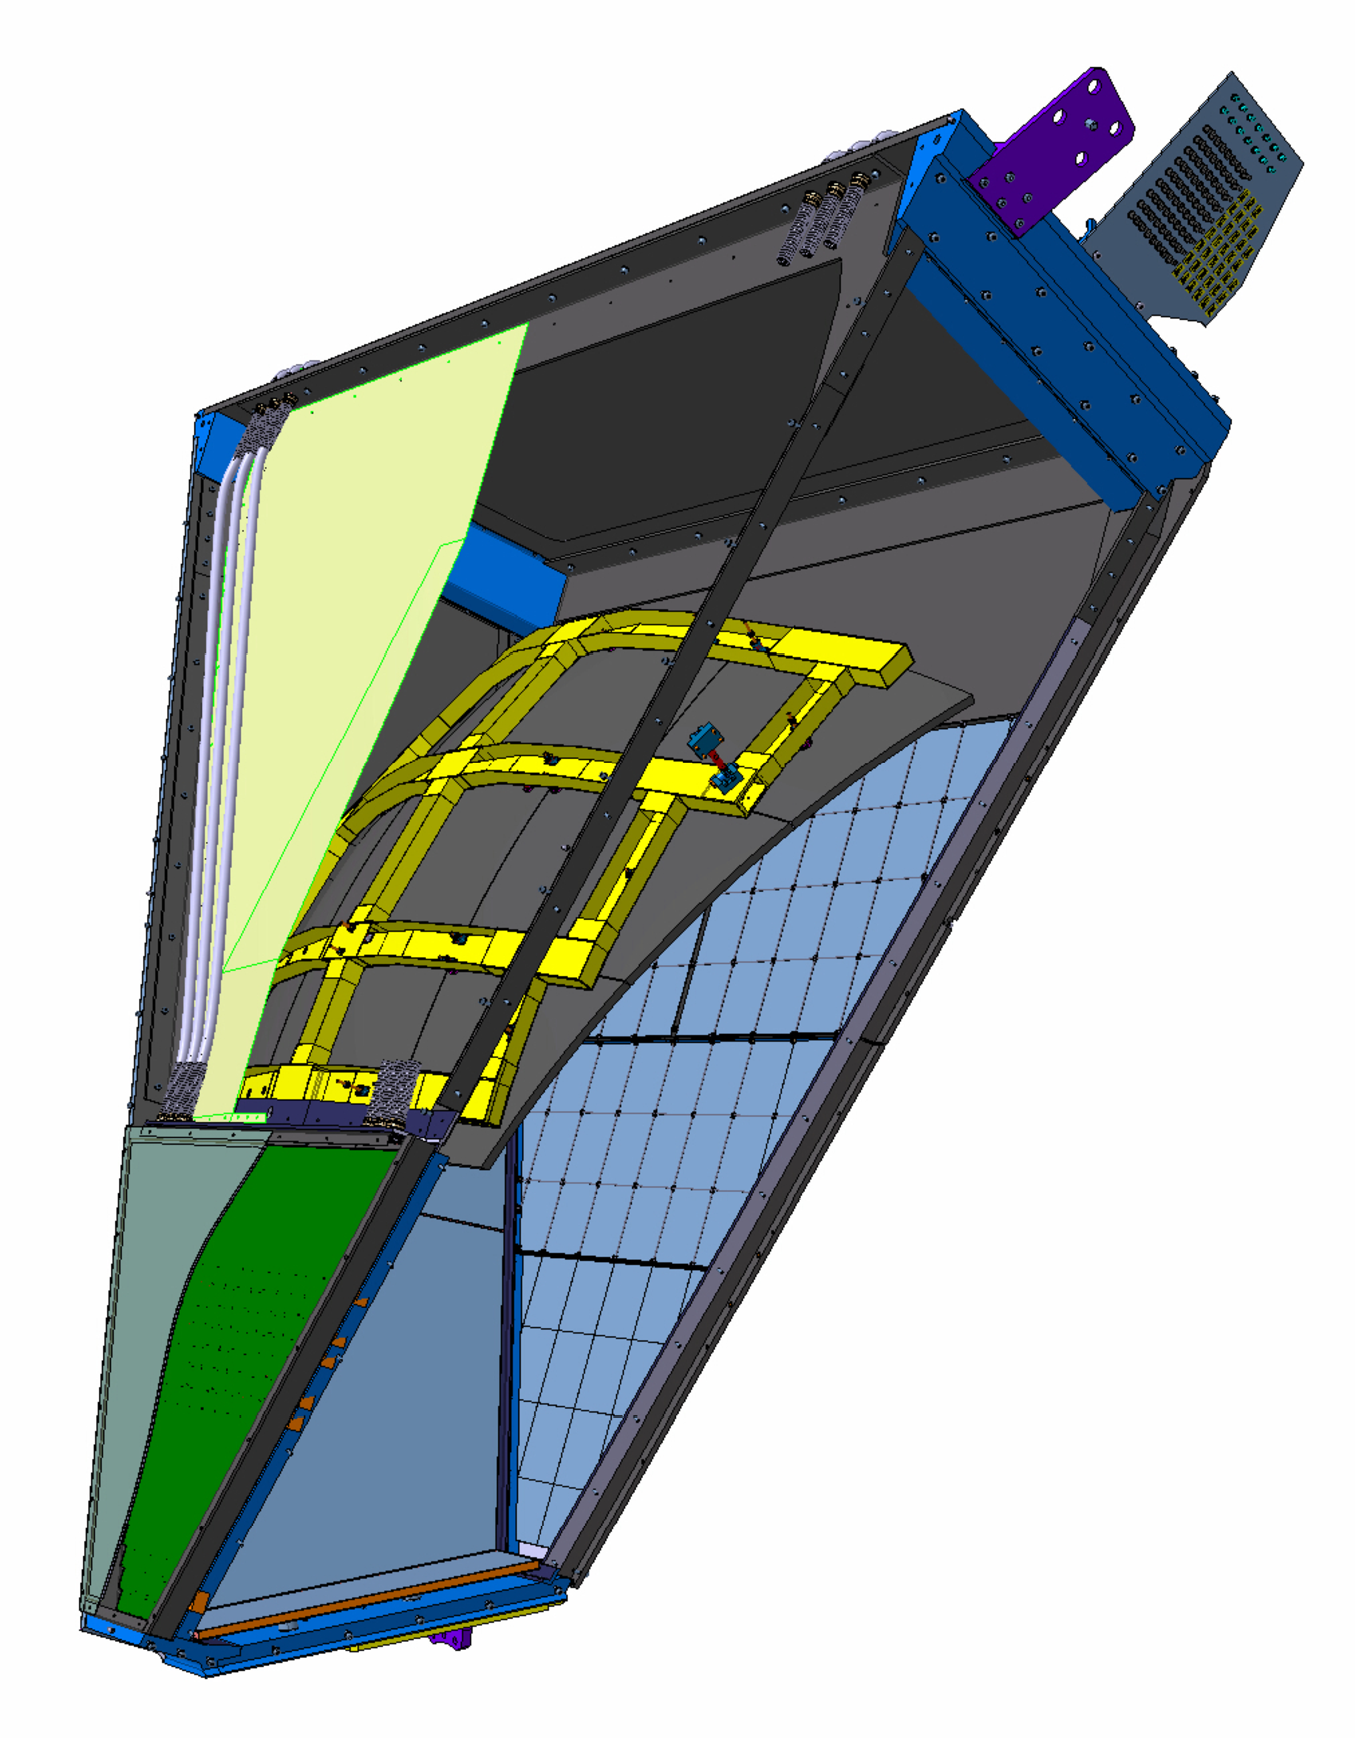
\includegraphics[width=0.45\textwidth]{RICH.pdf}
\caption{A schematic drawing of the CLAS12 RICH with the internal components highlighted. From left to right, the 
components of the upper half are exit panel, spherical mirror support and sub-mirrors, double 3-cm-thick aerogel
layer, and entrance panel. The components of the lower half are cover, electronics panel - mounting the front-end readout
and the \MaPMT sensors, 2-cm-thick aerogel layer, front planar mirrors, and entrance panel.}
\label{Fig:RICHexplo}
\end{center}
\end{figure}

%The total material budget of the detector is largely dominated by the electronic panel, which contributes to approximately 0.3 $X_0$ in the region from the beam line up to about 17$^\circ$. A sizeable contribution comes also from the aerogel (maximum 0.05 $X_0$ in the polar angles from 17$^\circ$ to 26$^\circ$), while other active components like the spherical and planar mirrors contributes only to approximately 0.01 $X_0$ each. The total material budget of the dead elements is estimated to be, on average, below 0.05 $X_0$.

%-----------------------------------------------
\section{The RICH Components}
%-----------------------------------------------

%-----------------------------------------------
\subsection{The Mirror System}
%-----------------------------------------------

The mirror system, composed of planar and spherical mirrors, was designed to minimize the photon loss and to direct
as much of the Cherenkov radiation as possible toward the photodetectors. Simulations were performed to optimize
the segmentation, the position and the radius of curvature of these mirrors, and to define the specifications of the
optical performance. A drawing of the system is shown in Fig.~\ref{Fig:RICHmirrors}.

\begin{figure}
\begin{center}
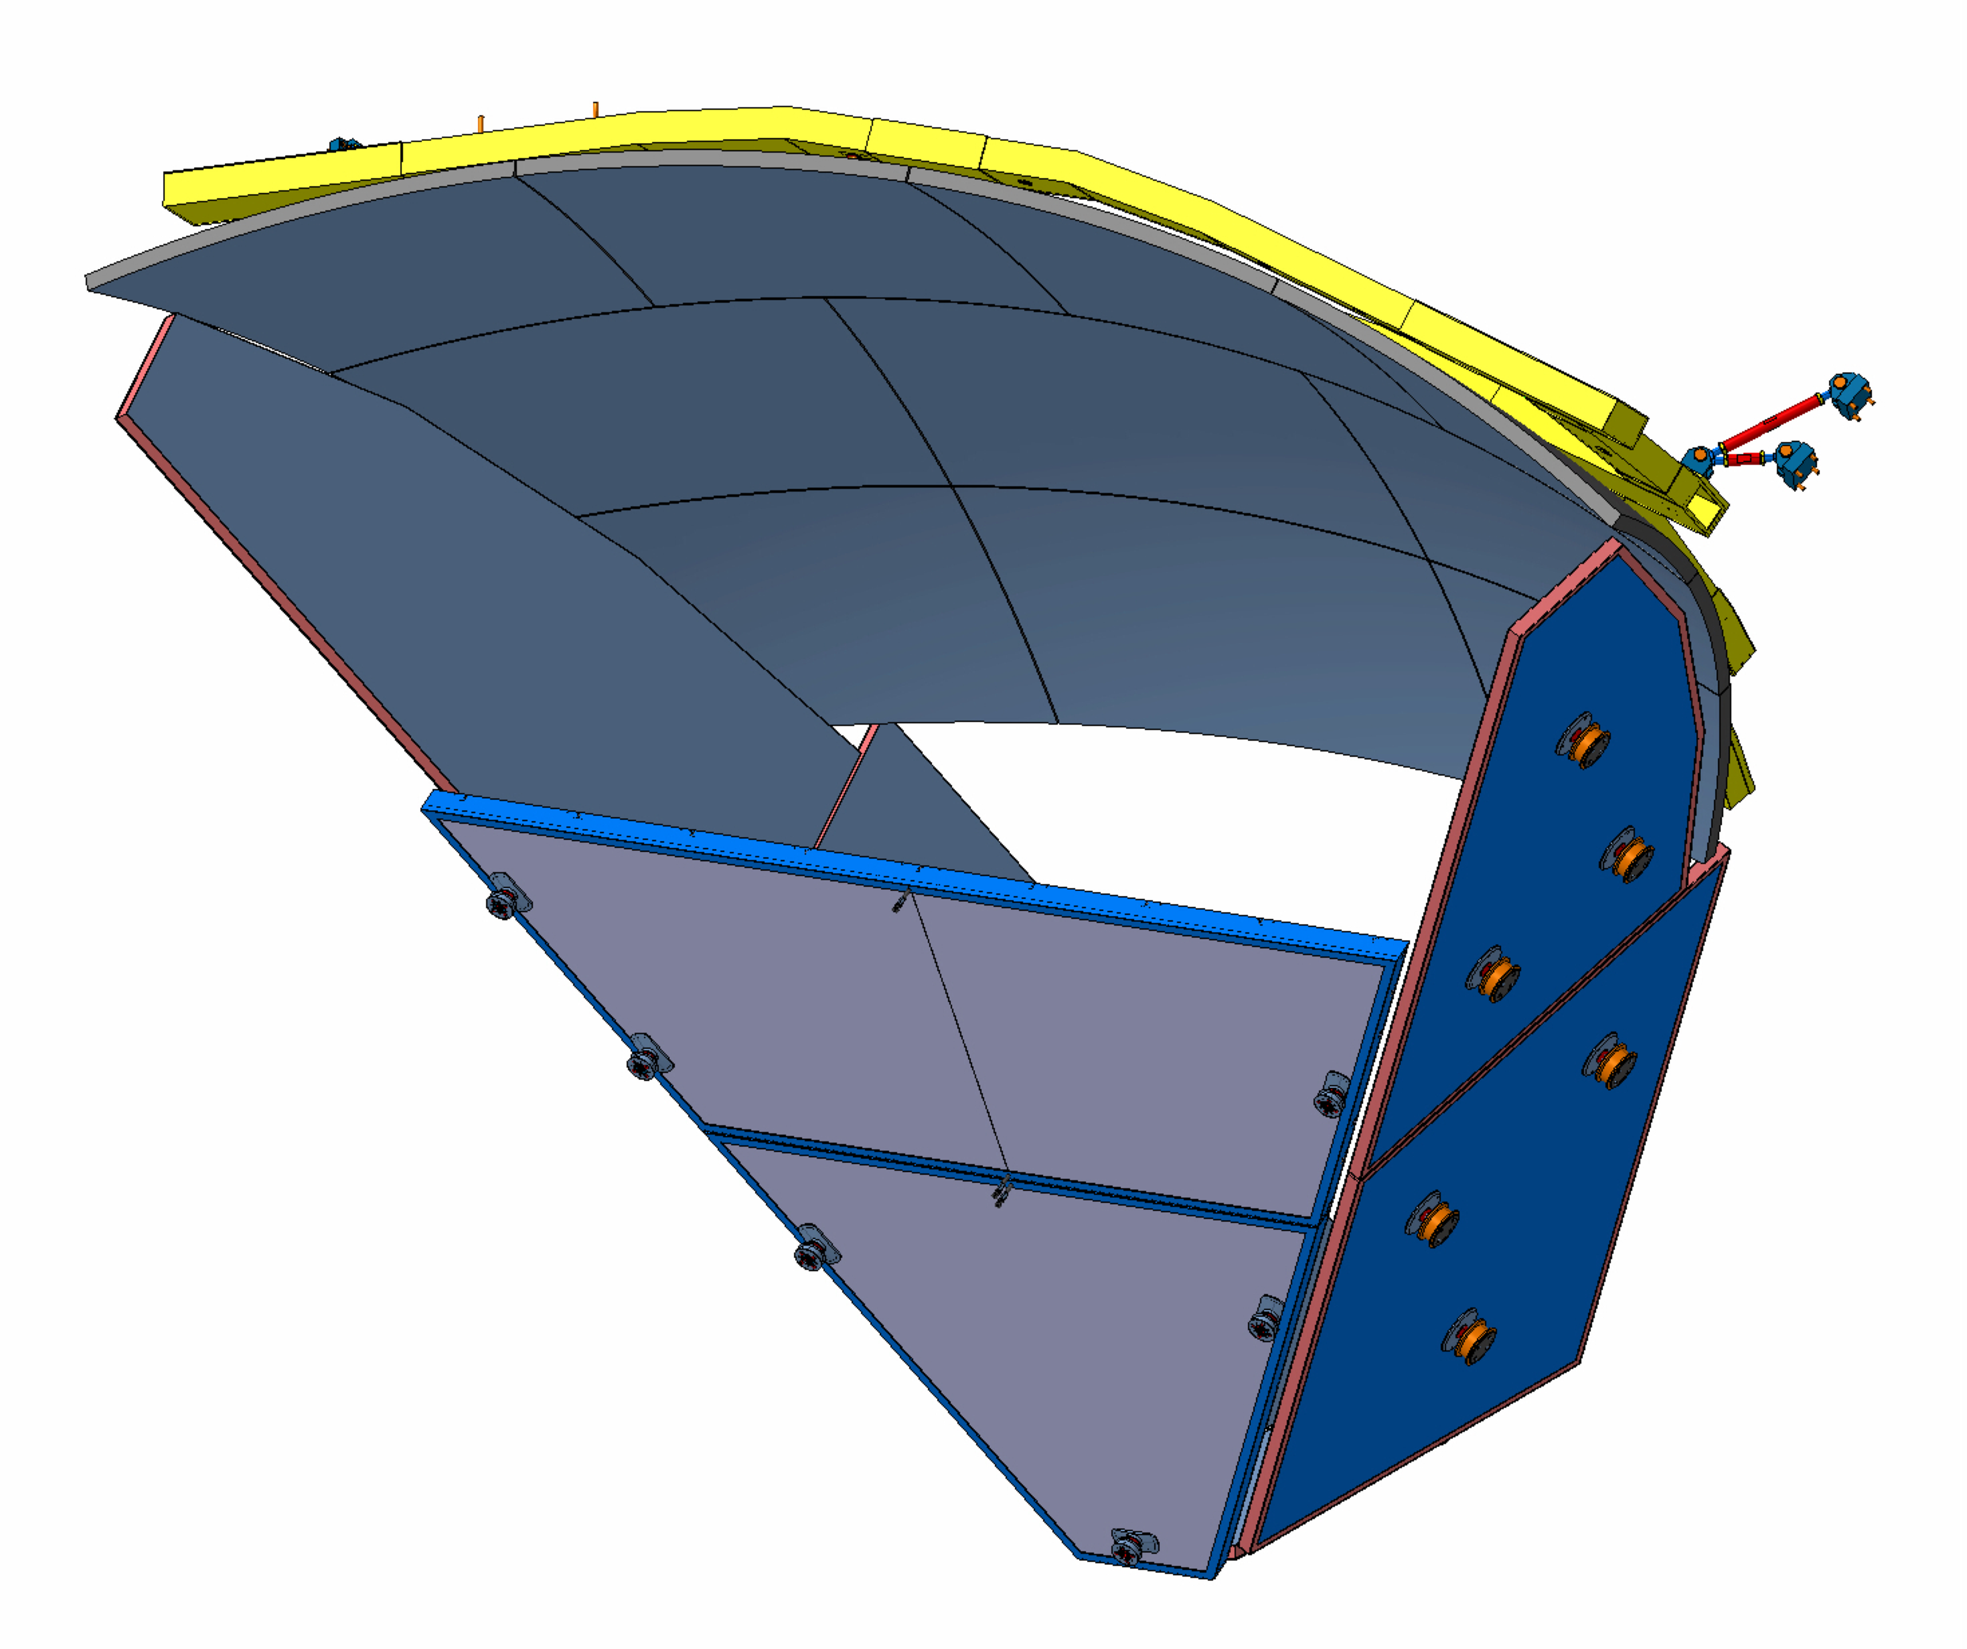
\includegraphics[width=0.50\textwidth]{RICHmirrors.pdf}
\caption{Drawing of the CLAS12 RICH mirror system with their mounting joints. The 10 sub-mirrors of the spherical mirror face the
two front planar mirrors. An array of planar mirrors, two in each side and one (not visible) on the 
bottom, completes the light containment system.}
\label{Fig:RICHmirrors}
\end{center}
\end{figure}

%-----------------------------------------------
\subsubsection{The Spherical Mirrors}
%-----------------------------------------------

The spherical mirror system, installed inside the box in front of the exit panel, has a total surface of about 3.6~m$^2$,
a radius of curvature $R= 2.7$~m, and is segmented into 10 sub-mirrors. They were produced by the {\it Composite
Mirror Applications} company~\cite{REF:CMA}, and are made of two layers of carbon fiber glued on a honeycomb
core of small carbon fiber cylinders. The areal weight of these mirrors is $\approx$5~kg/m$^2$, with an
improvement of about 10\% with respect to the mirrors produced by the same company for the LHCb experiment
\cite{REF:LHCbMirrors}. Each mirror is positioned on a light carbon frame by means of three special joints equipped
with a spring and a precision screw that allowed their relative alignment. The frame is then attached to the mechanical
structure by means of three similar joints that allow the alignment of the full mirror system with respect to the other
active elements of the detector.

The accuracy of the spherical surface of the sub-mirrors was quantified by means of a so-called spot size
measurement, in which each mirror was illuminated with a point-like light source and the size of the reflected spot
was measured by a XIMEA camera with a 1-cm-wide CMOS sensor. The size of the spot is quantified by $D_0$, which
is defined as the minimum diameter containing 90\% of the total reflected light, and is related to the angular resolution
of the reflected photons by the relation

\begin{equation}
  \sigma_{\theta} = \frac{D_0}{8 R}.
\end{equation}

The smaller $D_0$ is, the closer the mirror surface is to a perfect sphere. The measurements also allow for the
extraction of the radius of curvature, which corresponds to the distance between the camera and the mirror where
the spot size is minimal. The results of a typical measurement of one sub-mirror are shown in Fig.~\ref{Fig:SpotCMA},
where $D_0$ as a function of the distance and the shape of the spot at the beginning of the distance scan and
at the minimum are shown. All of the sub-mirrors exhibit a $D_0$ smaller than 1.5~mm, which means $\sigma_{\theta}$
significantly below 1~mrad, and a variation in the measured radii below 0.5\%. All of these numbers are well within the
specifications.

\begin{figure}
\begin{center}
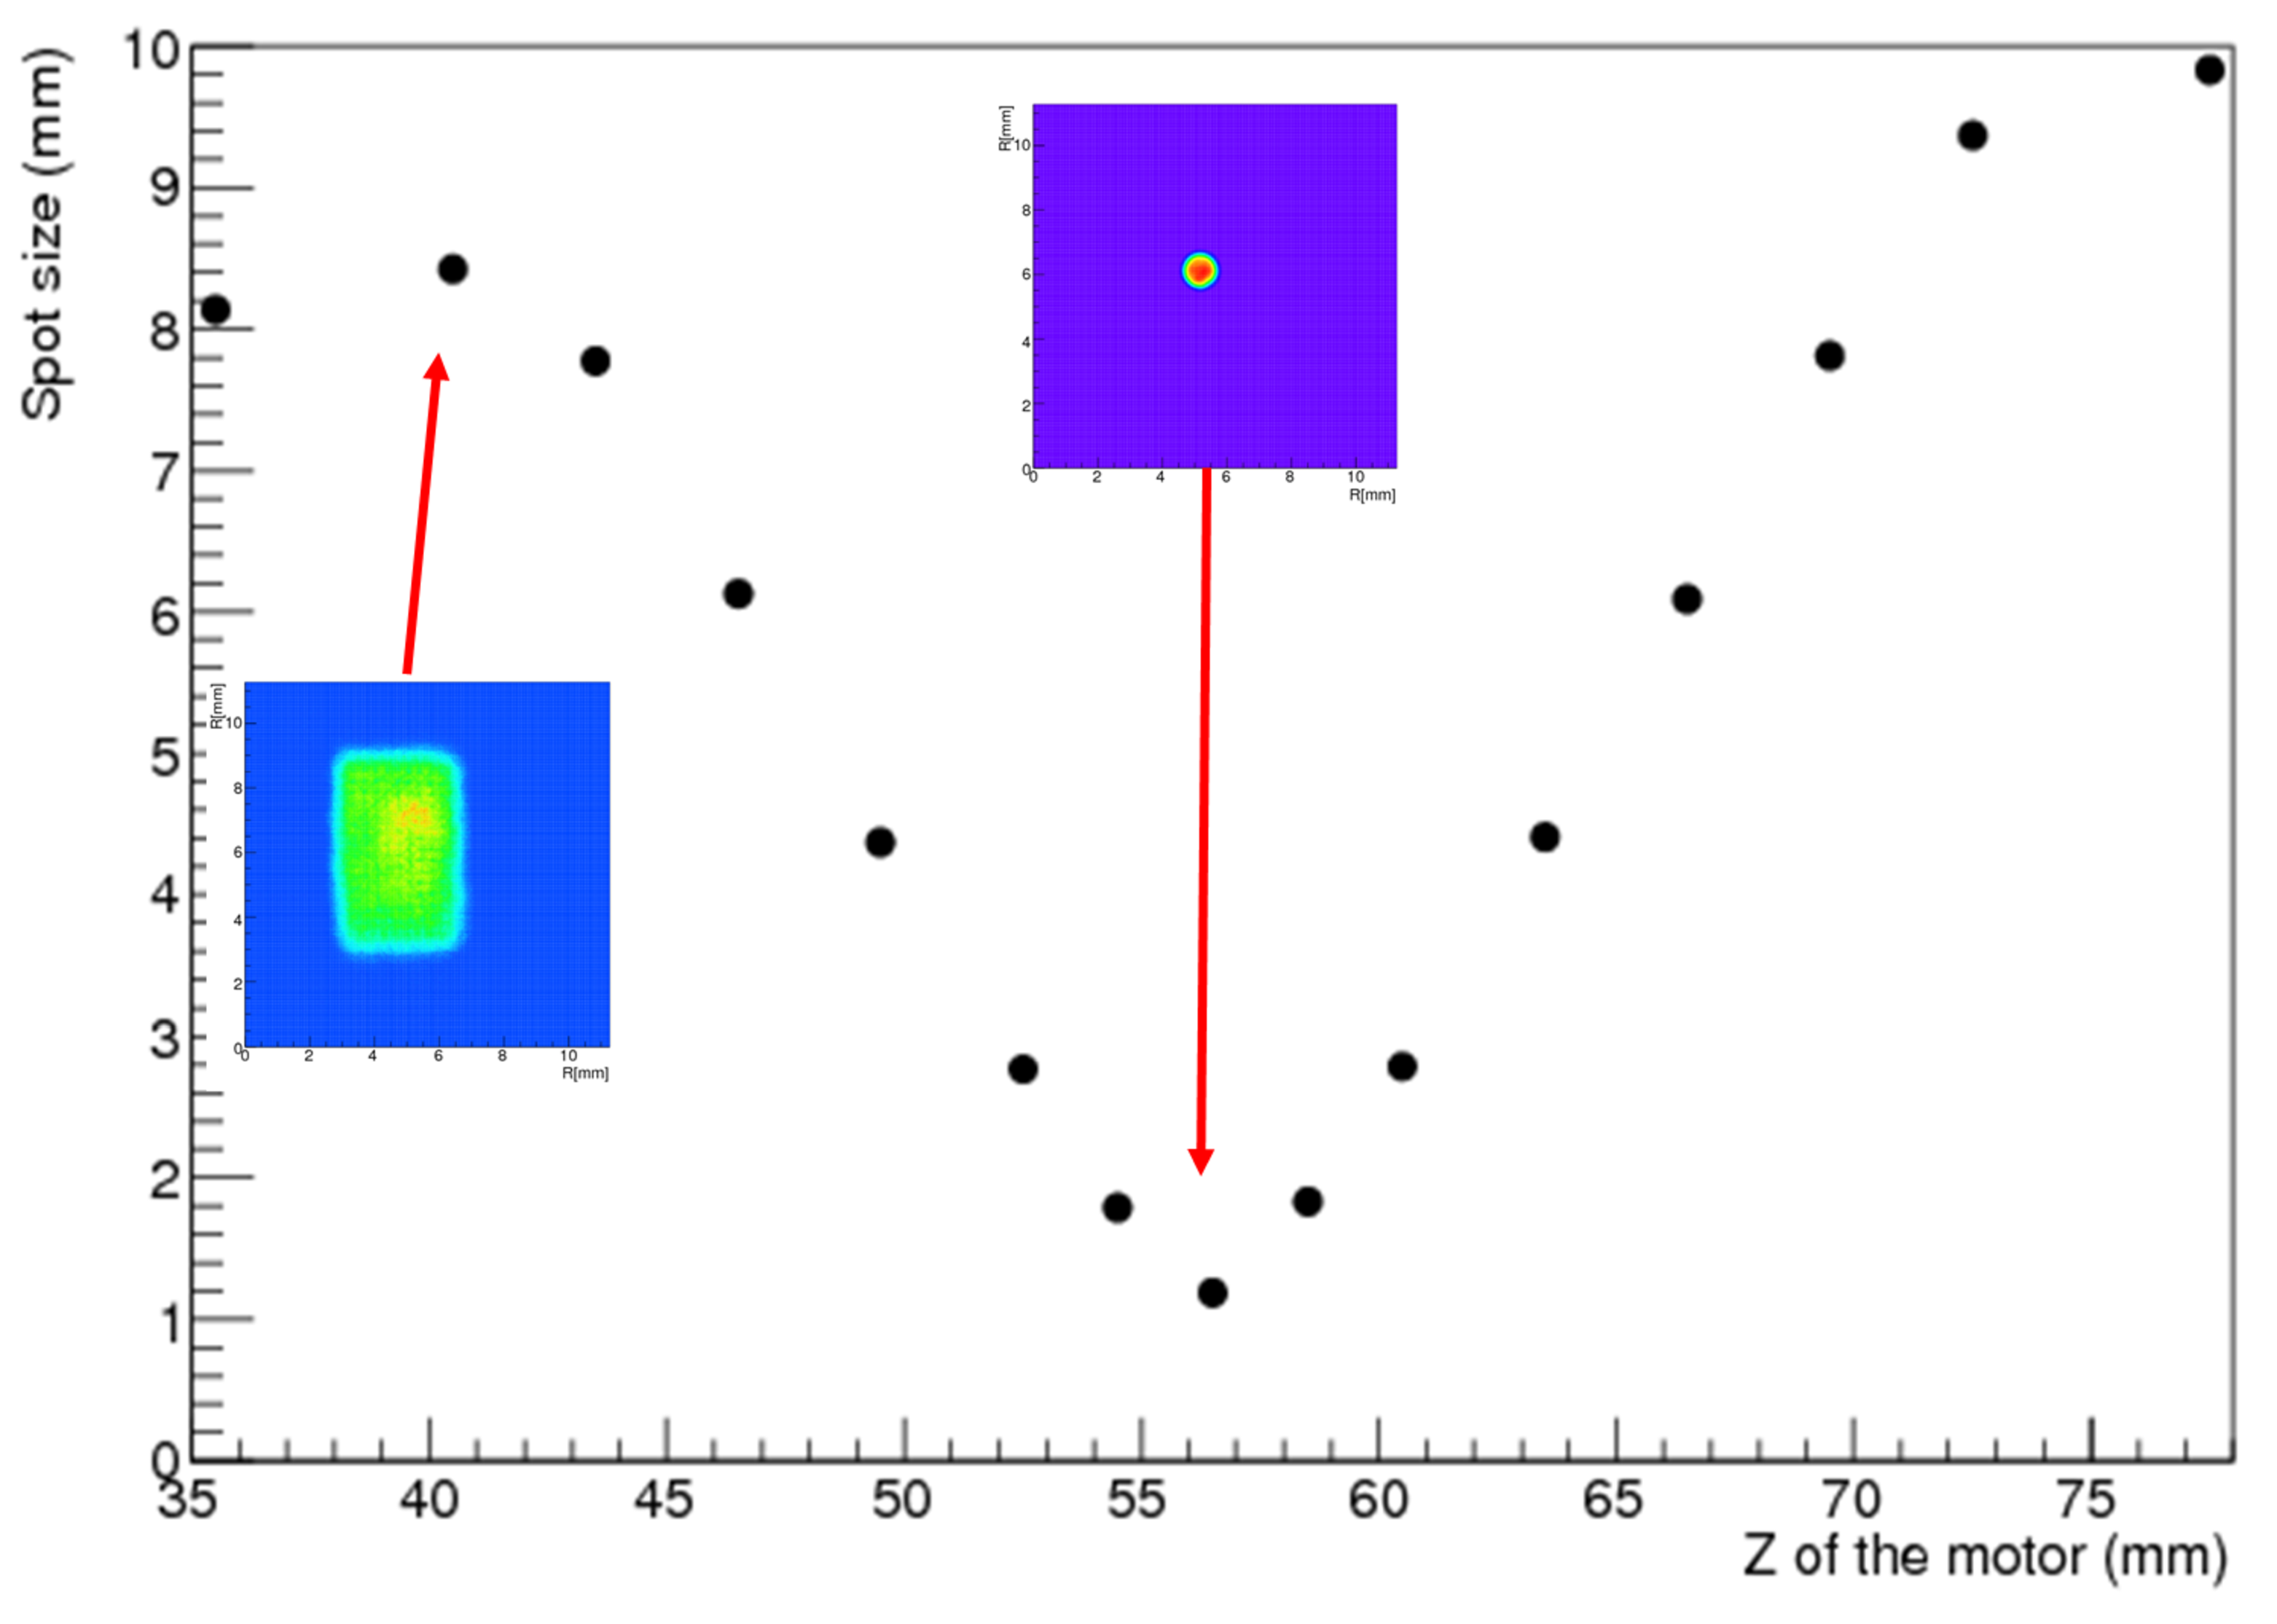
\includegraphics[width=0.45\textwidth]{SpotCMA.pdf}
\caption{$D_0$ as function of the distance between the mirror and the camera for one of the spherical sub-mirrors.
  The two inserts show the shape of the reflected spot at the beginning of the distance scan and at the minimum.}
\label{Fig:SpotCMA}
\end{center}
\end{figure}

The sub-mirrors were coated with a reflecting layer by {\it Evaporated Coatings Inc}~\cite{REF:ECI}. The quality of
this coating was verified by measuring the reflectivity on several surface spots in the wavelength range from 300 to
650~nm. For all of the sub-mirrors, we obtained on average a reflectivity between 88\% and 90\%, relatively flat over
the whole wavelength range.

%-----------------------------------------------
\subsubsection{The Planar Mirrors}
%-----------------------------------------------

The planar mirror system is composed of 7 mirrors: two installed on each of the lateral panels, two on the frontal panel,
and one on the bottom, for a total surface area of about 6.5~m$^2$. These mirrors were produced by the {\it Media
Lario} company~\cite{REF:MediaLario} and are made of two thin layers of glass glued on an aluminum honeycomb core.
This is a standard technique widely used in telescopes for astrophysics studies but used for the first time in nuclear
physics experiments, and allows for the production of mirrors as light as the carbon fiber ones but at much lower cost.
Being in the acceptance of the detector, the frontal mirrors use very thin (0.7~mm) glass layers, allowing a reduction of
the material budget down to about 0.01 $X_0$, while for the lateral and the bottom mirrors, thicker (1.6~mm) glass
layers were used.

The planarity of the mirror was measured with a Coordinate Measuring Machine (CMM). Typically, the measured
accuracy of the surface was a few microns RMS. To better quantify the quality of the surface, the local slope profile
was reconstructed from the spatial profile, as shown for one of the lateral mirrors in Fig.~\ref{Fig:SlopeML}, where
we see only a few spots with non-zero slope over a largely flat surface. All of the mirrors satisfy the requirement that
only a few percent of the total surface should exceed a local slope of 0.3~mrad.

\begin{figure}
\begin{center}
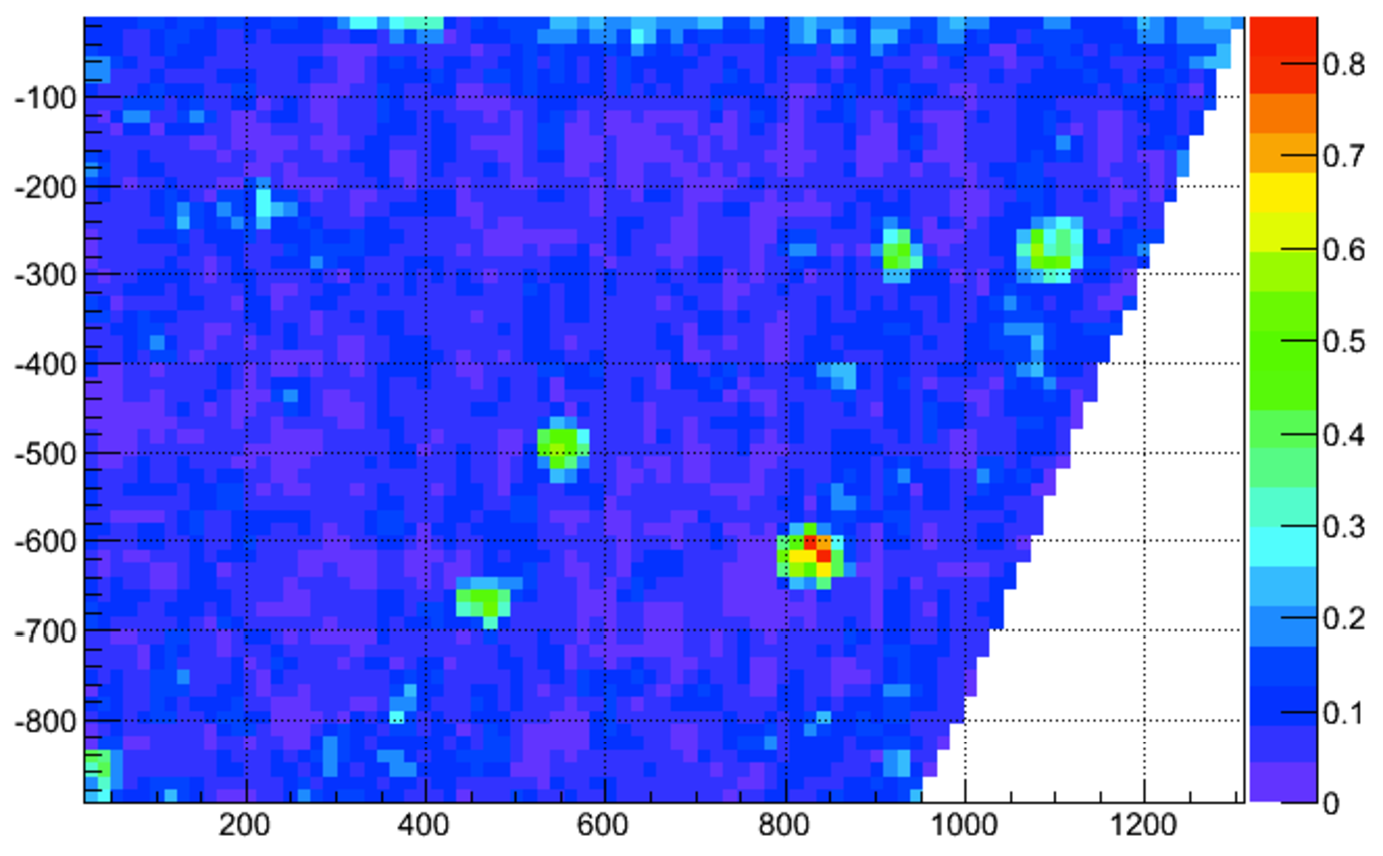
\includegraphics[width=0.45\textwidth]{SlopeML.pdf}
\caption{Profile of the local slope (indicated by the color scale in mrad) of the surface of one of the lateral planar
  mirror measured with a CMM.}
\label{Fig:SlopeML}
\end{center}
\end{figure}

The characterization of the planar mirrors was completed by measuring the reflectivity in a few random spots of
the surface in the wavelength range from 300 to 650~nm. The measurements showed a maximum reflectivity of
approximately 95\% at 400~nm and a reflectivity higher than 90\% in the whole range.

%-----------------------------------------------
\subsection{The Aerogel Radiator}
%-----------------------------------------------

The aerogel radiator was produced by the {\it Budker and Boreskov Institute of Nuclear Physics} (Russia), which was
able to fabricate tiles of different shapes and thicknesses, a critical requirement of the complex CLAS12 geometry.
A total of 102 tiles with nominal refractive index 1.05, cut into squares $200 \times 200$~mm$^2$, as well as
pentagonal, trapezoidal, and triangular shapes, were assembled in two sections. The first section, covering the region
between the beam pipe and the polar angle of 17.5$^\circ$, was made of one layer of 2-cm-thick tiles. The second
section, covering the polar angles between 17.5$^\circ$ and 26$^\circ$, was made of two layers of 3-cm-thick tiles, the
thickest aerogel tiles ever used in Cherenkov radiation applications at this high value of refractive index.

Each tile was tested to determine the geometric and optical parameters~\cite{REF:RICH2016mc}. The measured
geometric parameters are the side length and thickness, and the planarity of the tile surface. The measured optical
parameters include the refractive index at the reference wavelength of 400~nm, and the light transmission as a
function of the wavelength. The transparency parameter $A_0$, the clarity parameter $C$, and the scattering length
$L_{scatt}$ at 400~nm are then extracted from the measured optical parameters using the Hunt parameterization
\cite{REF:Hunt}. Distributions of the measured values of the refractive index, $A_0$ (in percent), and $L_{scatt}$ for the
square 2~cm tiles are shown in Fig.~\ref{Fig:Aerogel_2cm}. The average values obtained over all of the tiles are
$L_{scatt} = 50.5$~mm, $A_0 = 0.975$, and $C = 0.00512$~$\mu$m$^4$/cm. From these measurements, the expected
photon yield for $\beta=1$ particles is estimated to be about 19 photoelectrons (p.e.) in the 2~cm sector and about 25
in the 6~cm (3~cm + 3~cm) sector.

\begin{figure}
\begin{center}
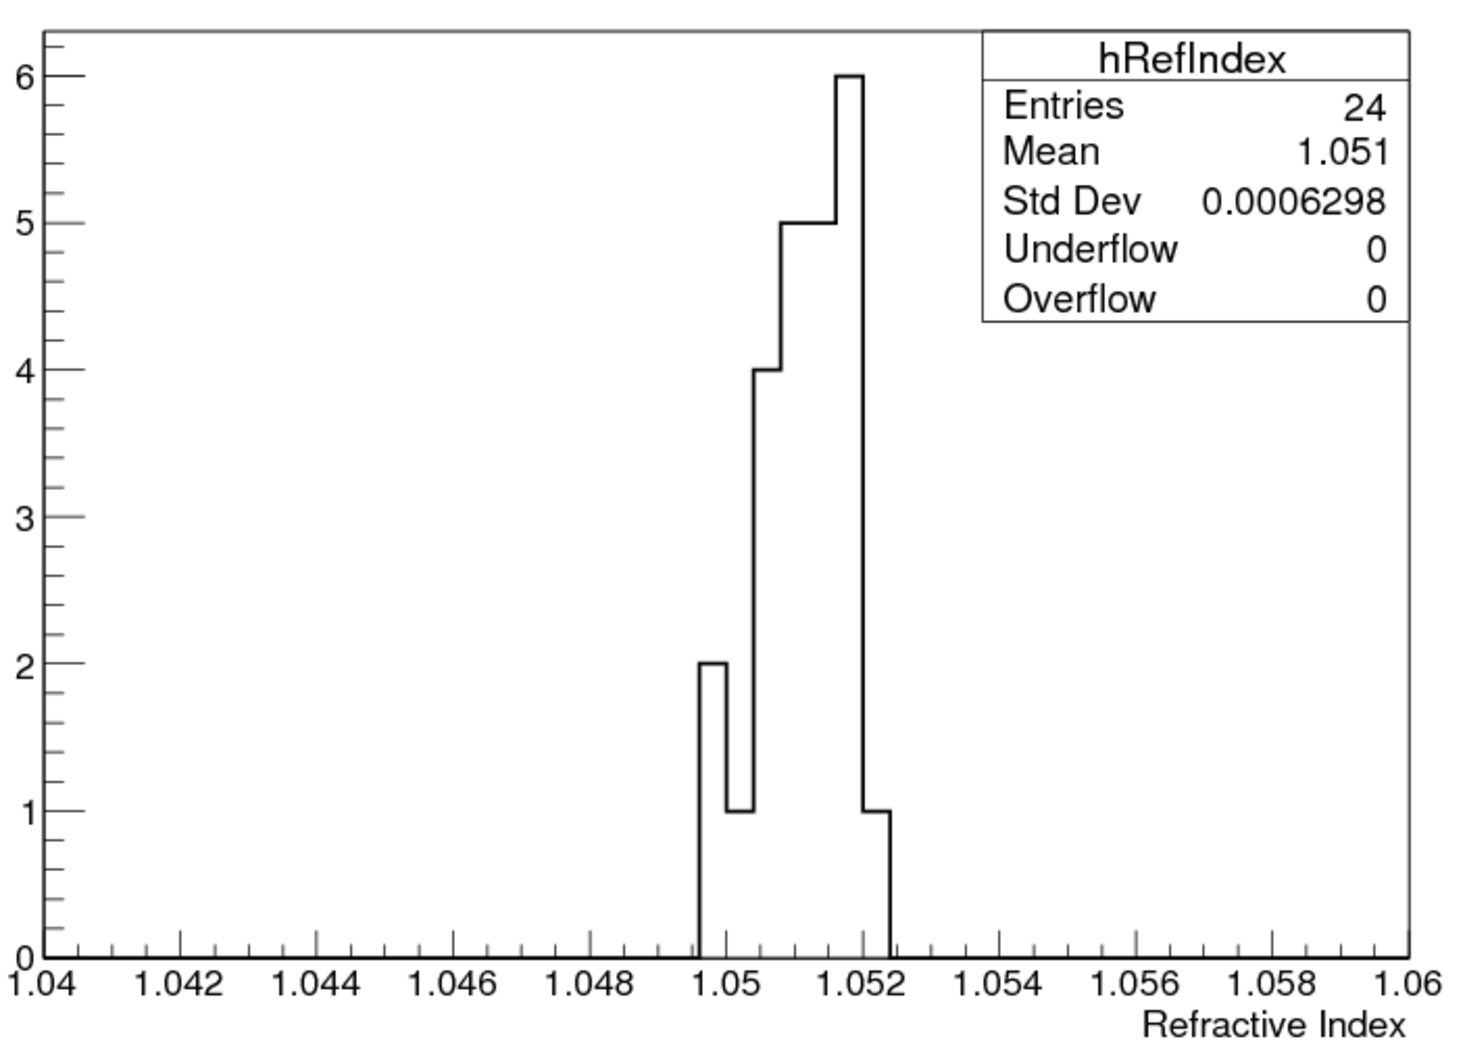
\includegraphics[width=0.35\textwidth]{AeroRefInd_2cm.pdf}
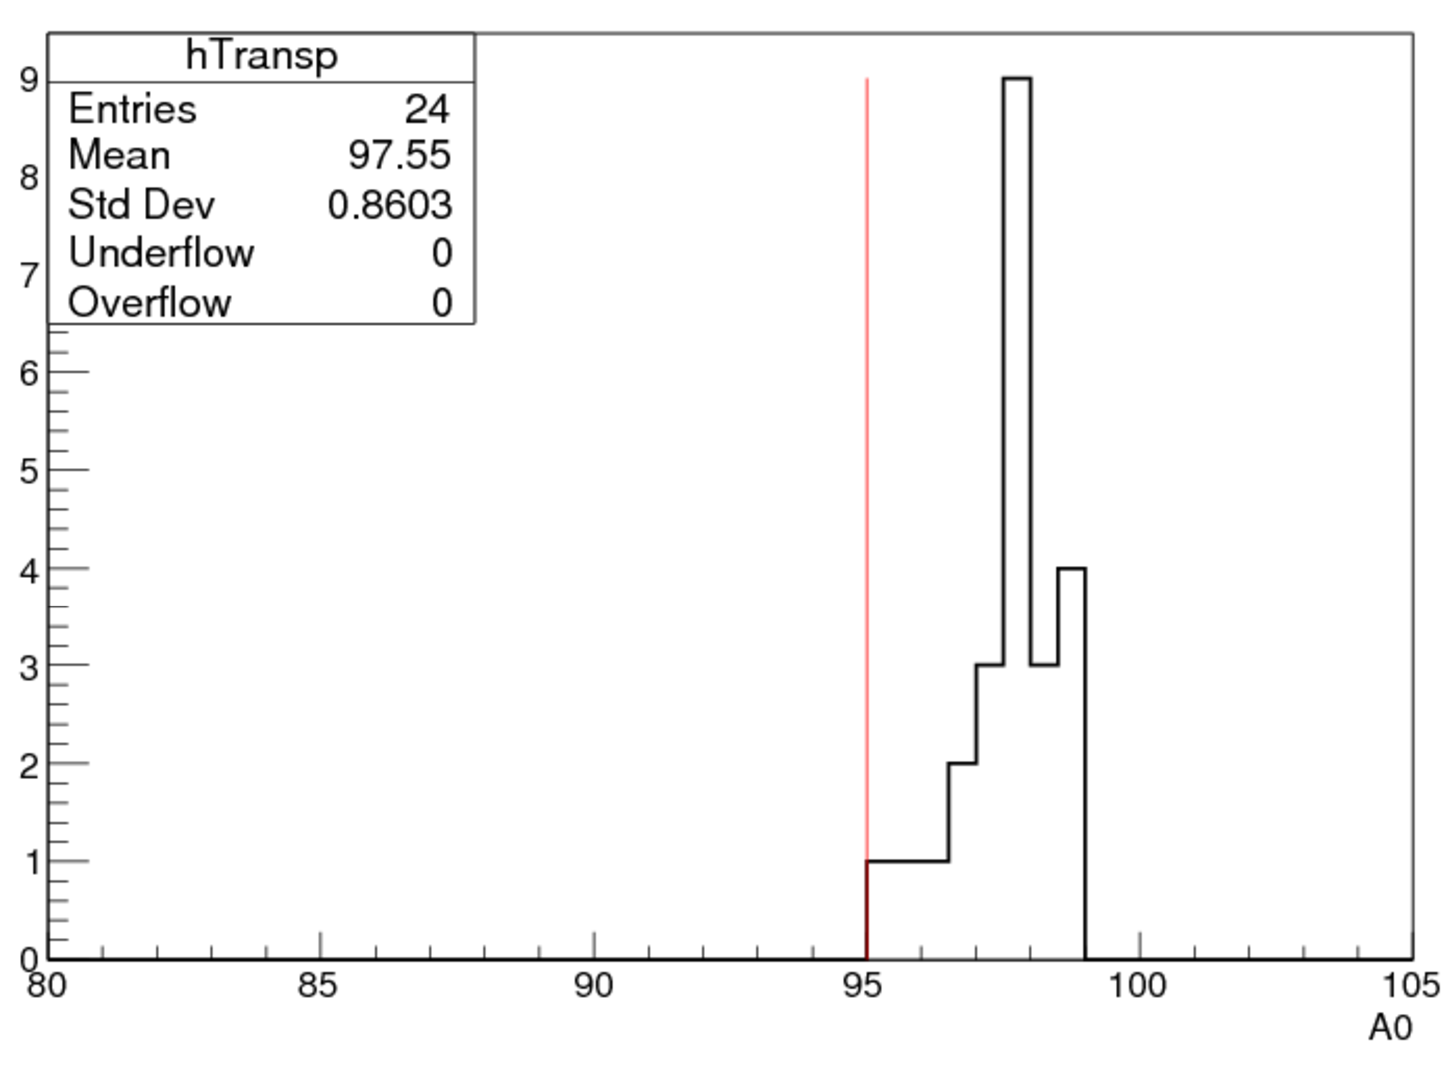
\includegraphics[width=0.35\textwidth]{AeroA0_2cm.pdf}
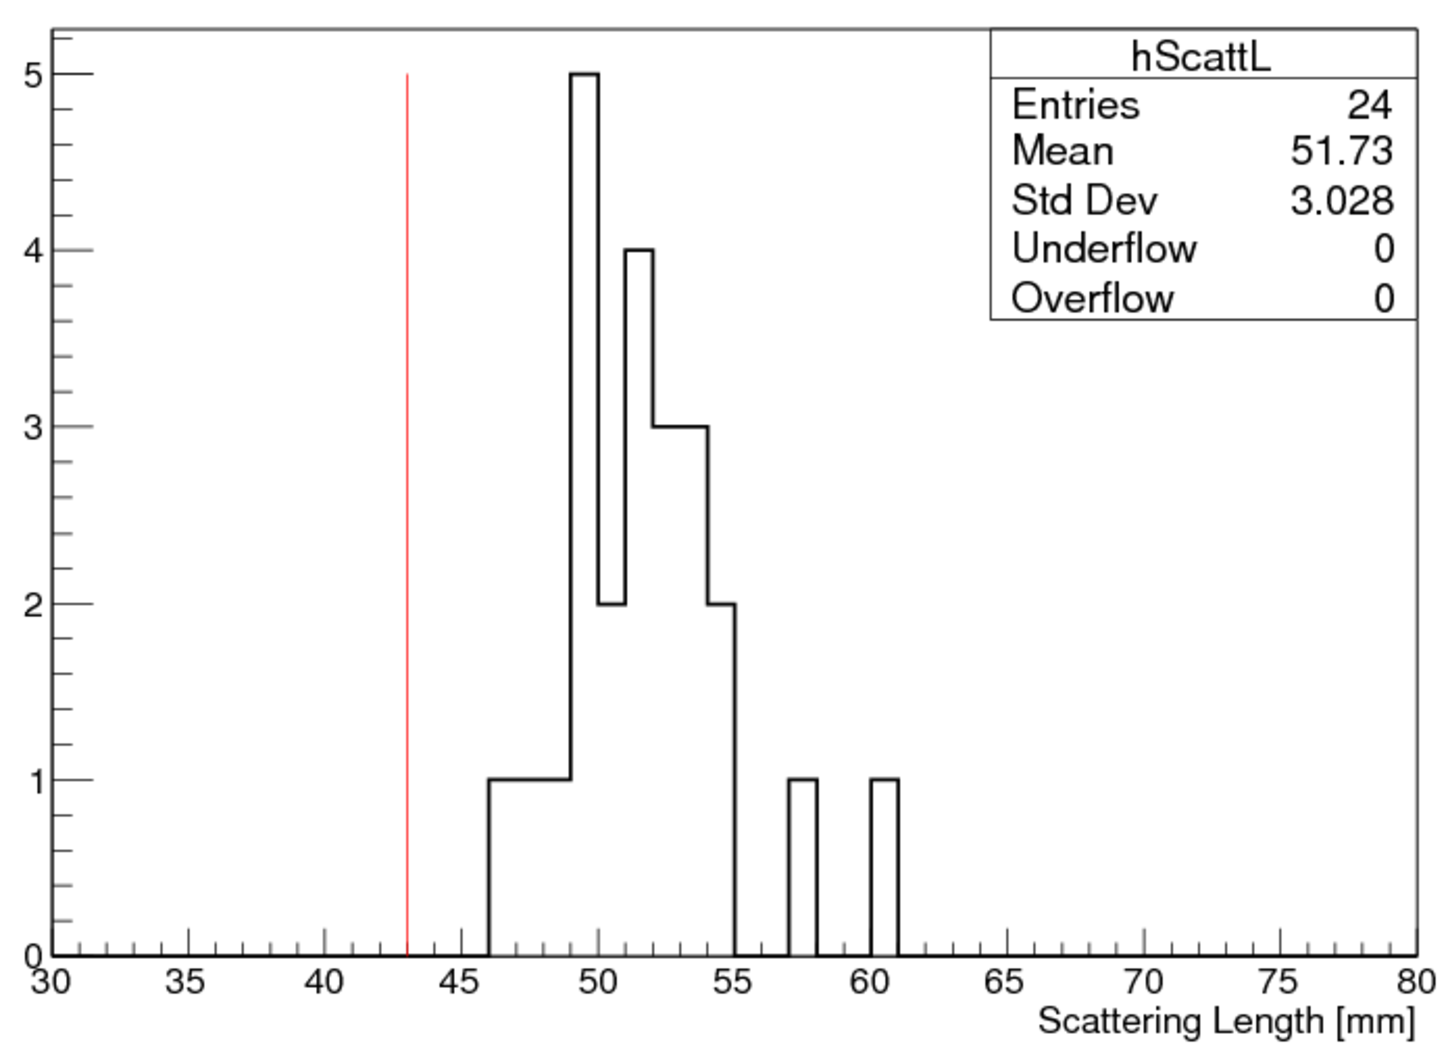
\includegraphics[width=0.35\textwidth]{AeroLscatt_2cm.pdf}
\caption{Distributions of the measured refractive index (top plot), $A_0$ (in percent, central plot), and $L_{scatt}$
  (bottom plot) for the square 2~cm tiles. The red lines indicate the specification limits.}
\label{Fig:Aerogel_2cm}
\end{center}
\end{figure}

%-----------------------------------------------
\subsection{The Photon Detector}
%-----------------------------------------------

Due to the imaging aspects of the RICH, there are several requirements that the photon detector has to fulfill: it has
to efficiently detect single photoelectron (SPE) level signals, it must be sensitive in the visible light wavelengths (due
to the aerogel radiator material), it must have the spatial resolution required to achieve the design angular resolution,
and it has to provide an active area with minimal dead space. In addition, it has to be insensitive to the low torus fringe
field where the RICH readout is located, which is estimated to be 3.5~G maximum, see Fig.~\ref{fig:MagFringe}.
The Hamamatsu flat-panel H8500 Multi-Anode PhotoMultiplier Tube (MaPMT)~\cite{Ref:H8500} with an 8$\times$8
array of $6 \times 6$~mm$^2$ pixels over a compact active area of 5$\times$5~cm$^2$ and with high packing
fractions (89\%), was initially selected as a good candidate.
%Since at the RICH detector position, the CLAS12 torus fringe field is low enough (see Fig.~\ref{fig:MagFringe} ) this allowed us a flexible choice of the photosensor. The Hamamatsu flat-panel H8500 Multi-Anode PhotoMultiplier Tube (\MaPMT)~\cite{Ref:H8500} with an 8x8 array of 5.80 mmx 5.80 mm pixels over a compact active area of 5x5 $\rm cm^2$ area and with high packing fractions (89\%), was selected as a good candidate.
%The goal of the CLAS12 RICH is to achieve a single photon-electron (SPE) Cherenkov angle resolution of 4.5 mrad.
%At the RICH detector position, the CLAS12 torus fringe field is low enough (see Fig.~\ref{fig:MagFringe}) to allow a flexible choice of the photosensor technology.
%Early simulations~\cite{clas12:rich} led to a photosensor spatial resolution below 1~cm to fulfill the design value of 2~mrad angular resolution
%in the direct light configuration.
%The flat panel Hamamatsu H8500 Multi-Anode PhotoMultiplier Tube (\MaPMT)~\cite{Ref:H8500} was selected to achieve the design angular resolution, thanks to the enhanced sensitivity tothe visible and near-UV light in conjunction with a matching geometrical layout of 64 pixels covering a 5x5 $\rm cm^2$ area with an excellent packing factor of 89\%.
Despite not advertised as the optimal choice in the SPE regime, such MaPMTs showed adequate performance in several
laboratory tests~\cite{REF:MaPMT_test} and beam tests~\cite{REF:RICH_CERN}.
%when used in conjunction with an adapted readout electronics.
Just after the RICH construction startup, the novel Hamamatsu H12700 became available, with the same layout as
the H8500, but an optimized dynode structure for single photon detection~\cite{Ref:H12700}.

Of the 391 MaPMTs that the CLAS12 RICH employs, 80 are of the H8500 type and the rest are of the H12700 type.
This results in a total of 25024 individual pixels, covering the $\sim$1~m$^2$ trapezoidal active area of the first
RICH module.
% and it is the first large-area detector to employ this new multi-anode photo-multipliers. 
The production specifications included requirements on the minimum gain of $1 \times 10^6$ and a maximum total dark
current of 5~nA. Both were fully achieved. Figure~\ref{fig:MaPMTGain} shows the distribution of the pixel gains, with
has an average value of $2.7 \times 10^6$, corresponding to about 400~fC generated charge per SPE.

\begin{figure}[t]
\begin{center}
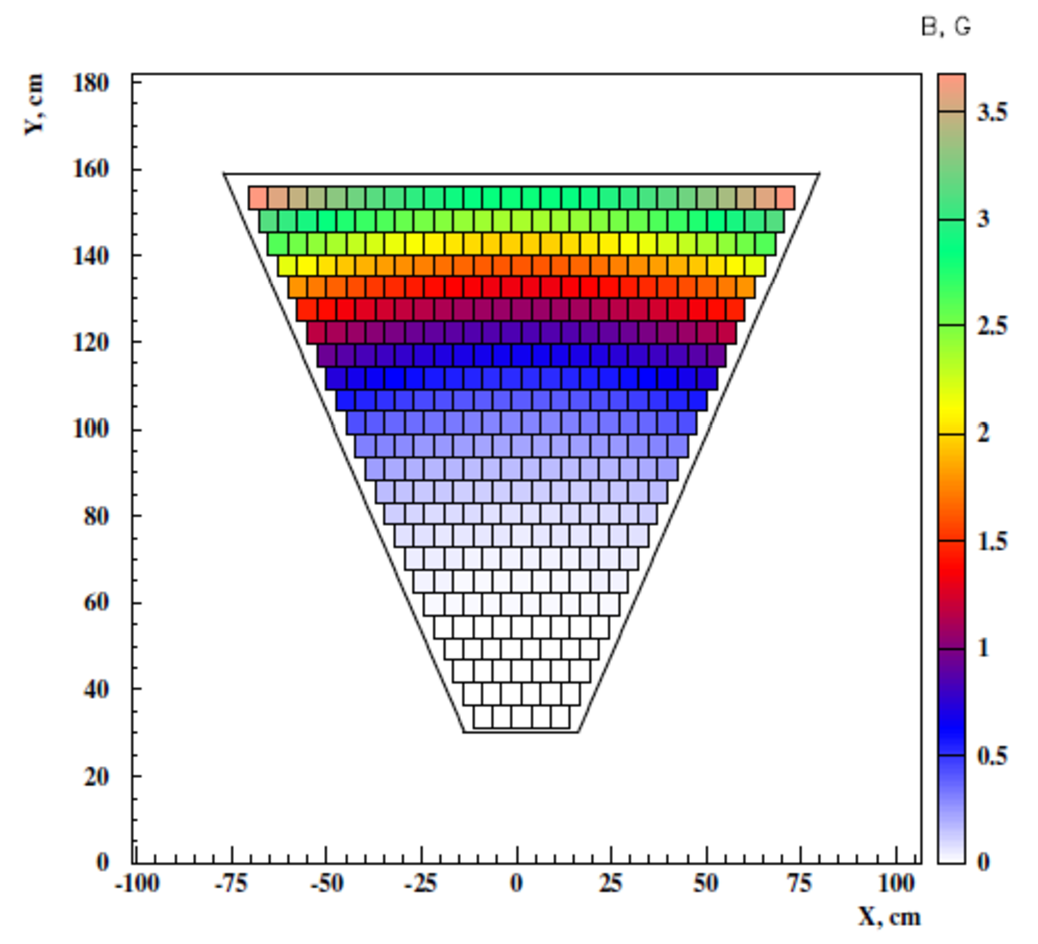
\includegraphics[width=0.85\columnwidth]{Field.pdf}
\end{center}
\caption{Calculated map of the torus fringe field strength (in Gauss) in the RICH photodetector area.}
\label{fig:MagFringe}
\end{figure}

\begin{figure}[t]
\begin{center}
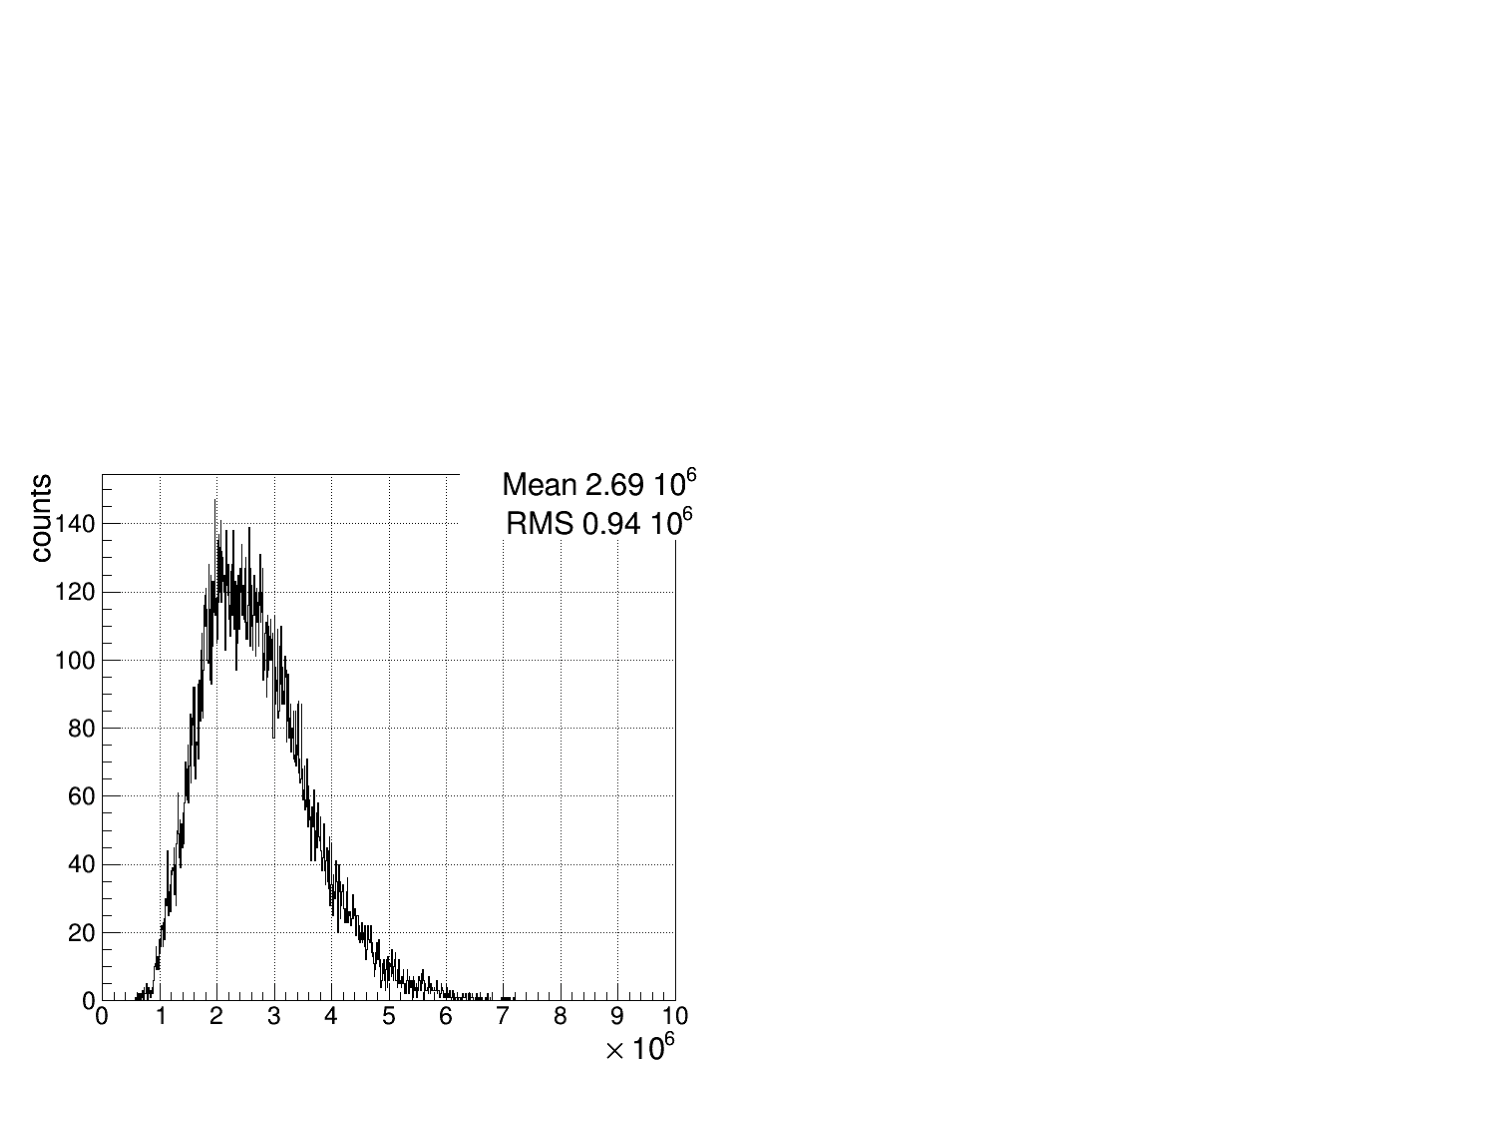
\includegraphics[width=0.85\columnwidth]{Gain.pdf}
\end{center}
\caption{Distribution of the data-sheet gains of the 25000 RICH MaPMT channels.}
\label{fig:MaPMTGain}
\end{figure}

%-----------------------------------------------
\subsection{The Readout Electronics}
%-----------------------------------------------

\begin{figure}[t]
\begin{center}
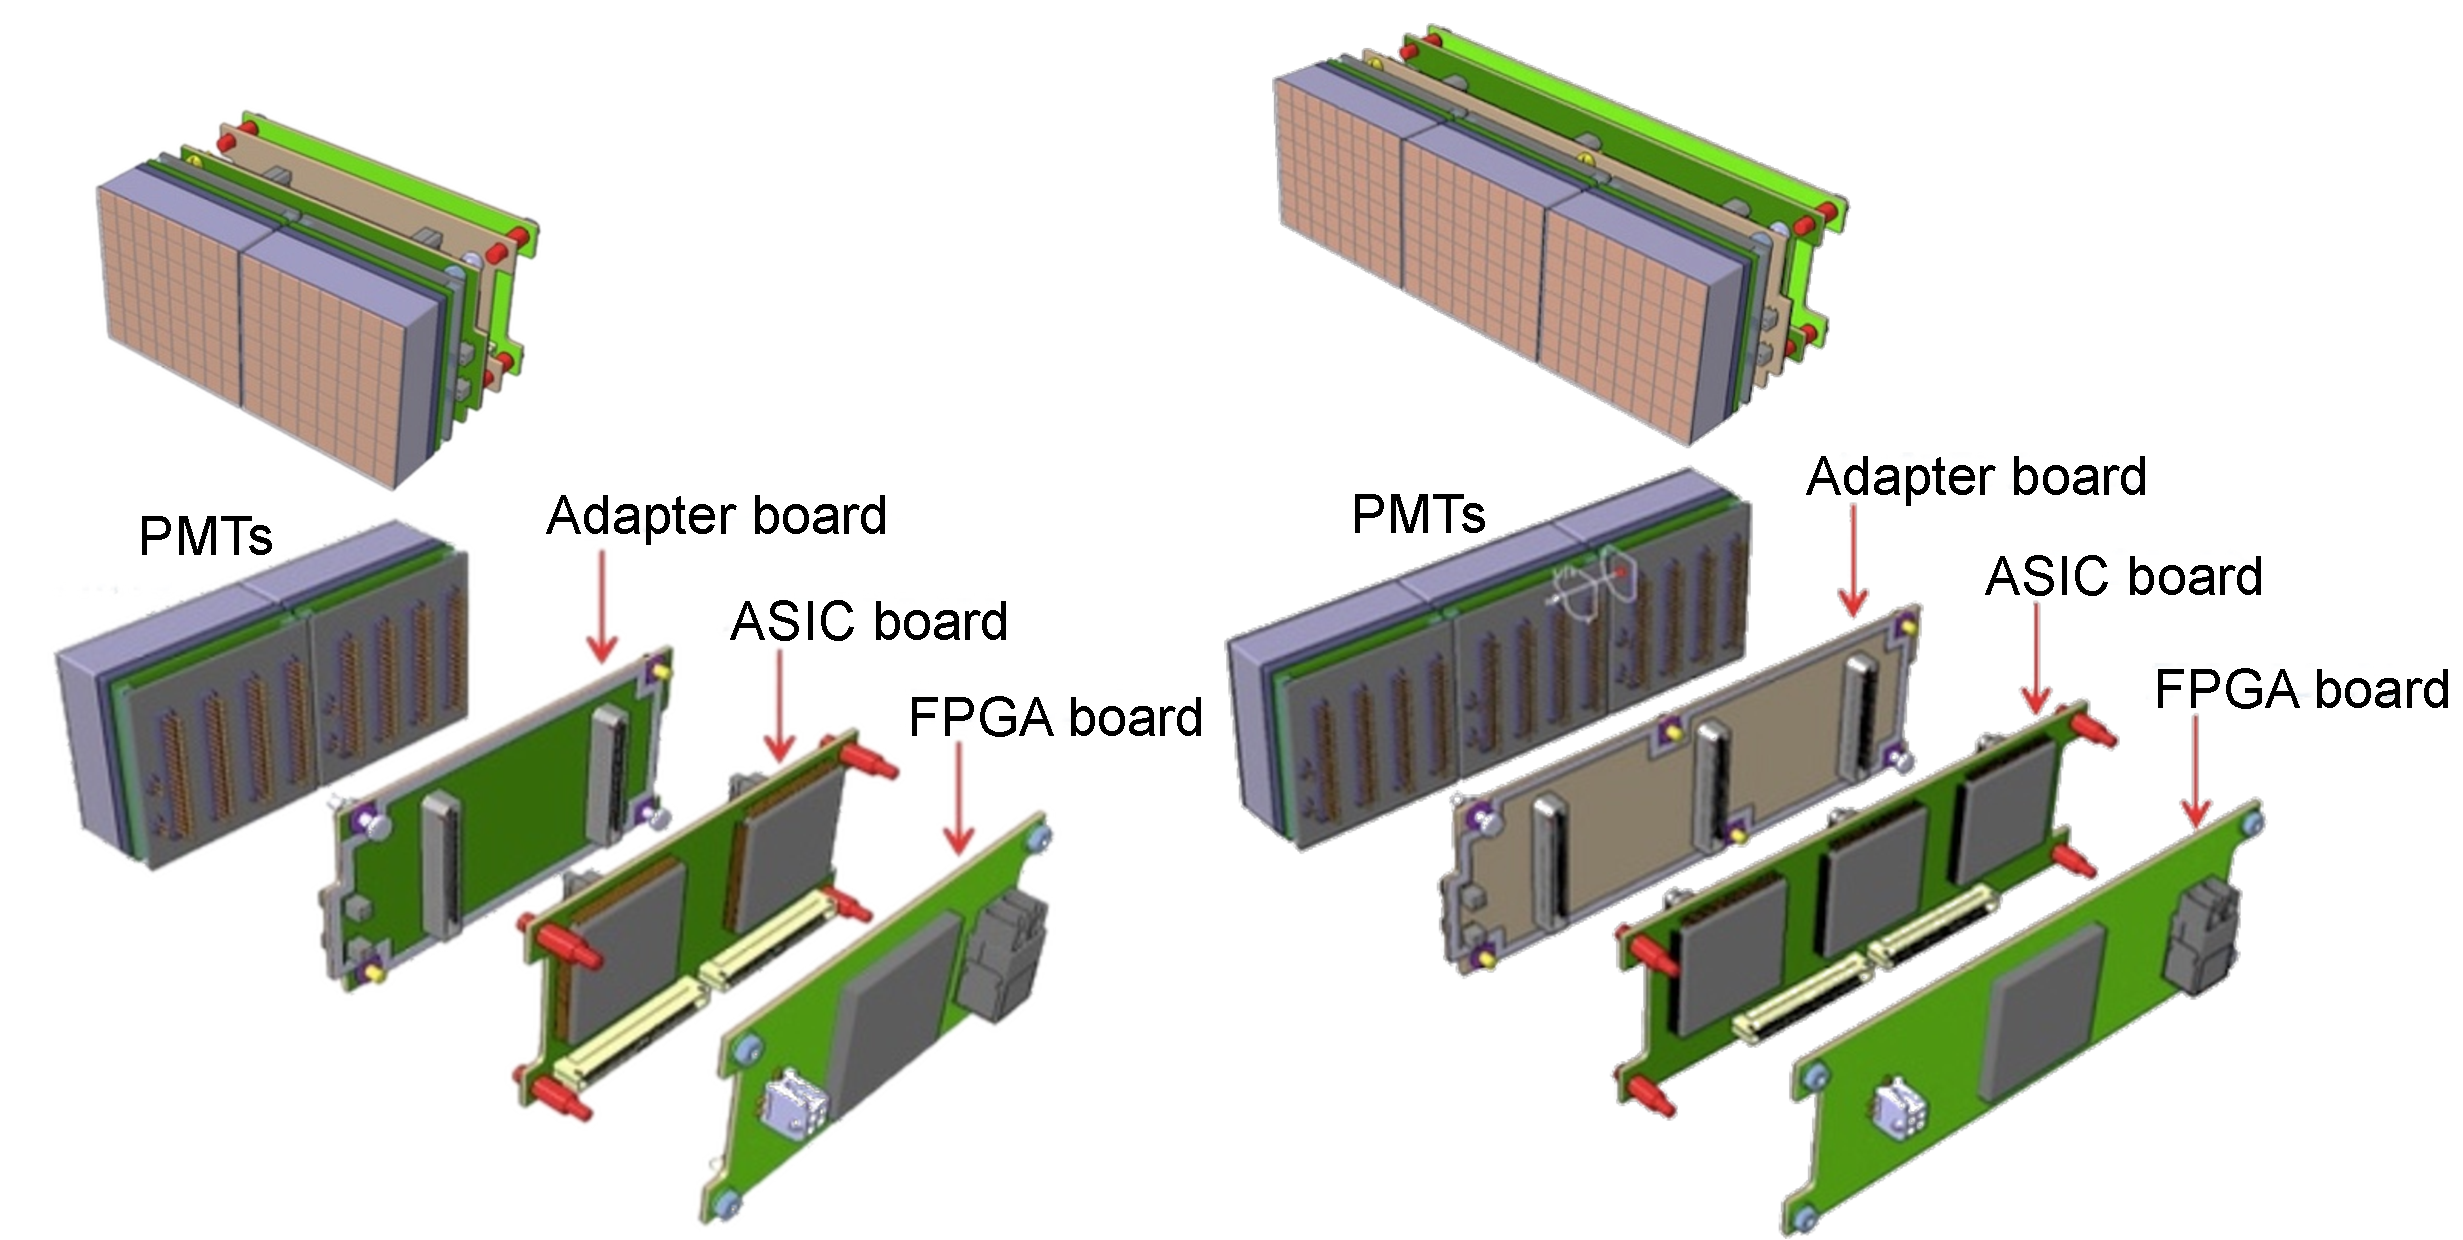
\includegraphics[width=1.00\columnwidth]{TileAssembly.pdf}
\end{center}
\caption{The CLAS12 RICH readout unit design (see text for details).}
\label{fig:EleTile}
\end{figure}

The RICH front-end electronics are designed to ensure 100\% efficiency at 1/3 of the average photoelectron signal
level, 1 to 4 gain spread compensation, time resolution of the order of 1~ns to distinguish direct from reflected photon
hits, and a trigger rate up to 20~kHz with 8~$\mu$s trigger latency.

The front-end electronics are organized into compact units (called tiles, see Fig.~\ref{fig:EleTile}) mechanically designed to
fit the MaPMT dimensions, each serving two or three MaPMTs, thus allowing the tessellation of large surfaces with
minimum dead space and material budget. Each readout unit comprises three boards with complementary functions.

A feed-through adapter board provides the electrical connectivity of the sensors with the external readout
system, while preserving the adequate light and gas tightness of the inner detector volume when mounted on the RICH
carbon fiber supporting panel. It also distributes the sensor bias voltage (with -1000~V as nominal value).

The signal processing board is based on the MAROC3 chip~\cite{MAROC3:chip}, a 64-channel microcircuit
dedicated to MaPMT pulse processing. Each channel comprises a low impedance adjustable gain preamplifier followed
by two highly configurable shaping sections with independent processing. The first section embeds a slow shaper and
a sample and hold structure to allow linear charge measurements up to 5~pC. Requiring short trigger delays and
multiplexed access, this section can be used as a RICH calibration tool. The second section features a fast shaper and
an adjustable threshold discriminator to produce, for each input signal, a start and stop logic pulse. A constant-threshold
binary readout requires good stability of the baseline (pedestal) and definition of the working point (gain and
threshold). During the board production, quality assurance tests confirmed the excellent sensitivity of the logical
readout, able to discriminate signals down to a few percent of a single photoelectron discharge, as will be extensively
discussed in Section~\ref{sec:Commissioning}.

The third stage of the readout is made of the FPGA boards, hosting a Xilinx7 FPGA chip, responsible for configuring
and reading the front-end MAROC3, distributing the trigger, and interfacing with the data acquisition system
\cite{daq-nim} via optical link. The FPGA provides a TDC functionality with a 1 ns time stamp for both start and stop
times. The start time is used for timing purposes, while the difference between the stop and start times, the so-called
Time-Over-Threshold (ToT), provides a non-linear estimate of the amplitude of the input signal and is used for the
time-walk correction, see Section~\ref{sec:TimeCalib}. Finally, the FPGAs also embed a self-trigger scaler readout that is used
as a calibration and monitor tool.

%-----------------------------------------------
\subsubsection{MaPMT Characterization}
%-----------------------------------------------
\label{sec:FEtests}

The characterization of hundreds of MaPMTs is a  challenging problem. In order to test them efficiently within a
reasonable time frame, a fully automated test stand was built to evaluate 6 MaPMTs at once. The test stand consists
of a 470~nm diode laser system, 2 long travel motorized stands to drive a laser fiber in two-dimensional space for
individual pixel illumination, and a motorized neutral density filter system. The laser light is directed through the
fiber and attenuated to the single photon level using neutral density filters to mimic the conditions of the RICH
detector. The motors are remotely controlled to move the focused laser 1 mm beam spot across the entire surface of the MaPMT
entrance window and illuminate one by one the 64 pixels individually (see Fig.~\ref{fig:beamopt1}). Alternatively, one
can illuminate the whole surface of the MaPMT photocathode at once using an Engineered Diffuser to produce a square
pattern with a non-Gaussian intensity distribution (see Fig.~\ref{fig:beamopt2}). The latter configuration was used for the
massive characterization of the RICH MaPMTs, bringing routine workloads to a minimum. The evaluation of 6 MaPMTs
(corresponding to 384 individual channels) at 4 different high voltages and 6 different light intensities was completed
in 6 hours with less than 15 minutes of human intervention.

\begin{figure}[bt]
	\centering
	\begin{subfigure}[b]{0.628\linewidth}
		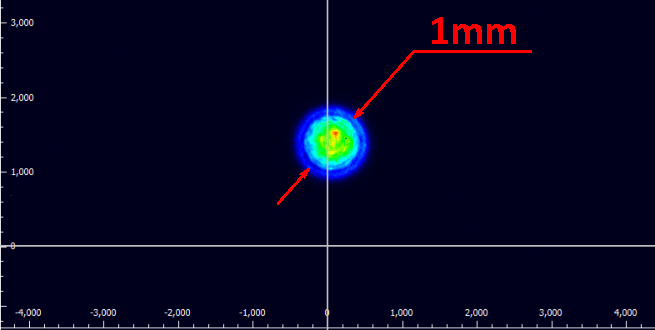
\includegraphics[width=\textwidth]{beamspot.pdf}
		\caption{Focused laser beam.}
		\label{fig:beamopt1}
	\end{subfigure}
	\begin{subfigure}[b]{0.354\linewidth}
		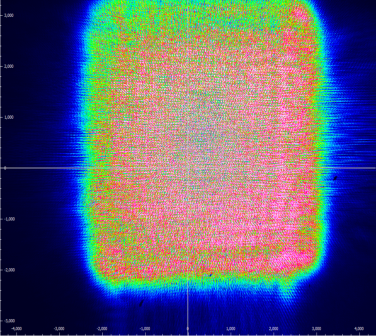
\includegraphics[width=\textwidth]{beamsquare.pdf}
		\caption{Square pattern.}
		\label{fig:beamopt2}
	\end{subfigure}
	\caption{The MaPMT test stand laser output options.}
\end{figure}

The characteristics of the SPE spectrum were studied using the charge measurement functionality of the slow shaper
of the MAROC3 chip. A new computational model~\cite{Pavel} for the description of the photomultiplier response
functions of both the H8500 and H12700 MaPMTs was developed. Important features of the model include the ability
to approximate the true SPE spectra from different PMTs with a variety of
parameterized spectral shapes.
%, reflecting the variability in the design and in the individual parameters of the detectors. The new techniques were developed in the process of building the model, such as the method of decomposition of the spectra into a series of elementary Poisson probability density functions, and the use of convolution algebra to build the multi-photoelectron amplitude distributions describing measured spectra. 
The predictive power of the model was tested by demonstrating that the SPE spectral parameters, obtained in the
measurements, may describe well the amplitude distributions of the same photodetector measured at different levels
of illumination. Thus, the model allowed us to extract the characteristic parameters of the devices independently of the test measurement conditions.

The SPE spectrum is extracted by fitting with the model function the signal amplitude distribution measured 
as shown in Fig.~\ref{fig:SPEH8500} for the H8500 MaPMT and in Fig.~\ref{fig:SPEH12700} for the H12700.
The $x$-axis is calibrated in terms of charge measured by the MAROC3 chip.
%The probability of an initial photon to knock out $m$ photoelectrons is distributed according to the Poissonian $P(m;\mu)=\frac{\mu^me^{-\mu}}{m!}$.
%To approximate the performance of the first amplification cascade of the MaPMT the probability function $T(n,m;\bf{t})$ was introduced in the model as trinomial sum of three Poissoanians with different average secondary multiplicities and the corresponding three relative probabilities for every photoelectron to generate secondary electrons, here $m$ is the number of the electrons knocked out from the first dynode and $n$ is the number of electrons emitted out of the second dynode.
To approximate the performance of the first amplification cascade of the MaPMTs, the probability function
$T(n,m;{\bf t})$ was introduced in the model as a trinomial sum of three Poissonians with different average secondary
multiplicities and the corresponding three relative probabilities for every photoelectron to generate secondary
electrons. In the function, $m$ is the number of the electrons knocked out from the first dynode, $n$ is the number
of electrons emitted out of the second dynode, and ${\bf t}$ is the vector of the model parameters
(see Ref.~\cite{Pavel} for more details).

In each fit, the parameter $\mu$ corresponds to the average number of photoelectrons created at the photocathode by
each laser pulse, $\nu_{average}$ is the average number of secondary electrons generated at the first dynode, and $scale$ is the 
average anode charge collected from one photoelectron. 
 
\begin{figure}[bth]
	\centering
	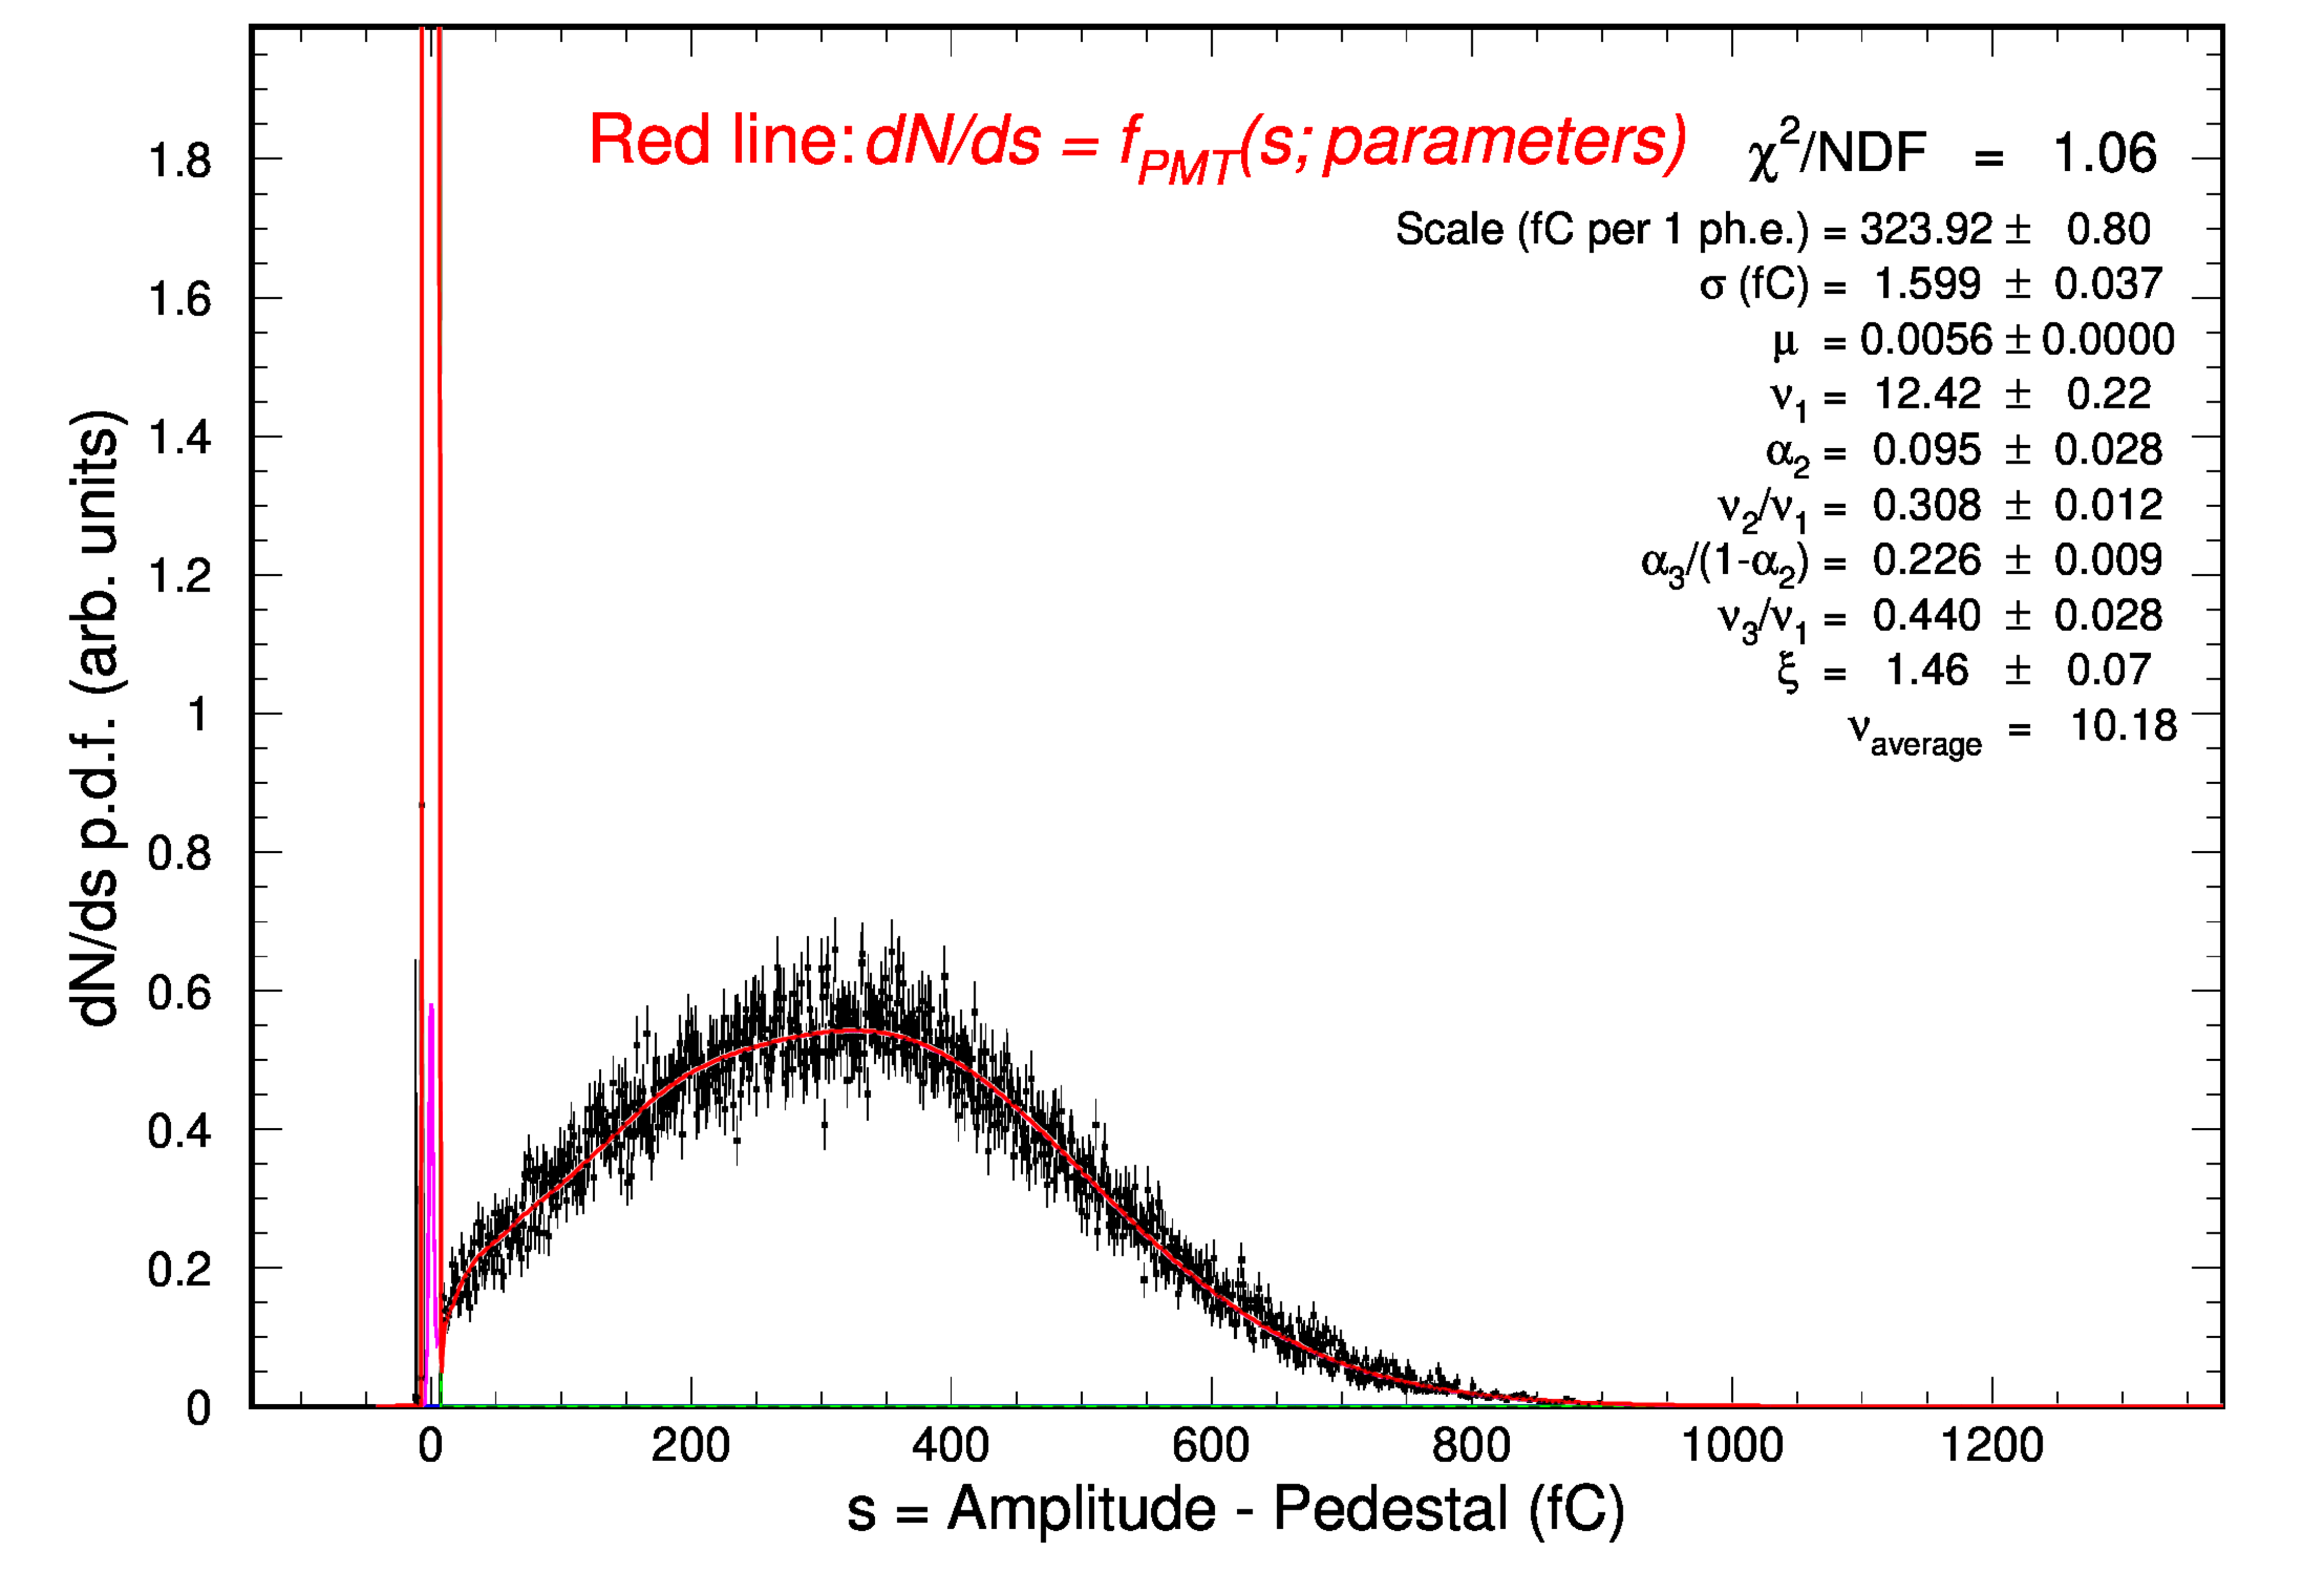
\includegraphics[width=\linewidth]{H8500-r-W0-CA7709-w3-g064-v1000-t227-37.pdf}
	\caption{Sampled H8500 \MaPMT single photoelectron spectrum from one of the pixels at 1000~V with a low-intensity
          laser light source. The fit function (see details in Ref.~\cite{Pavel}) is shown as a solid line. 
          The relevant parameters (see text) are $\mu=0.0056$, $\nu_{average}=10.18$ and $scale=323.9$~fC. This corresponds
          to a PMT gain=$2.0 \times 10^6$.
          %The parameter
          %$\mu=0.0056$ corresponds to the average number of photoelectrons created at the photocathode by 
          %each laser pulse,  $\nu_{average}=10.18$ is  the average number of secondary electrons generated at the first
          %dynode, and $scale=323.9$~fC is the average anode charge collected from one photoelectron. This corresponds
          %to a PMT gain=$2.0 \times 10^6$.} 
          }
	\label{fig:SPEH8500}
\end{figure}

\begin{figure}[ht]
	\centering
	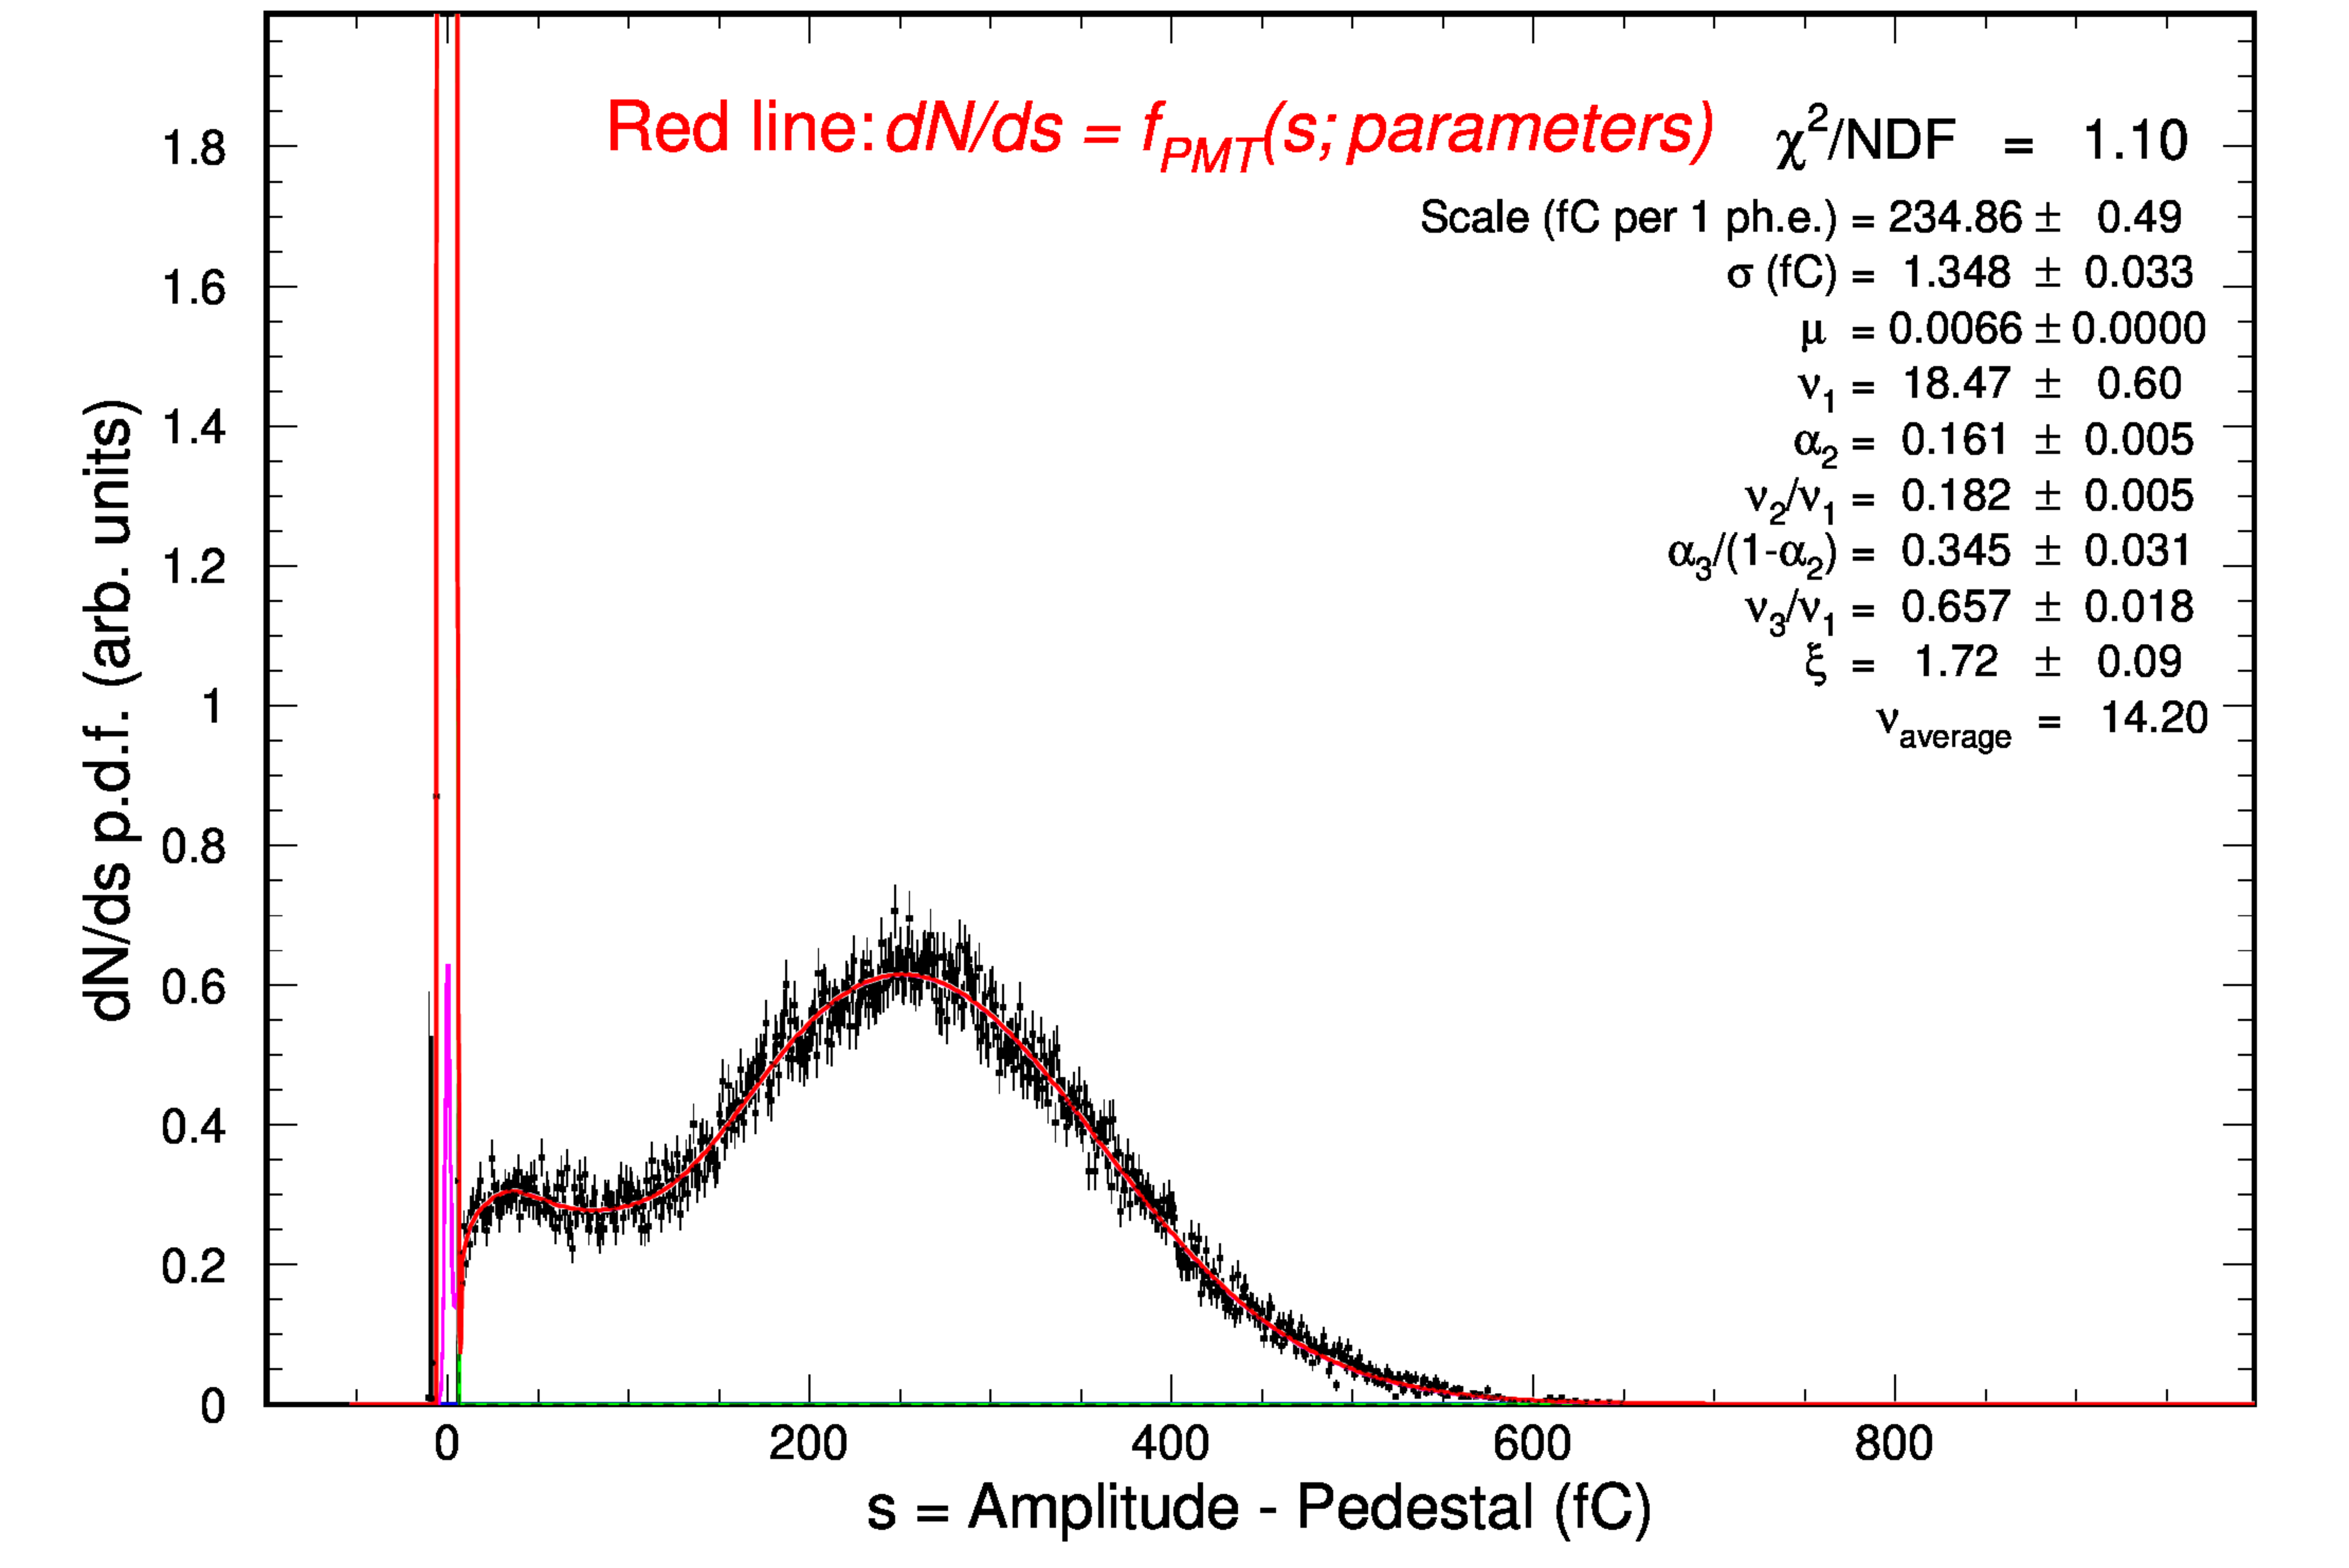
\includegraphics[width=\linewidth]{H12700-r-W0-GA0982-w3-g064-v1000-t227-37.pdf}
	\caption{Sampled H12700 \MaPMT single photoelectron spectrum from one of the pixels at 1000~V with a low-intensity
          laser light source. The fit function (see details in Ref.~\cite{Pavel}) is shown as a solid line. 
          The relevant parameters (see text) are $\mu=0.0066$, $\nu_{average}=14.18$ and $scale=234.8$~fC. This corresponds
          to a PMT gain=$1.5 \times 10^6$.
          %The parameter
          %$\mu=0.0066$ corresponds to the average number of photoelectrons created at the photocathode by
          %each laser pulse, $\nu_{average}=14.2$ is the average number of secondary electrons generated at the first
          %dynode, and $scale=234.8$~fC is the average anode charge collected from one photoelectron. This corresponds
          %to a PMT gain=$1.5 \times 10^6$.}
          }
	\label{fig:SPEH12700}
\end{figure}

The data showed that the H12700 has, on average, a 10\% better efficiency than the H8500, likely due to the improved
photocathode performance and collection efficiency. An example of the results for one MaPMT is shown in
Fig.~\ref{fig:PavelPassport}. 
The parameter $scale$ (top plot), characterizing the amplification (dynode) system, is
virtually independent of the light radiation level, while strongly dependent on the high voltage supply, the exact behavior one would expect from the characteristic  of internal dynode system of a MaPMT. 
The central plot shows the average number of photoelectrons $\mu$ measured with different optical filters. It indicates that all of the channels respond in the same way as the light intensity increases.
This parameter is independent of the light intensity as expected.
The parameter $\nu_{average}$
(bottom plot) that is related to the first dynode performance,  has week dependence on the bias voltage  and independent on the level of light radiation as well. 
\begin{figure}[h]
\begin{center}
%	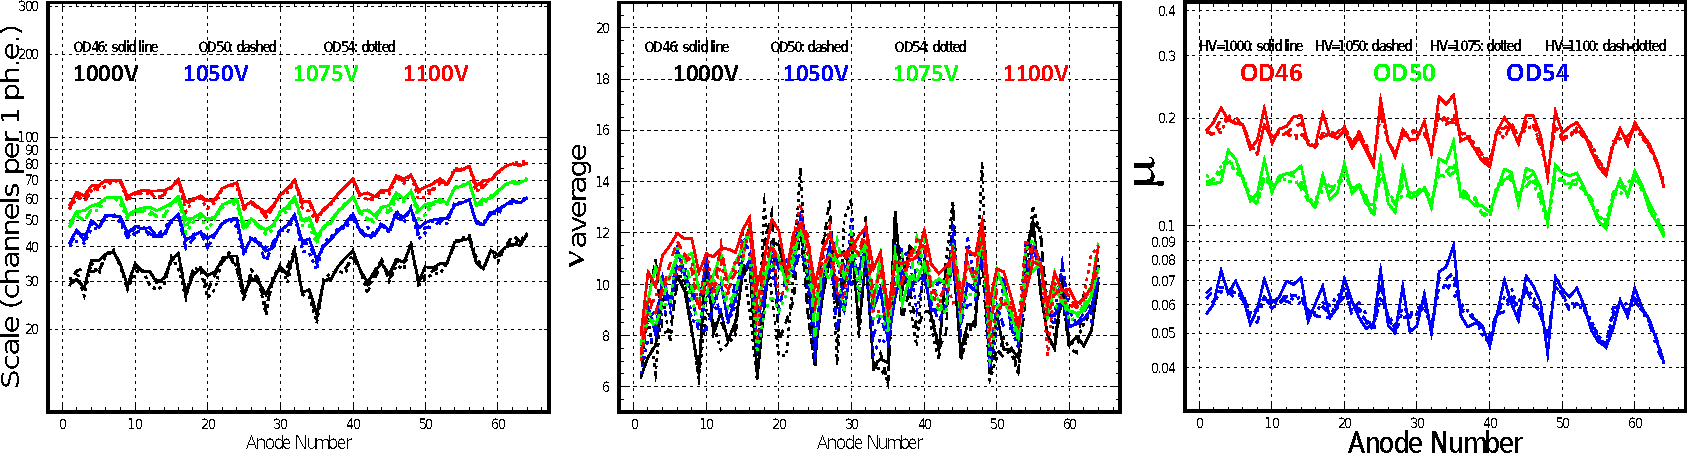
\includegraphics[width=\linewidth]{PavelPassport.pdf}
	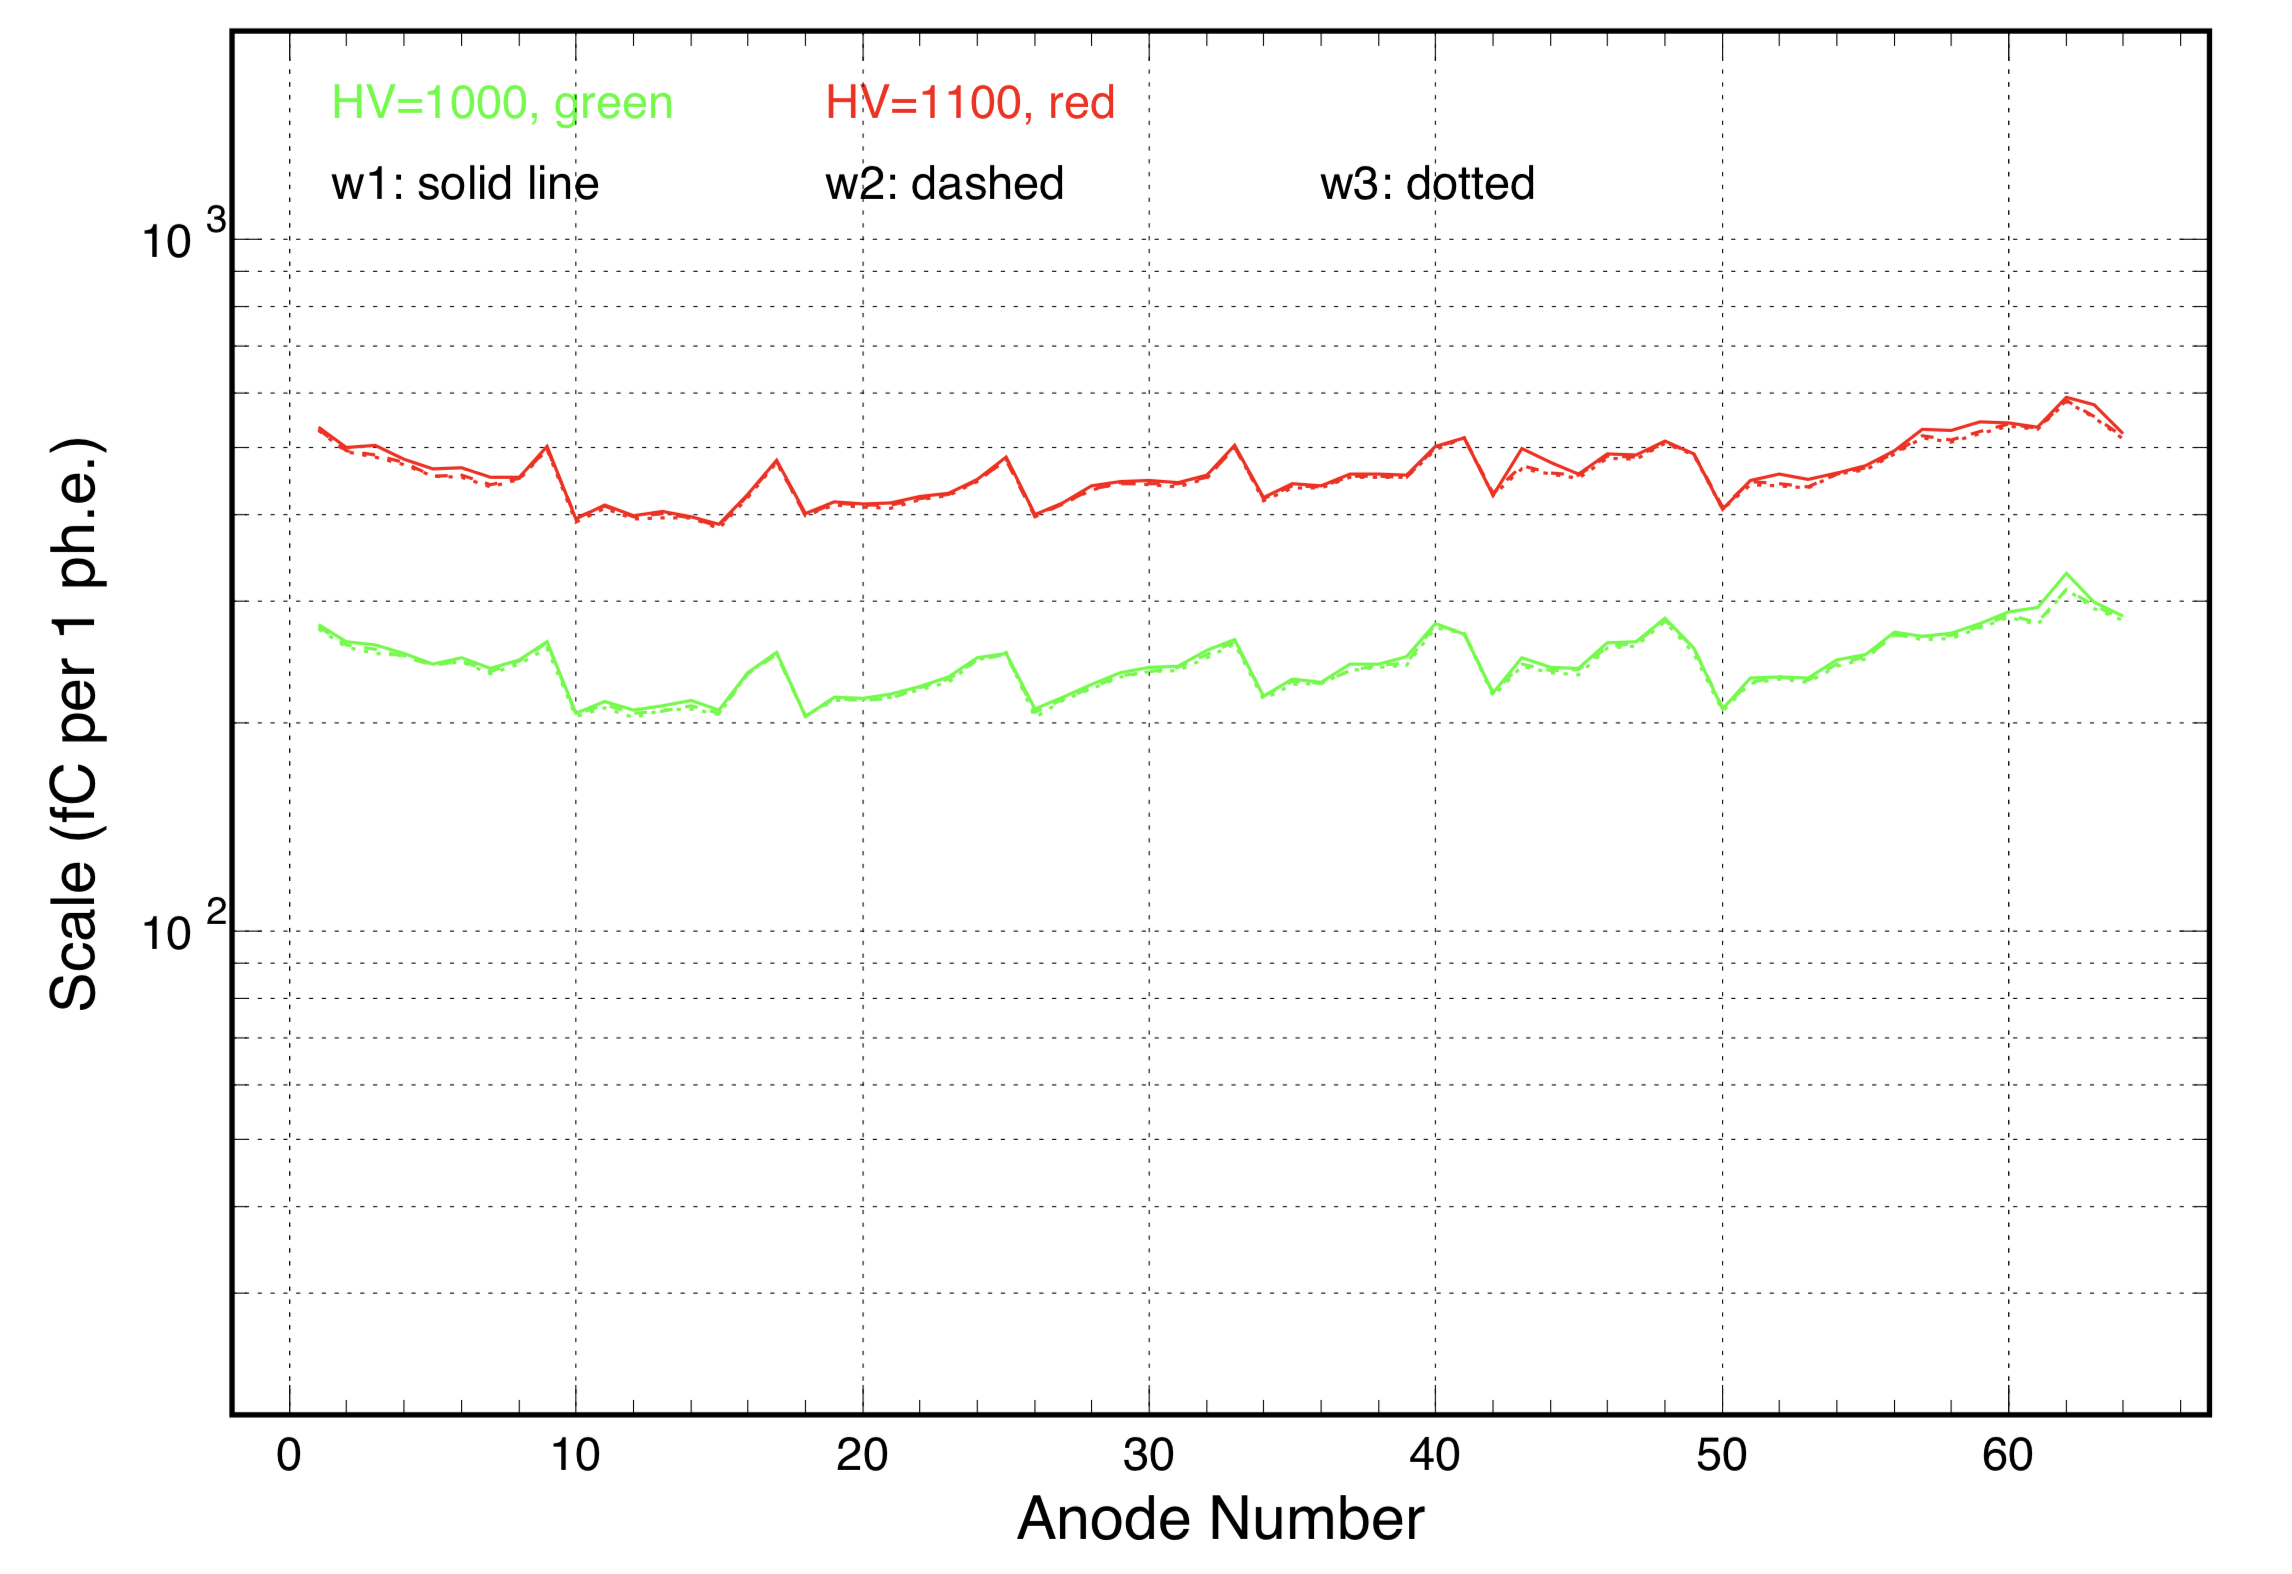
\includegraphics[width=0.95\linewidth]{H12700_scale.png}
	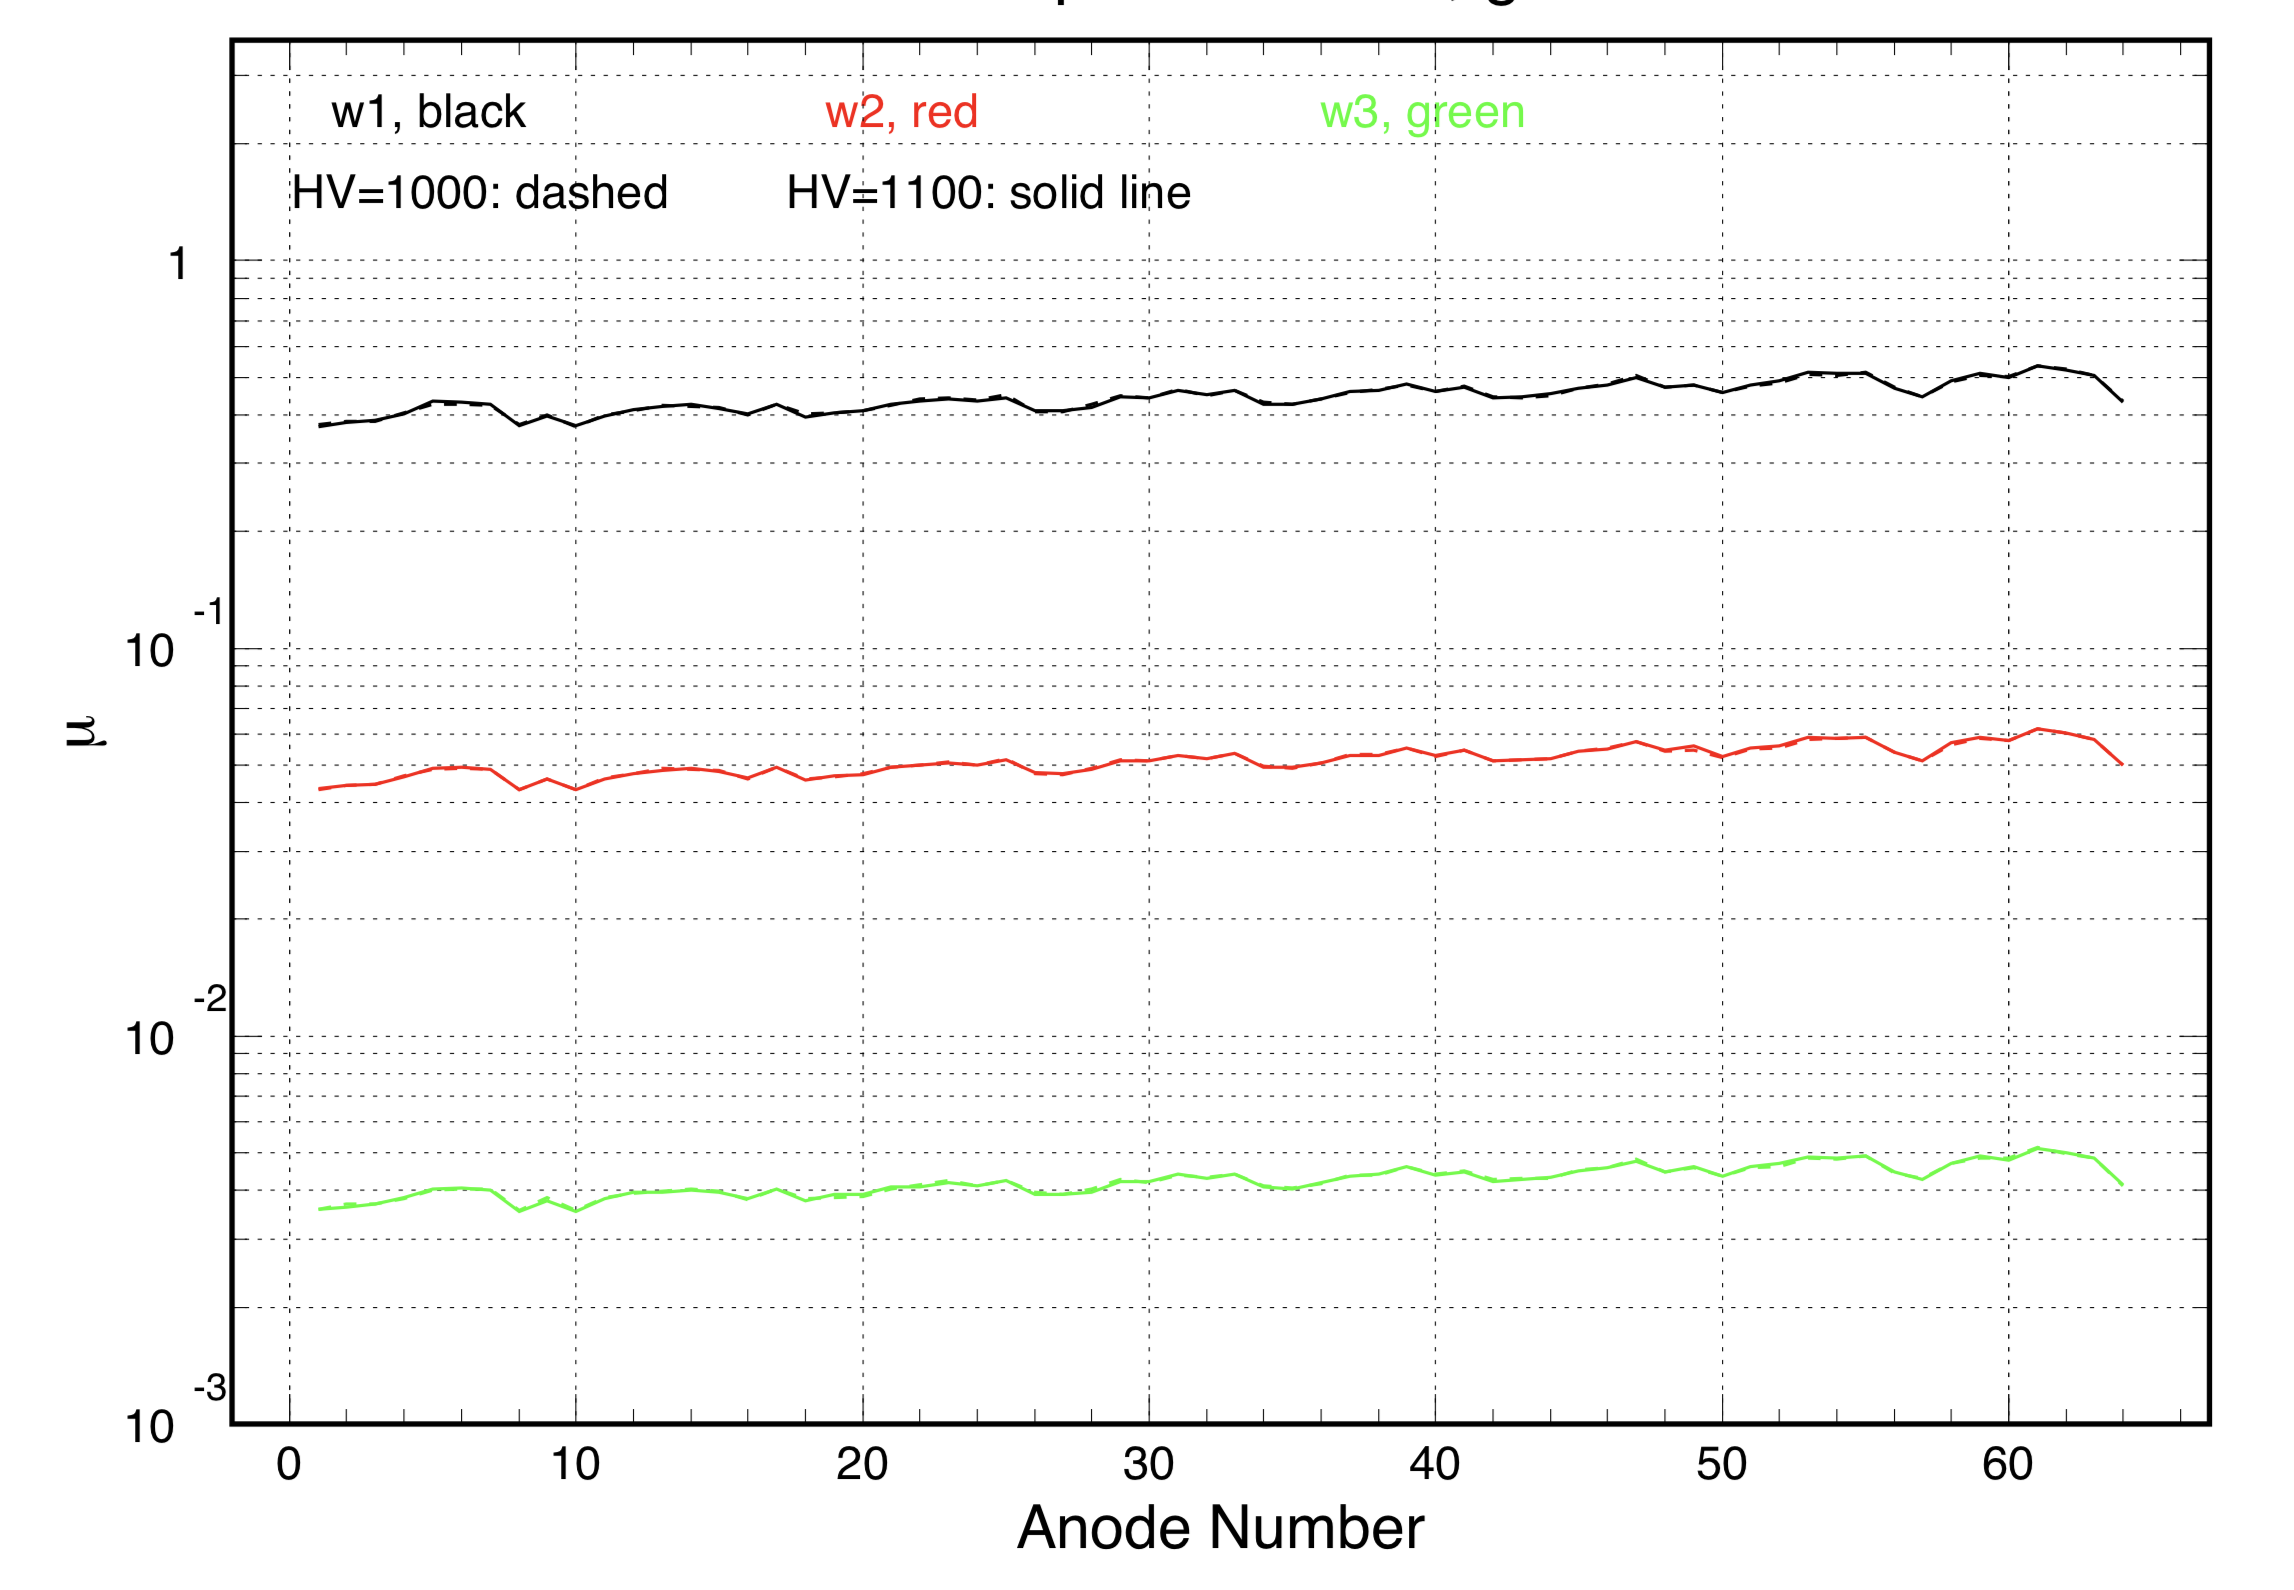
\includegraphics[width=0.95\linewidth]{H12700_mu.png}
	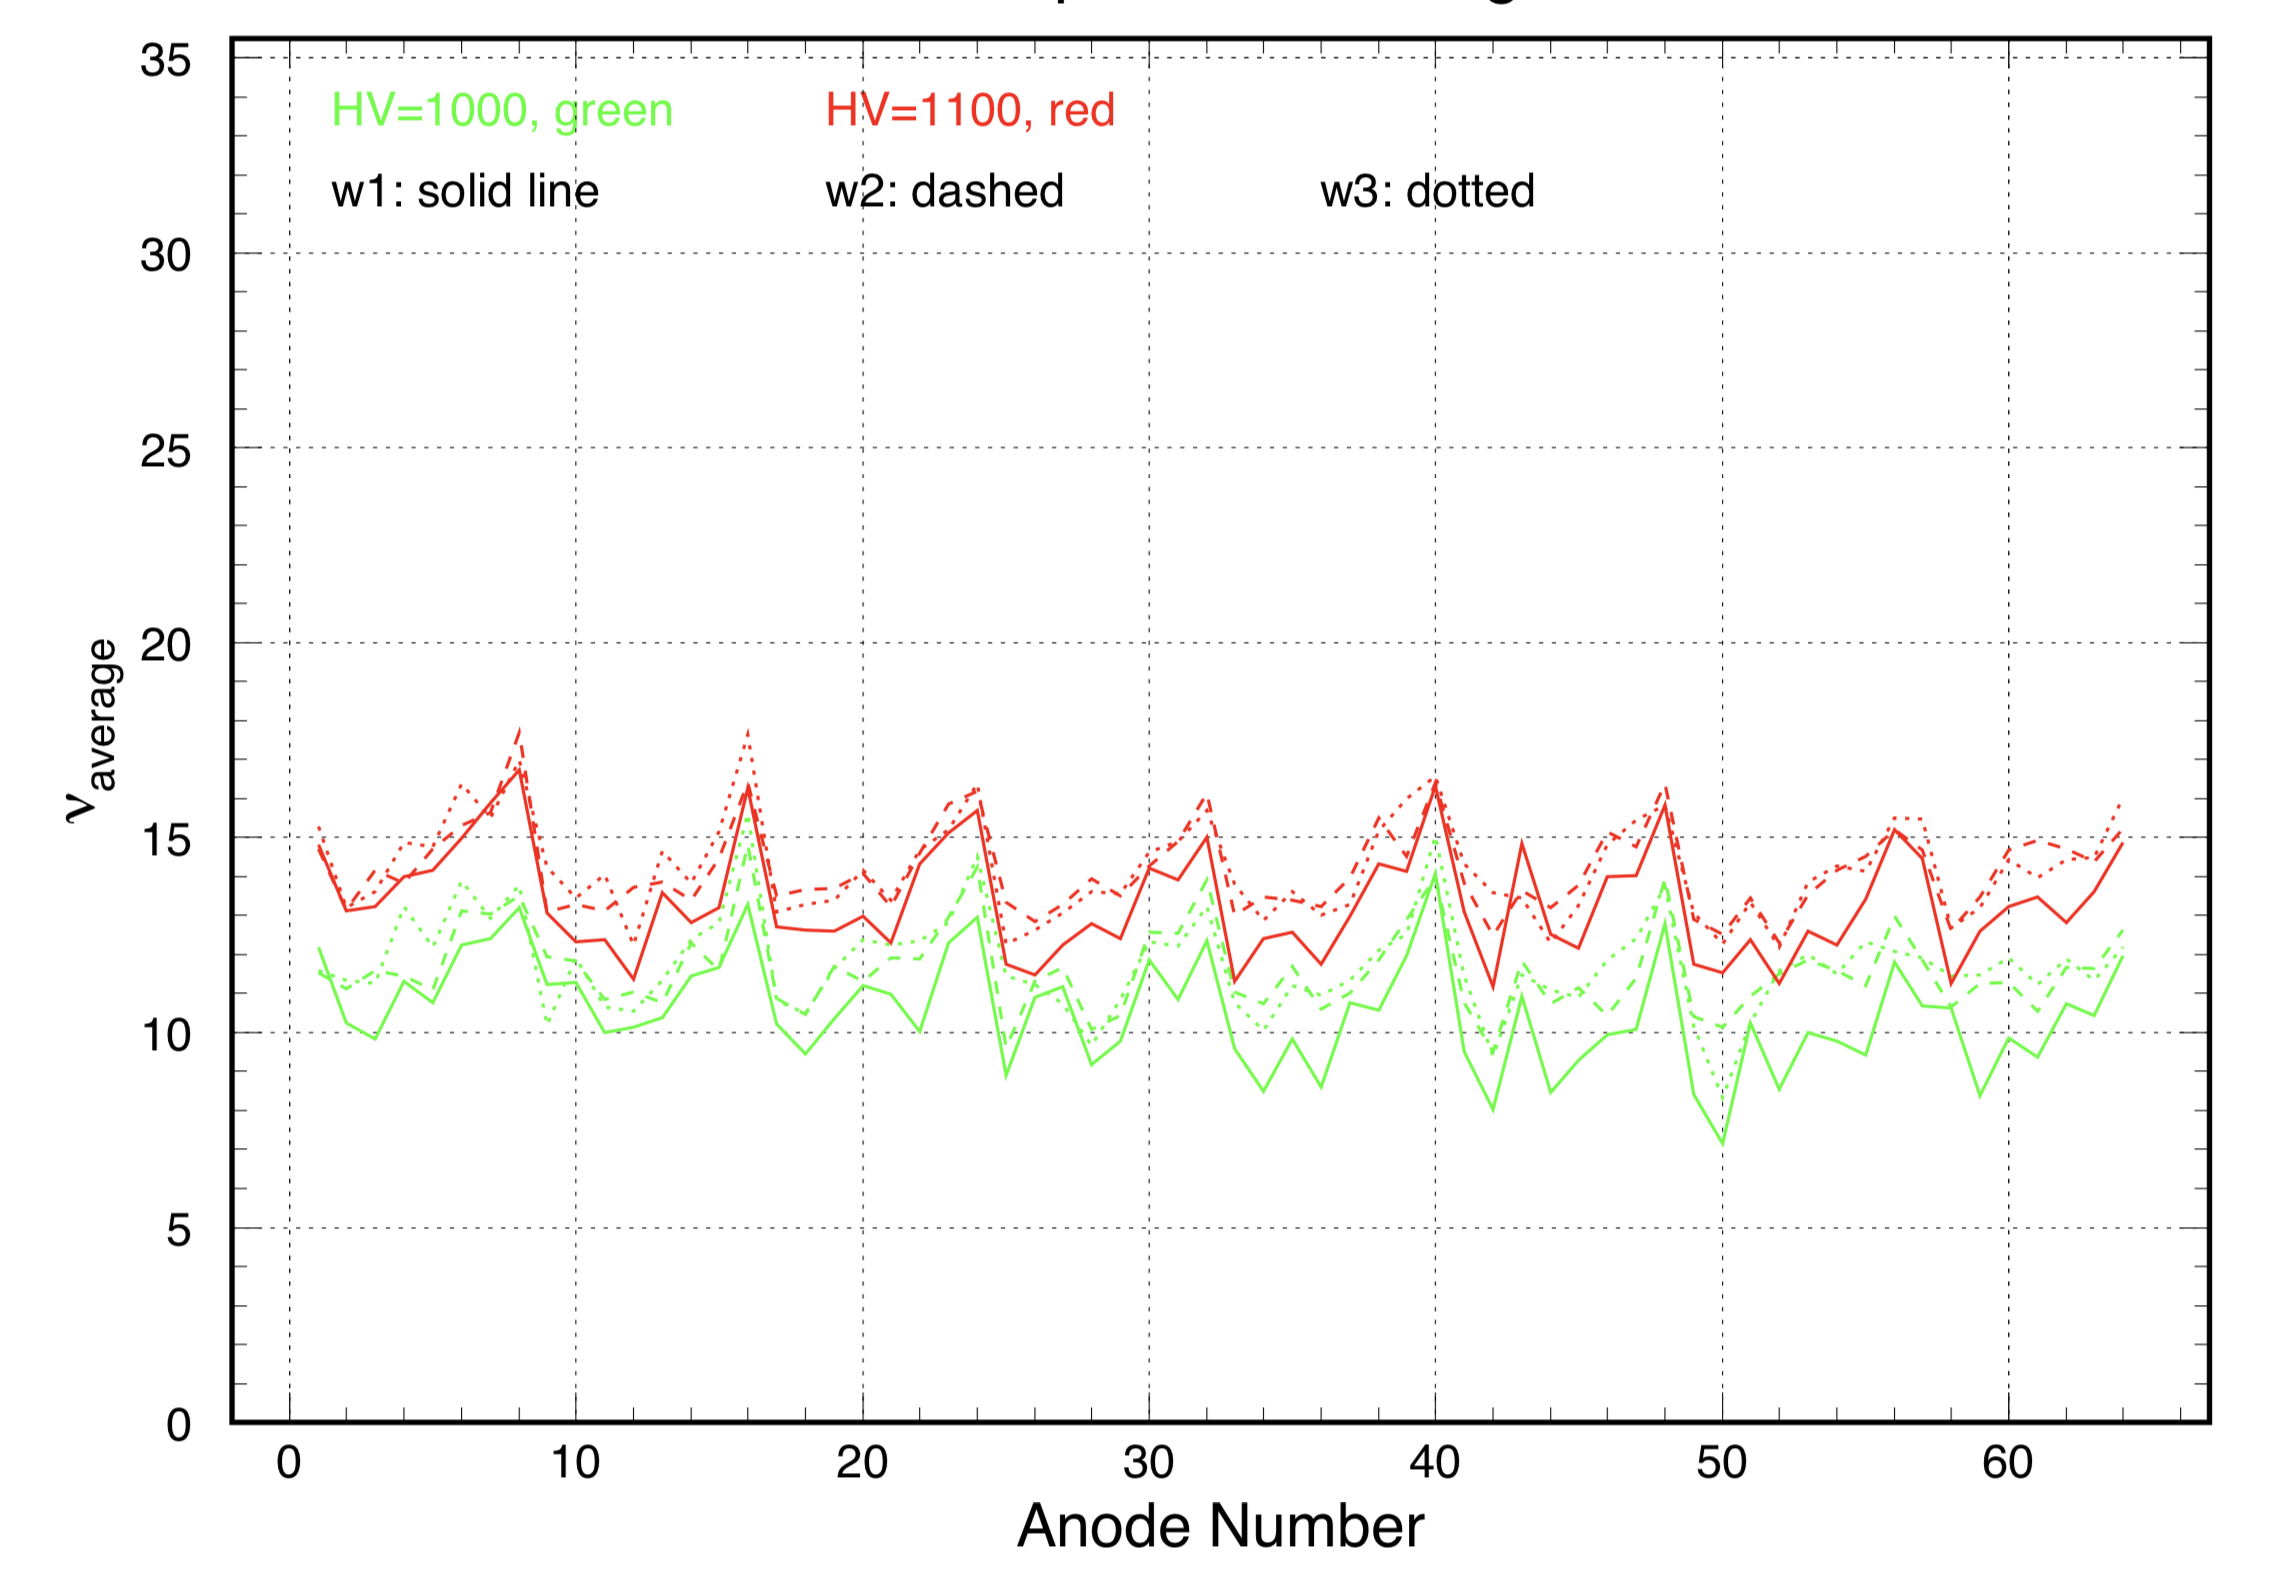
\includegraphics[width=0.95\linewidth]{H12700_nu.png}
	\caption{Distributions of fit parameters measured at 2 different high
          voltage supplies  (1000V and 1100V) and 3 different  light intensities (w1:w2:w3$\sim$100:10:1) for 64  pixels of one MaPMT: the parameter $scale$   characterizing
          the dynode amplification system (top), the average number of photoelectrons $\mu$ (center) and the first dynode amplification $\nu$ (bottom).}
	\label{fig:PavelPassport}
\end{center}
\end{figure}

The results of the characterization have been stored in the CLAS calibration database and are available for use in
the Monte Carlo simulations. The extracted gain values have been used to perform the equalization of all 25024
readout channels.

%\begin{figure}[ht]
%\begin{center}
%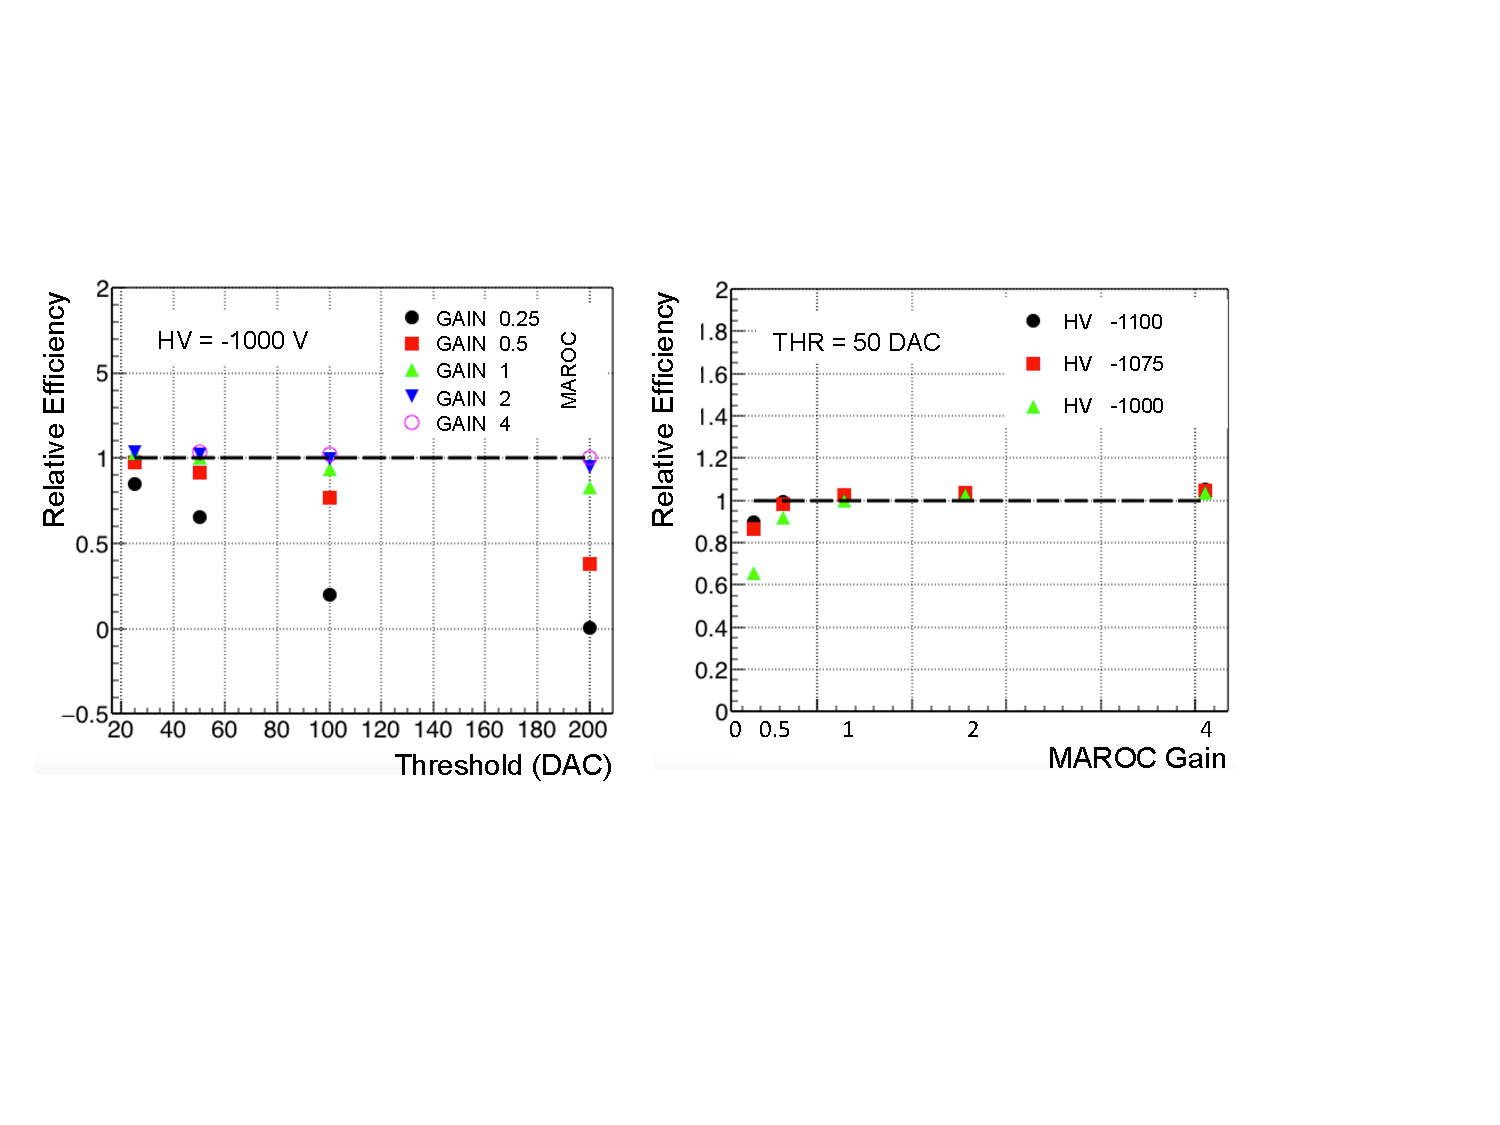
\includegraphics[width=1.0\columnwidth]{Figure4.pdf}
%\end{center}
%\caption{Relative SPE detection efficiency as a function of the working parameters: bias voltage,MAROC preamplification gain and discriminator threshold. The plots show the dependence %on two parameters while keeping fixed the third: bias voltage (left) or threshold (right). Data are normalized to the reference point at HV=-1000~V, gain=1 and threshold=+50 DAC. %Values greater than 1 are likely due to the cross-talk contribution.}
%\label{Fig:EfScan}
%\end{figure}

The dark noise SPE spectra allow for the study of the efficiency dependence on the working parameters, i.e. MaPMT
bias voltage, MAROC pre-amplification gain, and discriminator threshold \footnote{The programmed threshold
levels are expressed in Digital-to-Analog Converter (DAC) units, 1 DAC unit corresponds to about 1~mV.} using the
binary readout line. Data indicated that the efficiency reaches a plateau over a wide range of working parameter
values~\cite{Ref:RICHElectro}. %(see Fig.~\ref{Fig:EfScan}).
The plateau corresponds to the region where all of the MaPMT discharges  are digitized and the efficiency ultimately
depends on the quality of the photocathode. The plateau is a consequence of the saturated mode employed in the
MAROC binary readout and allows a flexible definition of the working point, a crucial feature when dealing with a large
number of channels in the challenging single-photon regime.

\clearpage

%-----------------------------------------------
\subsection{Services}
%-----------------------------------------------

The CLAS12 RICH requires various services, namely power, cooling, and gas purge whose number of lines has to be
minimized and installed outside of the CLAS12 acceptance. A continuous nitrogen flow, supplied by the Hall~B gas
distribution system, is provided in order to keep the relative humidity inside the RICH vessel at the few percent
level. The flow is set to about 60~l/m to ensure a complete inner volume exchange in a few hours. 
%The nitrogen is supplied by the Hall-B distribution system based on a large dewar filled of liquid nitrogen. 
A backup system has been realized by a stack of nitrogen bottles to allow for up to 3 days of gas flow in case of
failure of the primary distribution system.

The electronics power is controlled by a CAEN SY4527 power supply with five 8-channel A2518 low voltage (LV) boards and five
32-channel A1536 high voltage (HV) boards. Each LV channel powers 4 FPGA boards, while one HV channel drives one MaPMT. The
electronic readout is connected to the back-end by three MTP trunks of 2.5 Gbps optical fibers. One trunk groups
several multi-core fibers, each of them connecting one of the eight ports in the VME/SSP~\cite{daq-nim} back-end
module to four FPGA boards.

The readout electronics dissipates about 3.5~W per unit, mainly due to the FPGA chip and the optical transceiver, as
shown by the thermocamera image in Fig.~\ref{Fig:EleTile}. The total heat load, at the level of 500~W, is removed by
a forced air flow. Since the electronics panel is not fully sealed due to the numerous holes for the readout and HV
connectors, there is a diffusive exchange in the RICH vessel between the nitrogen gas used to keep the aerogel dry
and the air in the electronics panel. As a consequence, dry and clean air is required to cool down the electronics. This
is achieved with an Altas Copco multi-core oil free rotary scroll air compressor. The compressor fills a tank at 8~atm
pressure, from where the cooling air is filtered and circulated towards two distributors located at the sides of the
electronics panel and outside the acceptance. These are made of stainless steel tubes with several nozzles to direct
the cooling air supersonic flow along the board surface. The exhaust is made of six corrugated tubes that run in the
back of the RICH module behind the spherical mirror.

\begin{figure}[t]
\begin{center}
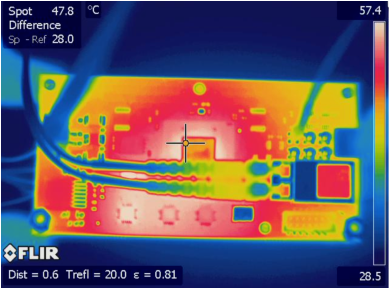
\includegraphics[width=0.90\columnwidth]{FPGA_heat.pdf}
\end{center}
\caption{The CLAS12 RICH readout unit as imaged by a thermocamera. The hottest spots are the FPGA chip in the
  center and the optical transceiver on the right.}
\label{Fig:EleTile}
\end{figure}

%-----------------------------------------------
\section{Assembly and Installation of the Detector}
%-----------------------------------------------

The assembly of the RICH detector was performed in a clean room and each element was installed after the completion
of the relative characterization tests. The trapezoidal RICH vessel was attached to a large aluminum structure with a
pivot to rotate the detector from the vertical to the horizontal position, as required by the various assembly phases.

%This assembly phase included also a detailed survey of the position and alignment
%of each inner element, in particular the mirrors, with respect to the mechanical structure of the detector.
The ten spherical sub-mirrors were mounted on a common frame inside the RICH vessel. To
minimize the material budget, the frame is composed by a net of 1.5-mm-thick carbon-fiber U-profiles. Each element
(frame and sub-mirrors) has three mounting points designed to allow precise alignment. The relative alignment of
the sub-mirrors was performed with the same setup used to determine their surface accuracy. The full spherical
mirror was illuminated by a point-like source and the position of each sub-mirror was adjusted until the ten spot images
converged into the nominal center of curvature. In Fig.~\ref{fig:MirSpots}, the reflected images before the alignment
(when each sub-mirror produces a spot at a different location) and after the alignment (when all the spots overlap
within a few mm) are shown. The quality of the result is also visible in Fig.~\ref{fig:MirAlign}, where the spherical
mirror system before (left) and after (right) the alignment is shown.

\begin{figure}
\begin{center}
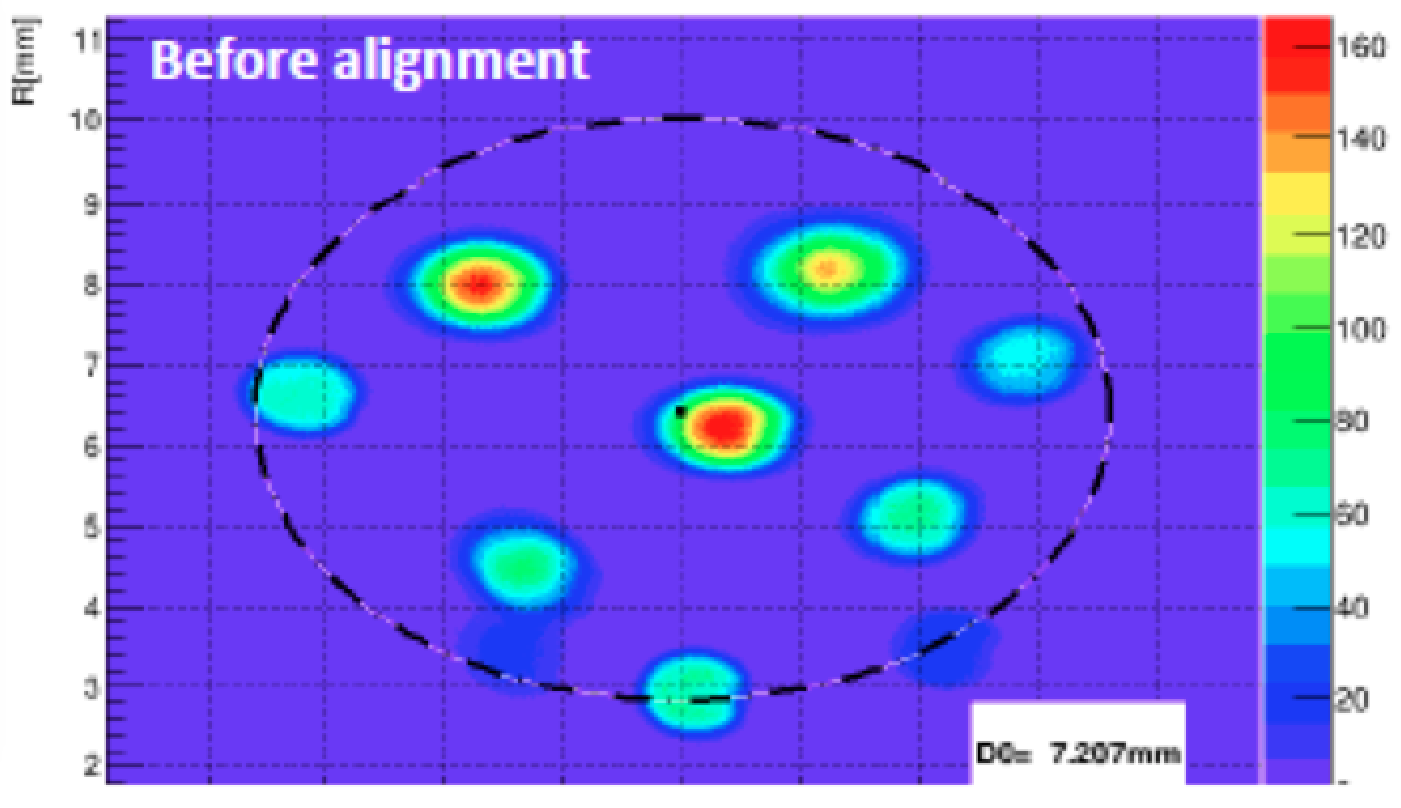
\includegraphics[width=0.50\textwidth]{mirror_spot1.png}
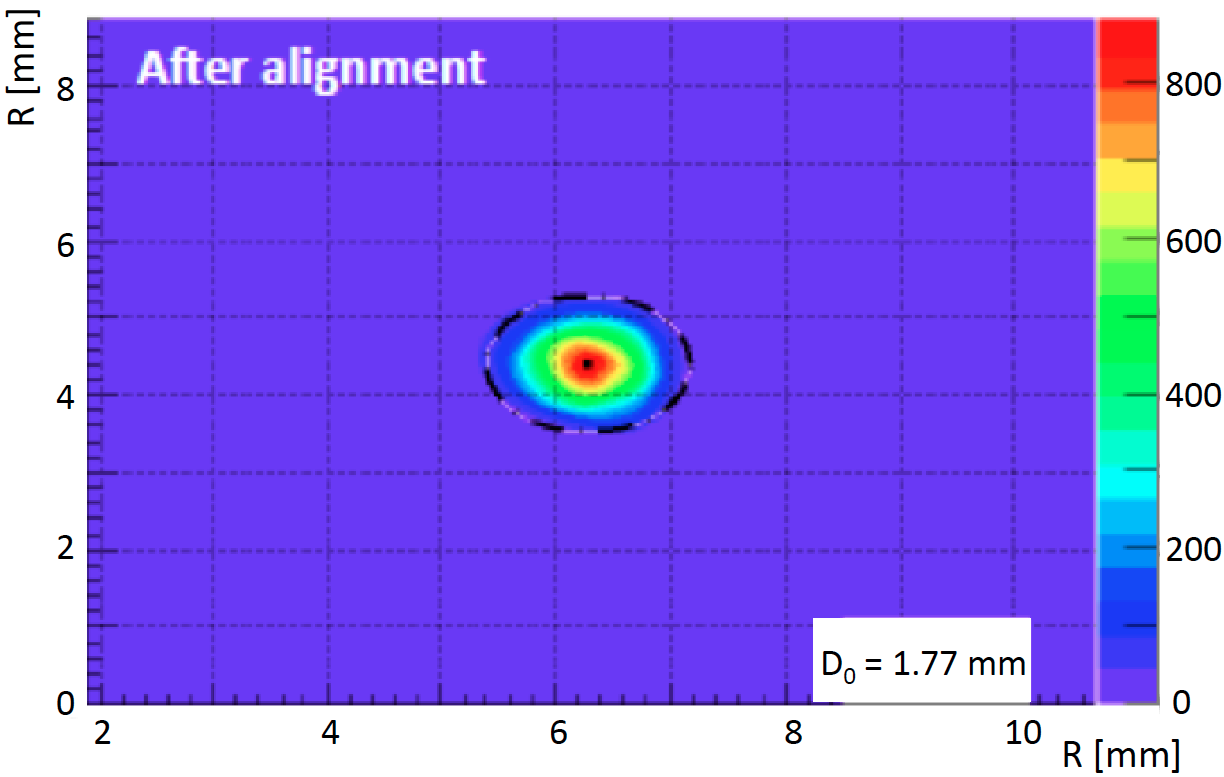
\includegraphics[width=0.50\textwidth]{mirror_spot2.png}
\caption{Reflected spot by the whole spherical mirror system: before the alignment (top plot), all sub-mirrors
  image the light source in different locations; after the alignment (bottom plot), all images overlap in the same
  position. The spot brightness depends on how close the sub-mirror center is to the sensor position.}
\label{fig:MirSpots}
\end{center}
\end{figure}

\begin{figure}
\begin{center}
\includegraphics[width=0.50\textwidth]{mirror_before.png}
\includegraphics[width=0.50\textwidth]{mirror_after.png}
\caption{The spherical mirror before (top plot) and after (bottom plot) alignment. As a result of the alignment, the image
  appears continuous along the whole mirror surface.}
\label{fig:MirAlign}
\end{center}
\end{figure}

The lateral and bottom planar mirrors were attached to the RICH trapezoidal vessel structure by means of
joints allowing a precise alignment. The two frontal mirrors
were mounted on the lower frontal panel made of carbon-fiber. The relative position of the mirrors was
aligned with respect to the RICH vessel at the level of about 0.5~mrad by using a faro-arm. The fully installed
mirror system as seen from the entrance panel is shown in Fig.~\ref{fig:mirrors}.

\begin{figure}
\begin{center}
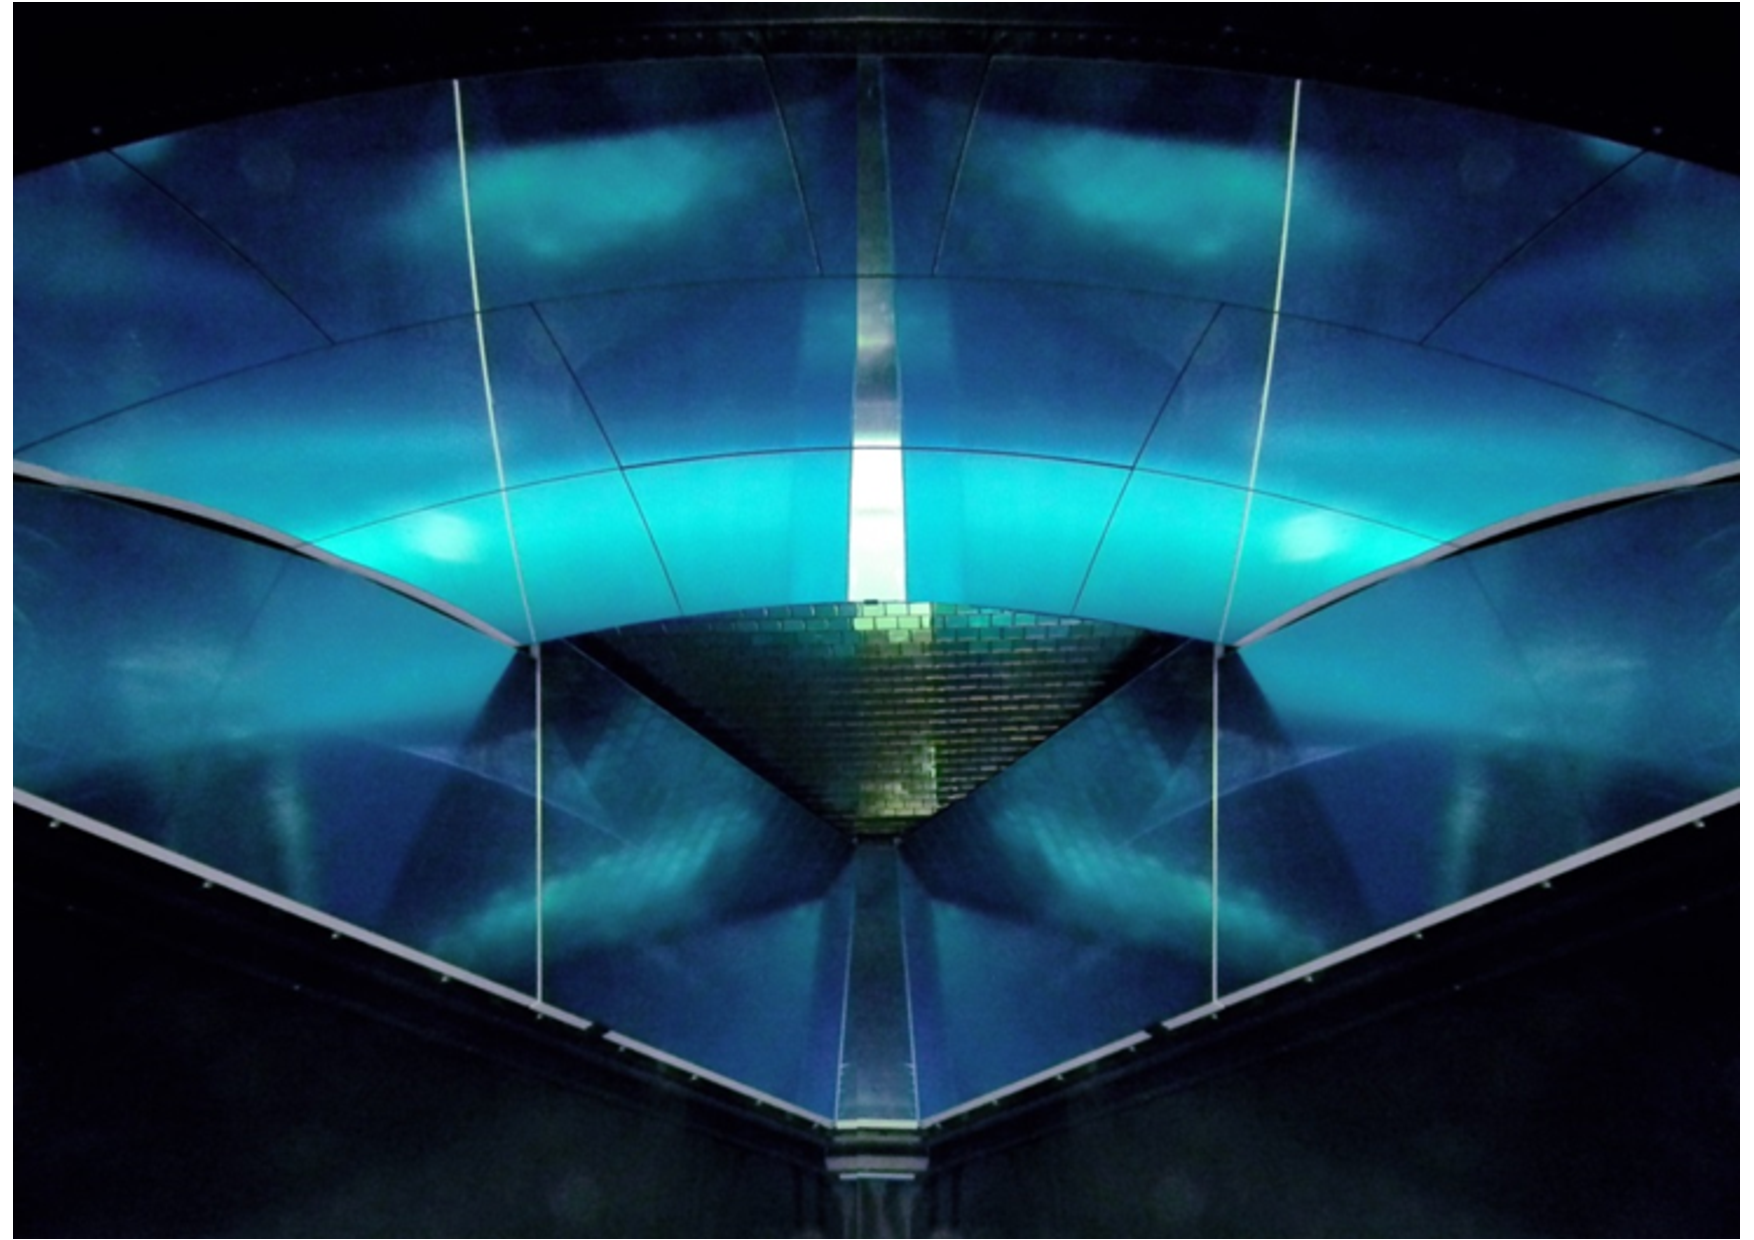
\includegraphics[width=0.50\textwidth]{mirrors.pdf}
\caption{The mirror system as it is seen from the RICH entrance panel. Clockwise from the top, the ten spherical
  sub-mirrors, the two right lateral mirrors, the bottom mirror, and the two left lateral mirrors are visible. At the
  center, the MaPMT array is also visible.}
\label{fig:mirrors}
\end{center}
\end{figure}

The RICH photon detectors and readout electronics were installed on the electronics panel using an independent
aluminum support structure to enable easy access and to allow rotations during the functionality tests. The PMTs
with higher gain were placed closer to the beam pipe, where better detection performance is required. As the \MaPMT in
one readout unit share the same HV bias, they were selected of similar gain and same type (H8500 or H12700).
The fully equipped electronics panel is shown in Fig.~\ref{fig:MaPMTs} from the MaPMT side and in
Fig.~\ref{fig:electronics} from the readout electronics side.

\begin{figure}
\begin{center}
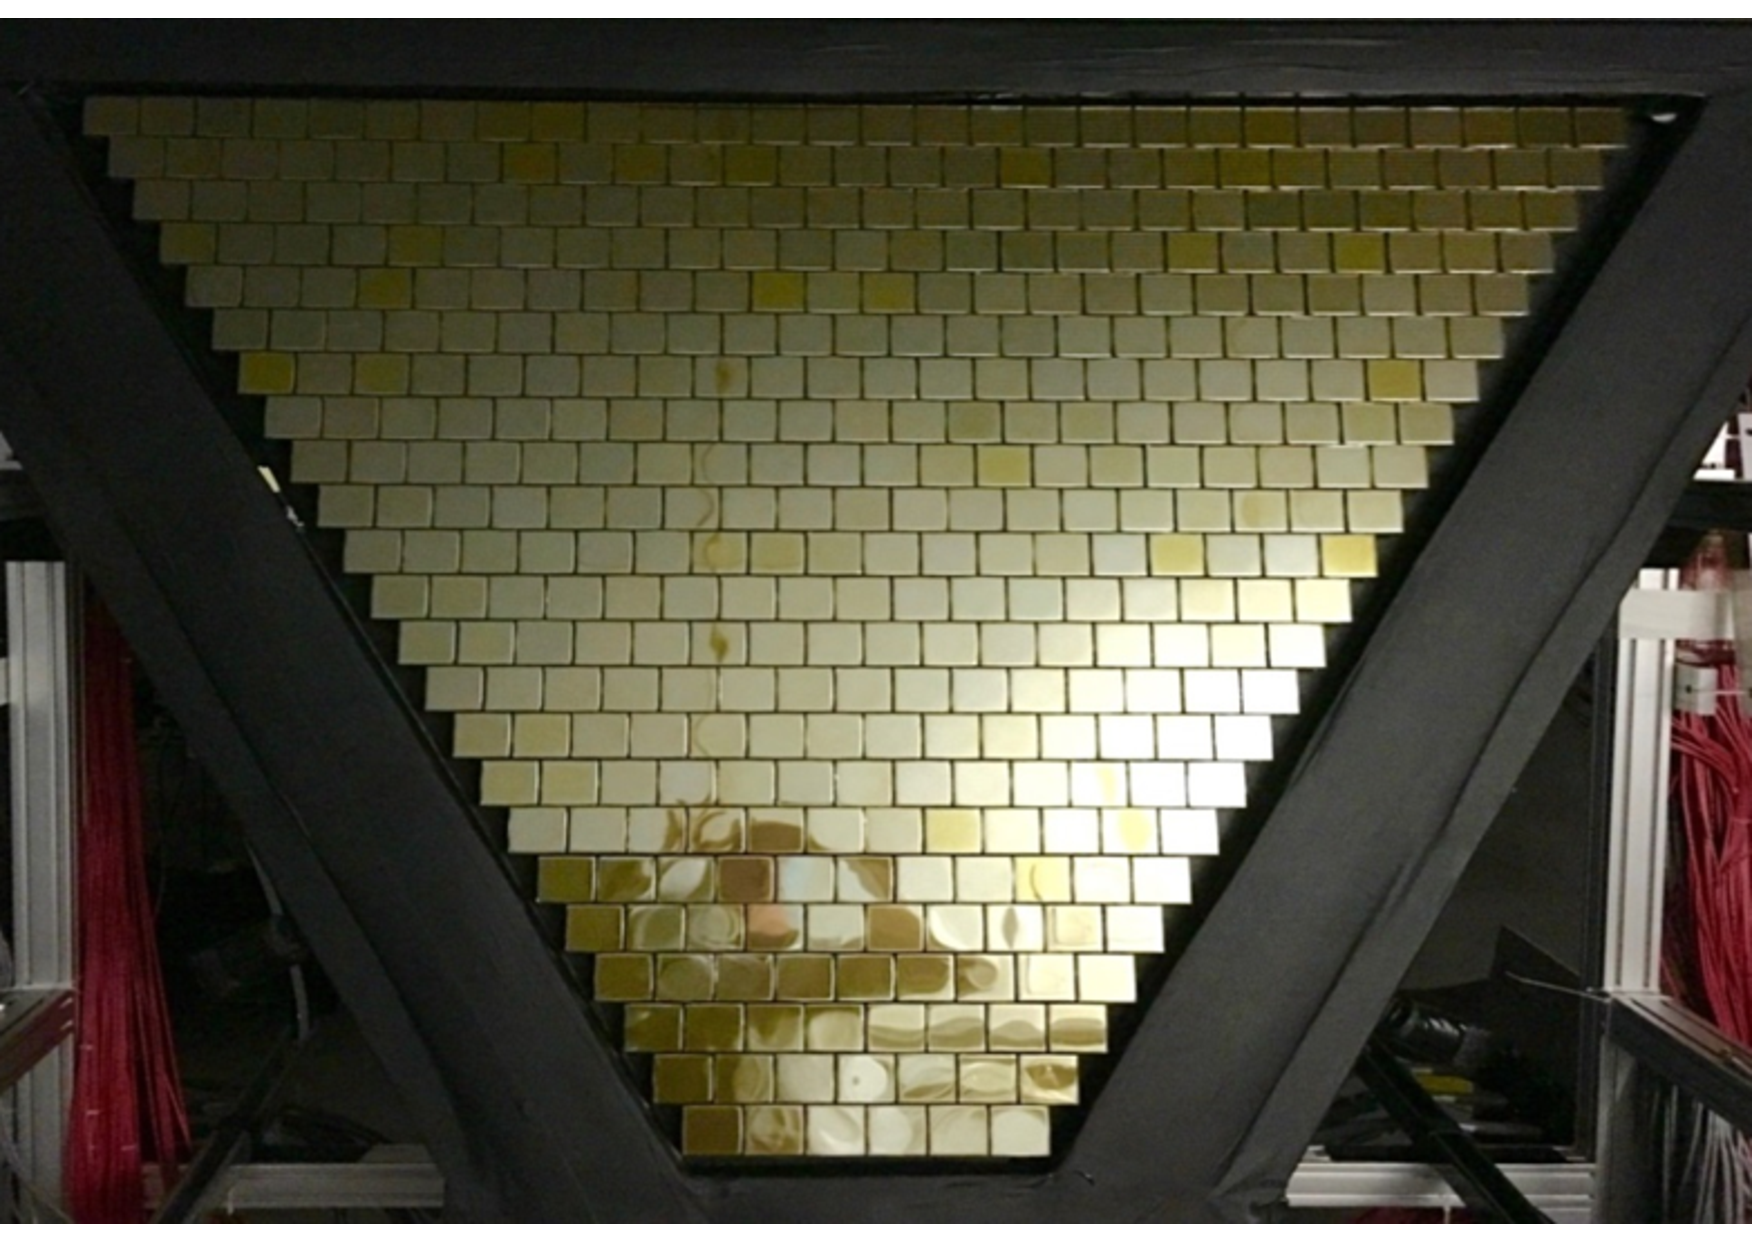
\includegraphics[width=0.50\textwidth]{MaPMT.pdf}
\caption{The fully assembled plane of MaPMTs.}
\label{fig:MaPMTs}
\end{center}
\end{figure}

\begin{figure}
\begin{center}
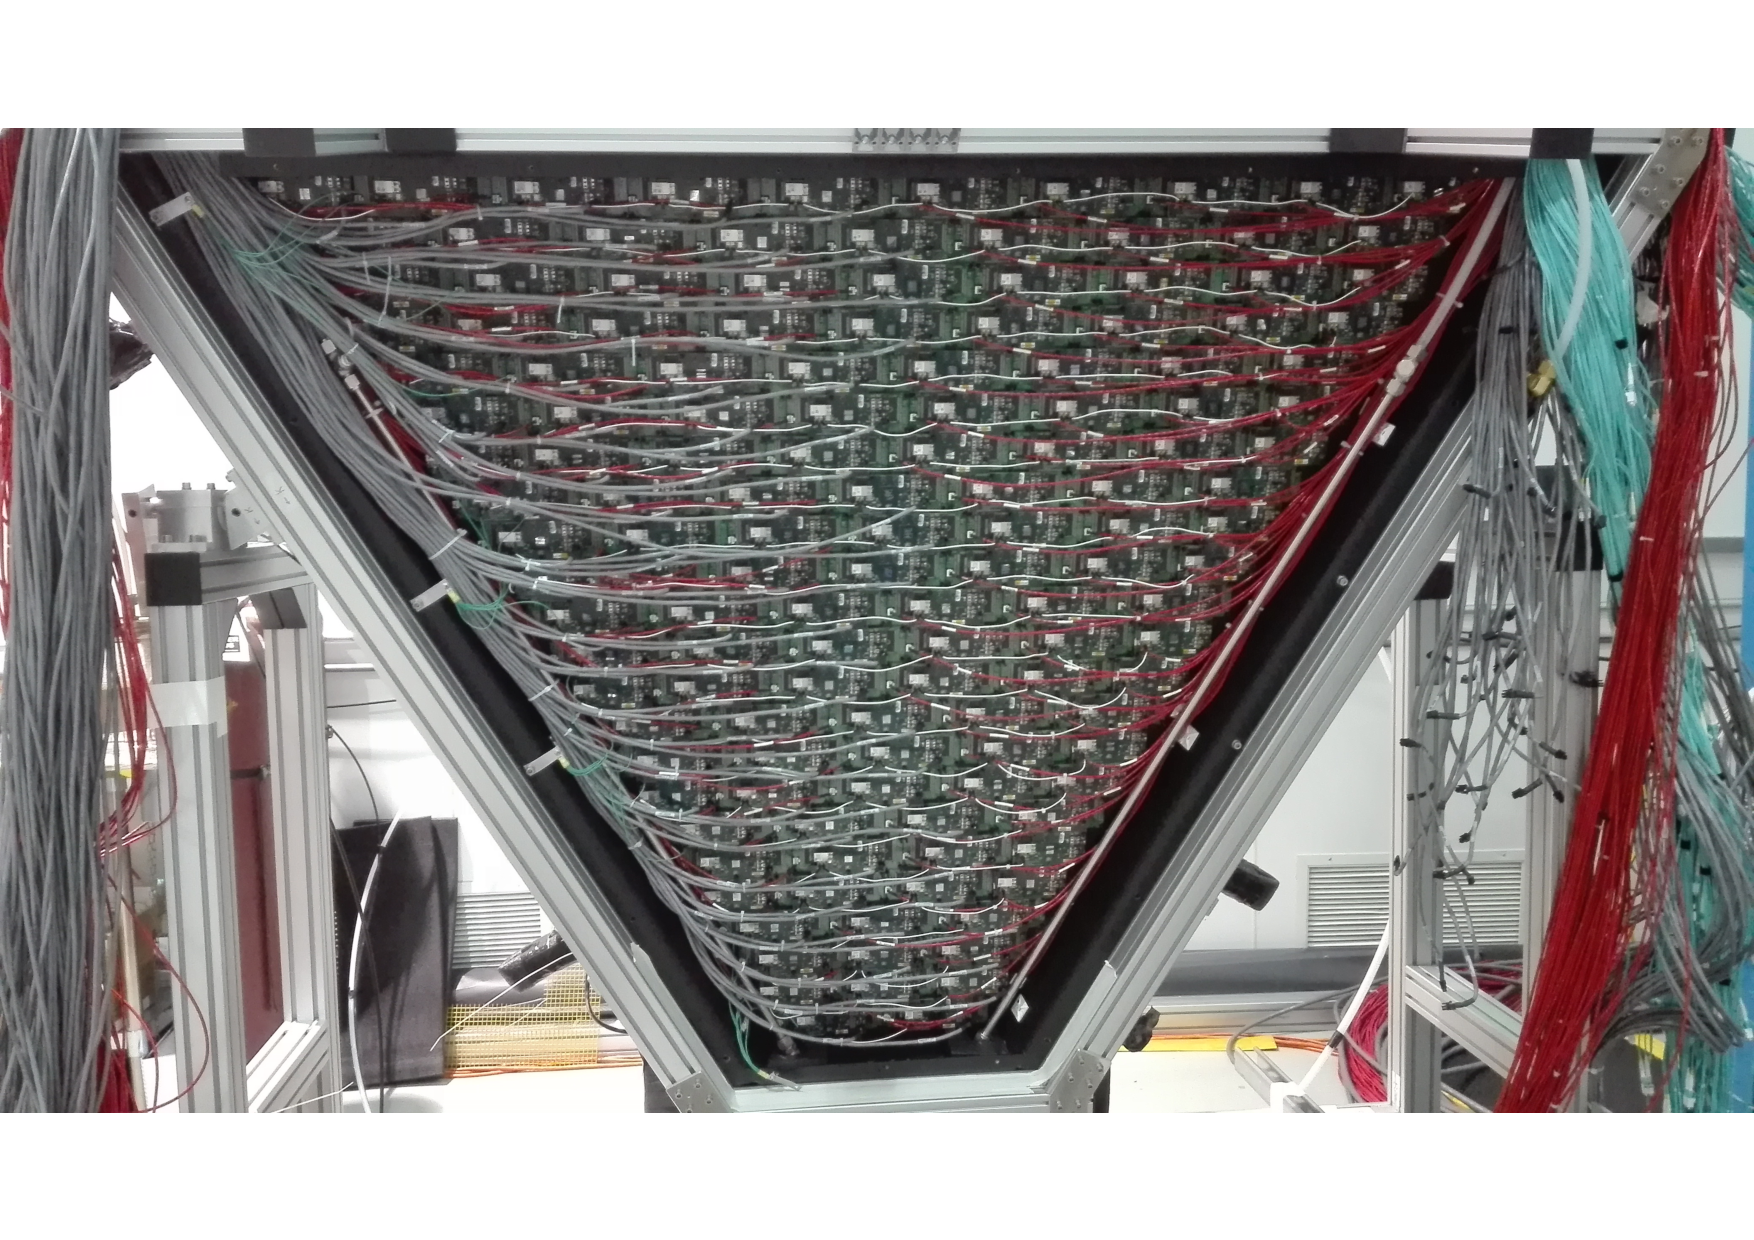
\includegraphics[width=0.50\textwidth]{electronics.pdf}
\caption{The fully assembled and cabled front-end electronics. Visible are the gray 20 AWG LV cables, the red
  HTC-50-1-1 HV cables, and the cyan MTP optical fibers.}
\label{fig:electronics}
\end{center}
\end{figure}

After the electronics panel assembly was completed, particular care was devoted to minimize and stabilize the
pedestal width values. The measured pedestal RMS was initially at the level of few DAC units, with relatively large
variations not only from MaPMT to MaPMT but also among the channels of a single MaPMT, as shown in the top
plot of Fig.~\ref{fig:GroundG}. As the readout uses a single threshold value per chip (or MaPMT), the channel by
channel variation may effect the single channel efficiency in a way that  would be complicated to correct for.
Therefore, a grounding grid was realized by connecting all of the boards to the detector chassis with a copper wire.
In this way, all of the components of the readout system, powered by the floating 5~V low-voltage lines, were properly
referred to the same ground. This reduced the typical pedestal RMS down to about 1 DAC unit, a level comparable
with the test bench results, as shown in the bottom plot of Fig.~\ref{fig:GroundG}.

\begin{figure}[t]
\begin{center}
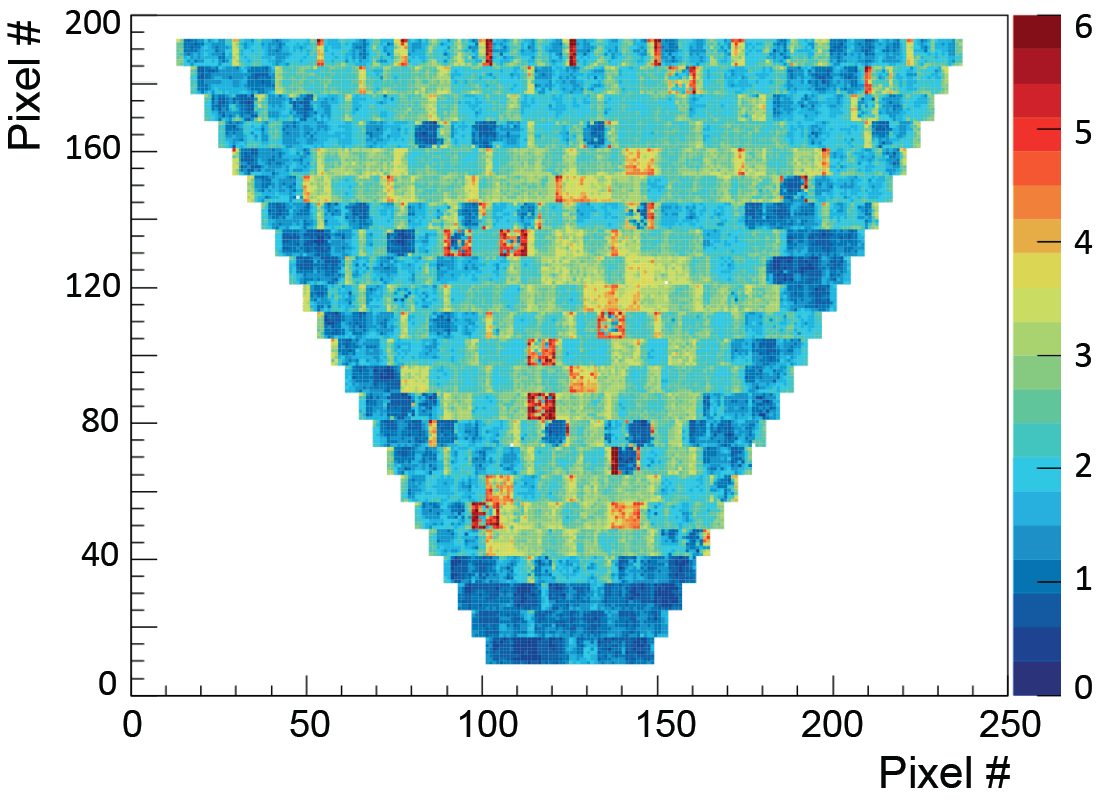
\includegraphics[width=1.0\columnwidth]{pedestal_rms_before.png}
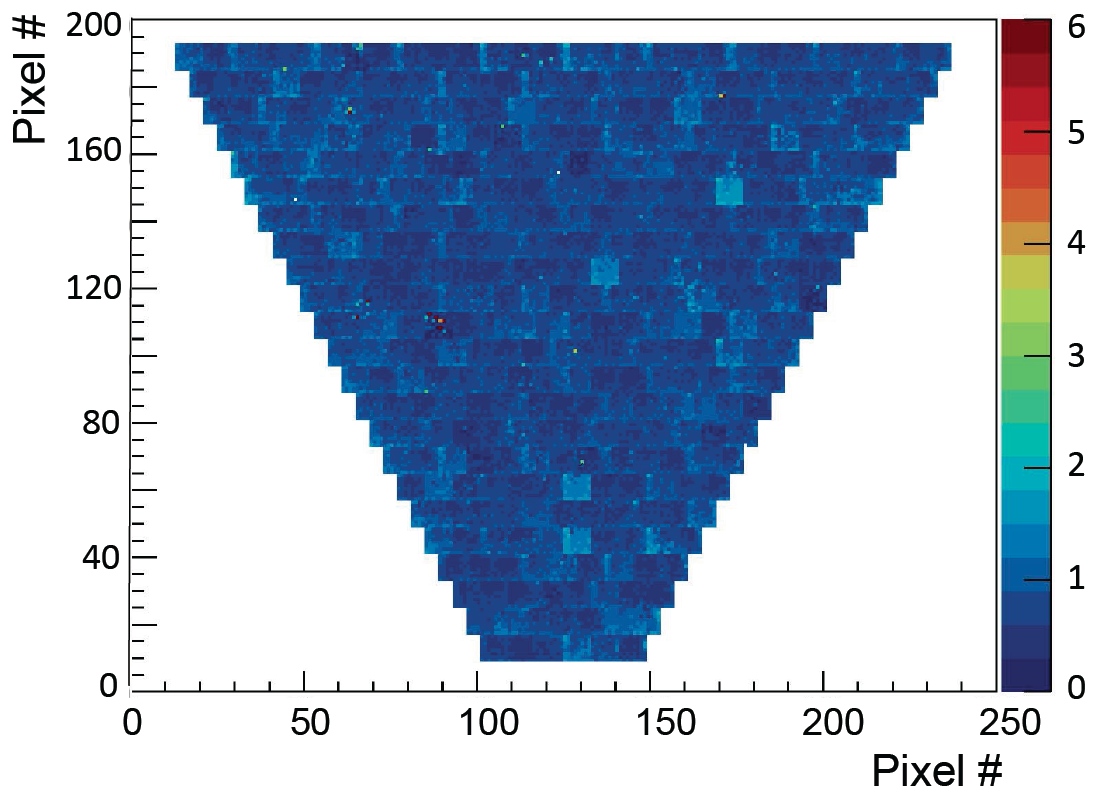
\includegraphics[width=1.0\columnwidth]{pedestal_rms_after.png}
\end{center}
\caption{Map of the pedestal RMS values before (top) and after (bottom) the realization of a grounding grid
  connecting all of the electronics units to the RICH chassis to provide a common ground reference for the floating
  power lines.}
\label{fig:GroundG}
\end{figure}

Several tests were performed at various stages of the electronics assembly, using cosmic rays.
%detected by a tracking system installed on a dedicated trigger station inside a large dark box. 
%The set up used was composed of a large dark box and two plastic scintillators positioned on the top and bottom to define the cosmic ray trajectory. The Cherenkov light generated by an aerogel tile placed inside the box was detected by the electronic panel also placed Inside the box.
In the absence of a precise measure of the cosmic particle momentum, it was not possible to perform any study of
the Cherenkov angle resolution. Nevertheless, cosmic runs allowed for the validation of the translation tables relating
the electronics channels to the pixel positions, the development of the ring reconstruction software, the verification of
the stability of the system, and the testing of the performance of the power supplies, cooling, readout, slow controls,
and interlock services. After all planned tests were completed, the complete readout system was eventually transferred
into the mechanical structure.

%and the closing panels temporarily mounted. The backward side of the RICH was then completed by installing the upper exit panel.
The aerogel was the last element installed, being the most sensitive to the external conditions. For this reason, before
its assembly, a test to verify the gas-tightness of the RICH vessel, temporarily completed with all of the closing panels,
was performed. Each aerogel tile was inspected and mounted in a pre-selected location of the supporting structure,
namely the frontal mirrors for the 2~cm tiles and the upper frontal panel for the 3~cm tiles. The location of
each tile was determined in order to concentrate the tiles with the higher expected photon yield at forward polar
angles where the particle identification requirements are most demanding. In addition, tiles with close optical
properties were coupled in the same location of the double 3~cm layer. The tiles were secured in place by a net of
nylon wires that ran along the edges and, on the side, by plastic bumpers covered by a thin foam layer to avoid
damage to the aerogel. The tiles were also optically isolated from each other by using a thin layer of foam stretched around
each tile. In fact, photons produced in one tile and propagating through an adjacent tile undergo surface effects that
generally degrade the angular resolution. The foam is instrumental to avoid sharp edge contacts between the blocks
that might originate cracks in the aerogel material. In addition, the foam net bonds the tiles together in forming a sole
and stable layer. Figure~\ref{Fig:AeroB1} shows the frontal planar mirror system with the aerogel tiles fully installed.

During the assembly, the aerogel panels were maintained in a low-humidity atmosphere (around 20\% relative humidity)
to prevent moisture absorption. Once the assembly of all tiles was completed, the panels were quickly installed on
the RICH vessel, the detector was sealed with all of the closing panels and a flow of purged nitrogen was started to
minimize the exposure to the external weather conditions.

\begin{figure}
\begin{center}
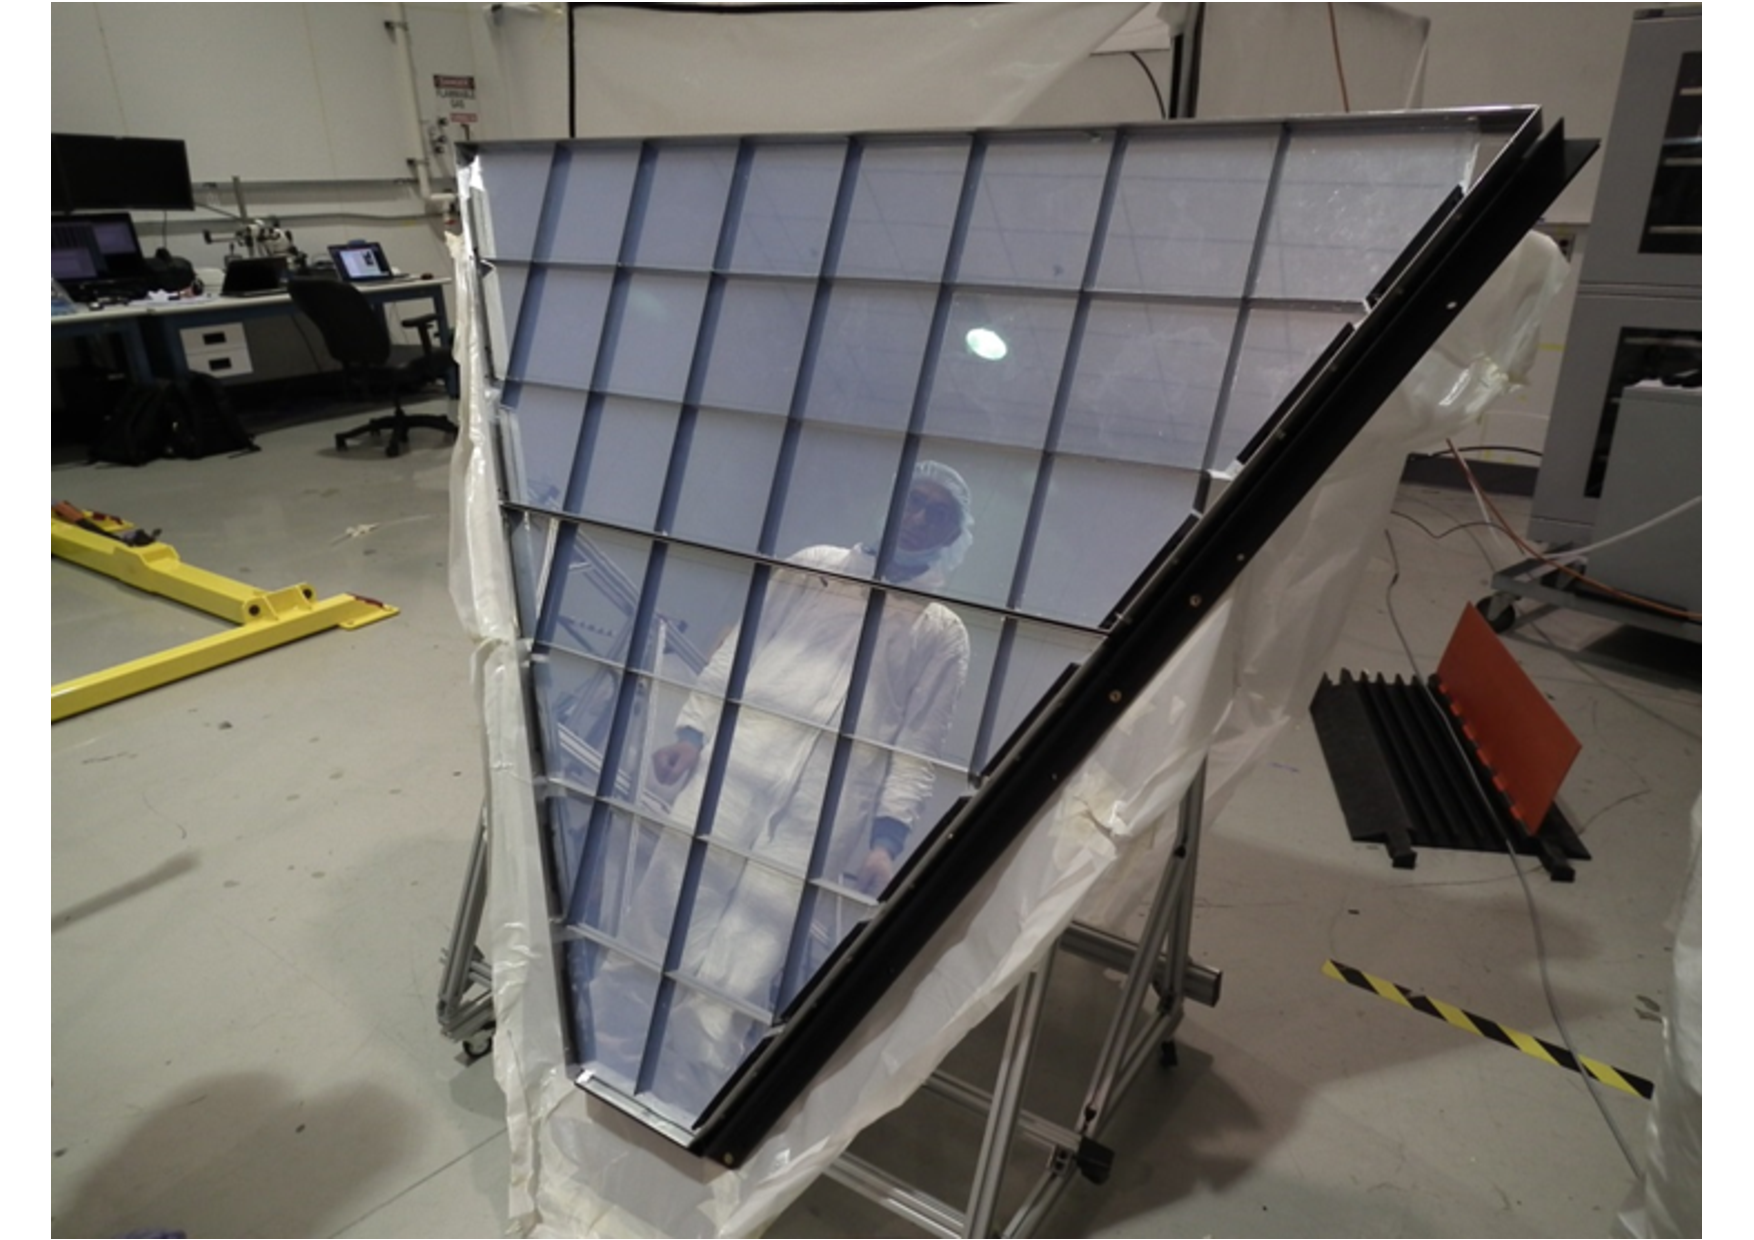
\includegraphics[width=0.45\textwidth]{aerogel_bottom.pdf}
\caption{The 2-cm-thick section of the aerogel mounted on the two RICH frontal mirrors. Visible are the
  external aluminum frame and the black foam net that optically and mechanically isolates each tile from the others.}
\label{Fig:AeroB1}
\end{center}
\end{figure}

Once the detector was sealed and before the transportation to the experimental hall, its functional parameters were
tested for several weeks in the assembly room. The tests included the two gas systems serving the RICH: the nitrogen
system that must keep the internal humidity at the few percent level to preserve the aerogel optical performance and
the air cooling system of the readout electronics.

\begin{figure}[t]
\begin{center}
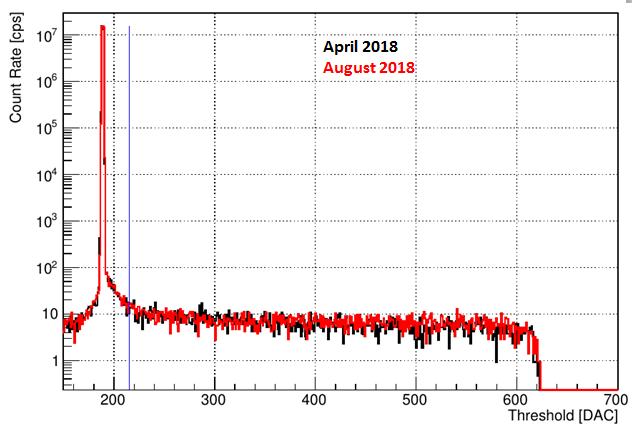
\includegraphics[width=1.0\columnwidth]{SPEdark.png}
\end{center}
\caption{Example of a SPE spectrum from the dark rate measurement of one readout channel as a function of the
  threshold value. The two histograms were recorded in April and August 2018. The blue line indicates the threshold
  setting.}
\label{fig:SPEdark}
\end{figure}

\begin{figure}[t]
\begin{center}
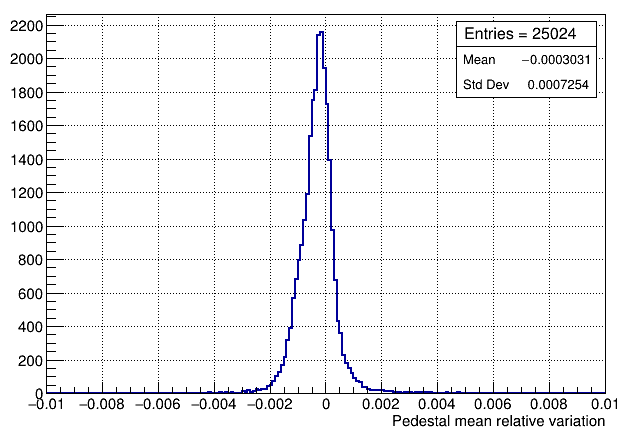
\includegraphics[width=1.0\columnwidth]{PedestalMeanVariation.png}
\end{center}
\caption{Relative variation of the mean pedestal position of the 25024 readout channels between April and August
  2018.}
\label{fig:PedestalMean}
\end{figure}

%-----------------------------------------------
\section{Commissioning of the Detector}
%-----------------------------------------------
\label{sec:Commissioning}

The RICH detector was installed in the CLAS12 spectrometer at the beginning of January 2018, in time with the start
of the data taking in Hall~B. In preparation for the data taking, a number of tests were routinely performed without
and with beam to establish the running conditions and to verify the stability of the response.


\begin{figure}[t]
\begin{center}
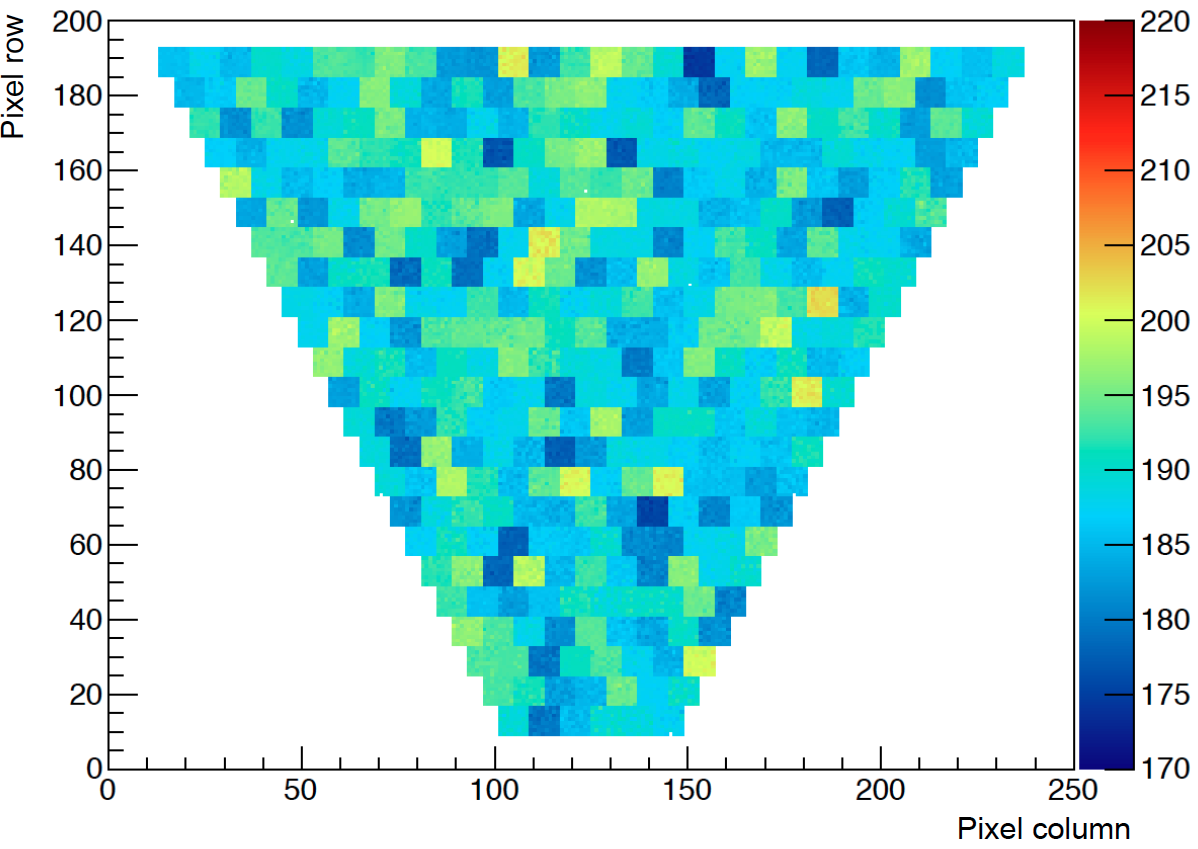
\includegraphics[width=1.0\columnwidth]{Pedestal_map.png}
\end{center}
\caption{Map of the mean pedestal position in DAC units (color scale).}
\label{fig:PedestalMap}
\end{figure}

\begin{figure}[t]
\begin{center}
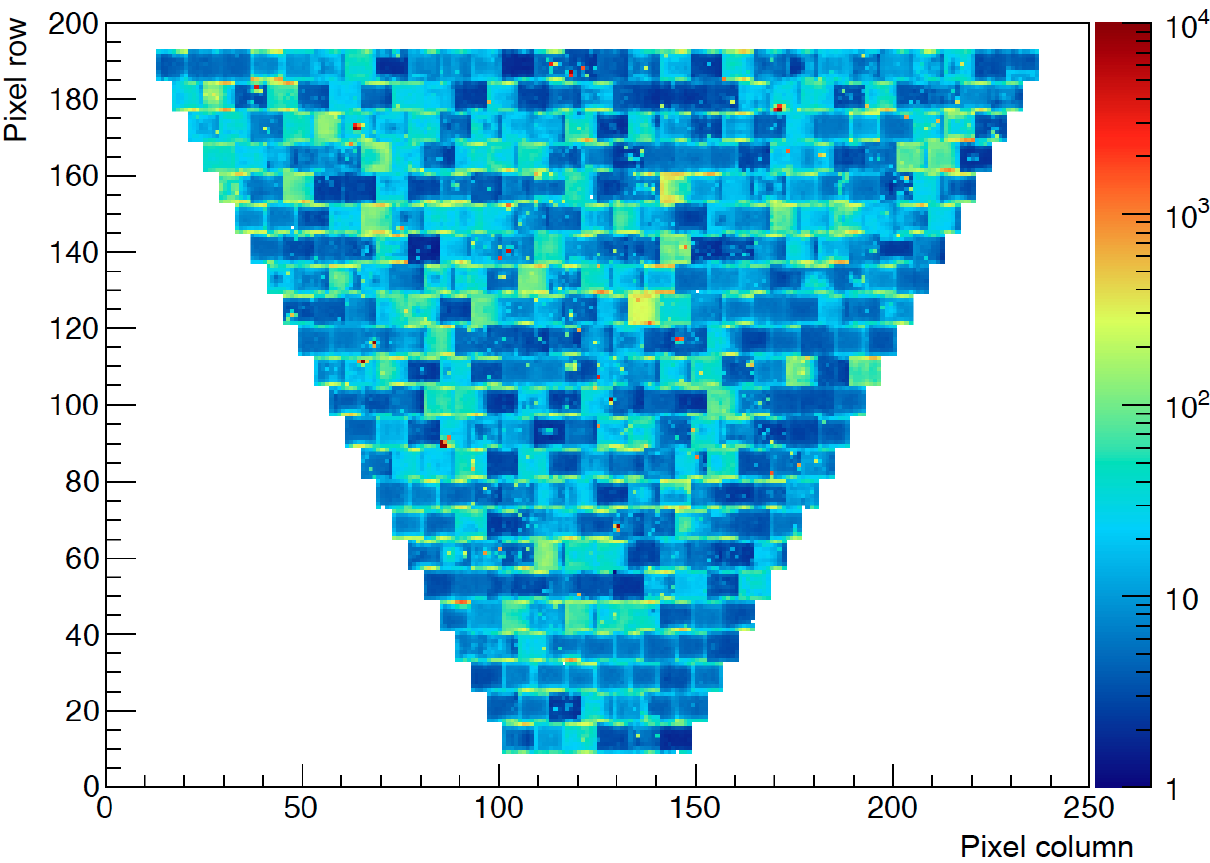
\includegraphics[width=1.0\columnwidth]{Darkcount_map.png}
\end{center}
\caption{Map of the average dark count rate in the plateau region of threshold values (color scale).}
\label{fig:DarkCountMap}
\end{figure}


The basic tool to monitor the RICH front-end electronics is provided by the measurement of the MaPMT dark noise
counting rate using the self-triggered scaler readout provided by the FPGAs. The number of counts above a programmed
threshold is recorded for a time on the order of a second. A fine scan of the threshold value allows for the
reconstruction of the full SPE spectrum for each of the 25k channels. An example of one SPE spectrum is shown in
Fig.~\ref{fig:SPEdark}. The main features of the data are: {\it{a)}} a very narrow pedestal where the threshold equals
the baseline,  {\it{b)}} a region close to the pedestal where the rate smoothly decreases as the threshold increases
(corresponding to the almost linear regime of the MAROC), and  {\it{c)}} a large plateau of the saturation regime, where
the count rate is basically insensitive to the threshold setting almost up to the edge of the SPE region. The plateau is a
crucial feature of the front-end electronics, because it allows a flexible definition of the working point without the need
for extreme precision in the channel equalization. The spectra allow for the channel-by-channel extraction of the 
pedestal position and width, the dark count rate in the plateau region, and the amplitude of the SPE region. The black
and red histograms in Fig.~\ref{fig:SPEdark}, taken in April and August 2018, respectively, demonstrate the stability
of the readout system over several months of running. Moreover, in Fig.~\ref{fig:PedestalMean}, the relative variation
of the mean pedestal position in the same interval of time is shown. On average, the pedestals are stable at the level of
$10^{-3}$.

The pedestal level is different for each readout channel, but it is quite uniform within one MAROC chip, as can be
seen from the map shown in Fig.~\ref{fig:PedestalMap}. This result guarantees the effectiveness of the common
threshold.

The average count rate in the plateau region provides a measurement of the dark count rate of the channel, as shown
in the map of Fig.~\ref{fig:DarkCountMap}. The typical dark count rate is a few tens of Hz, with more than 99\% of
the channels below 100~Hz and only few channels above 10~kHz. It is also found that the highest dark count rates in
the MaPMTs are located in the first and last row of pixels. Although measured with a completely different setup,
these results are in good agreement with the values quoted in the Hamamatsu data sheets.

\begin{figure}[t]
\begin{center}
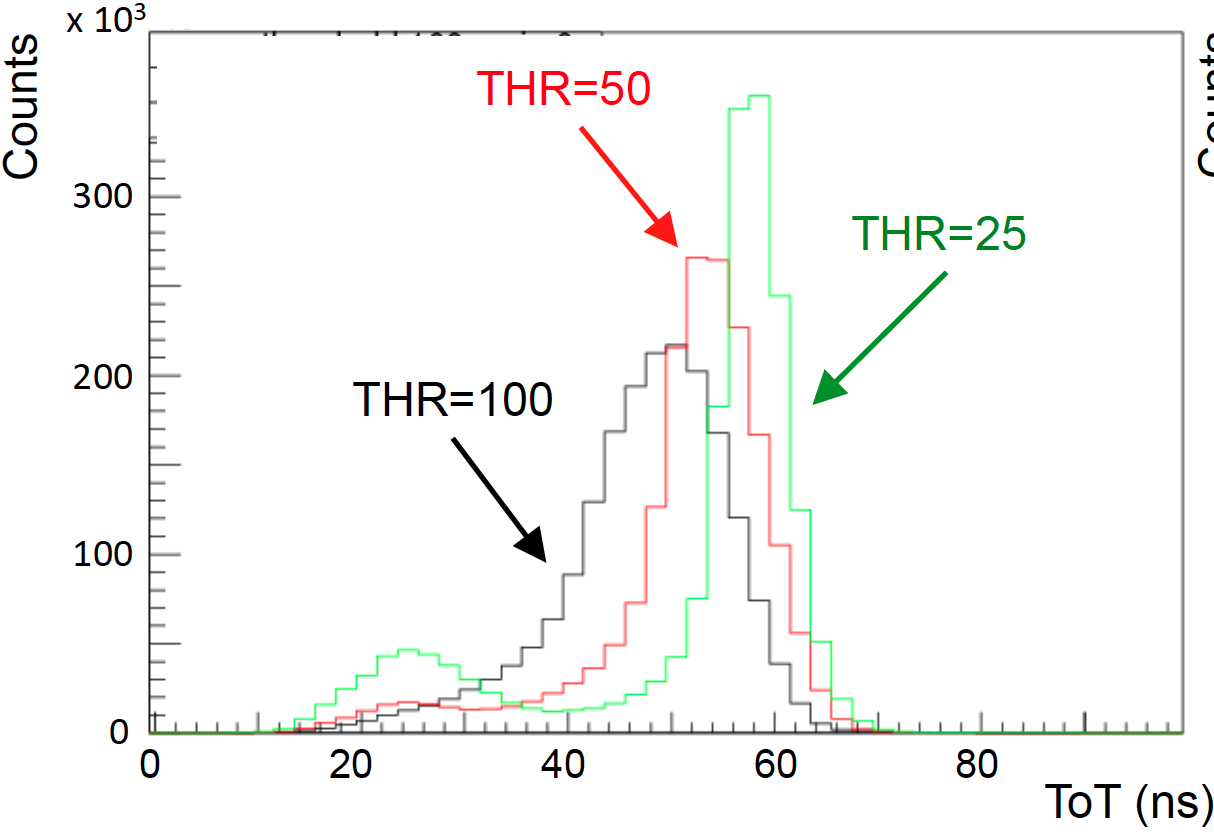
\includegraphics[width=0.95\columnwidth]{Equalize_before.png}
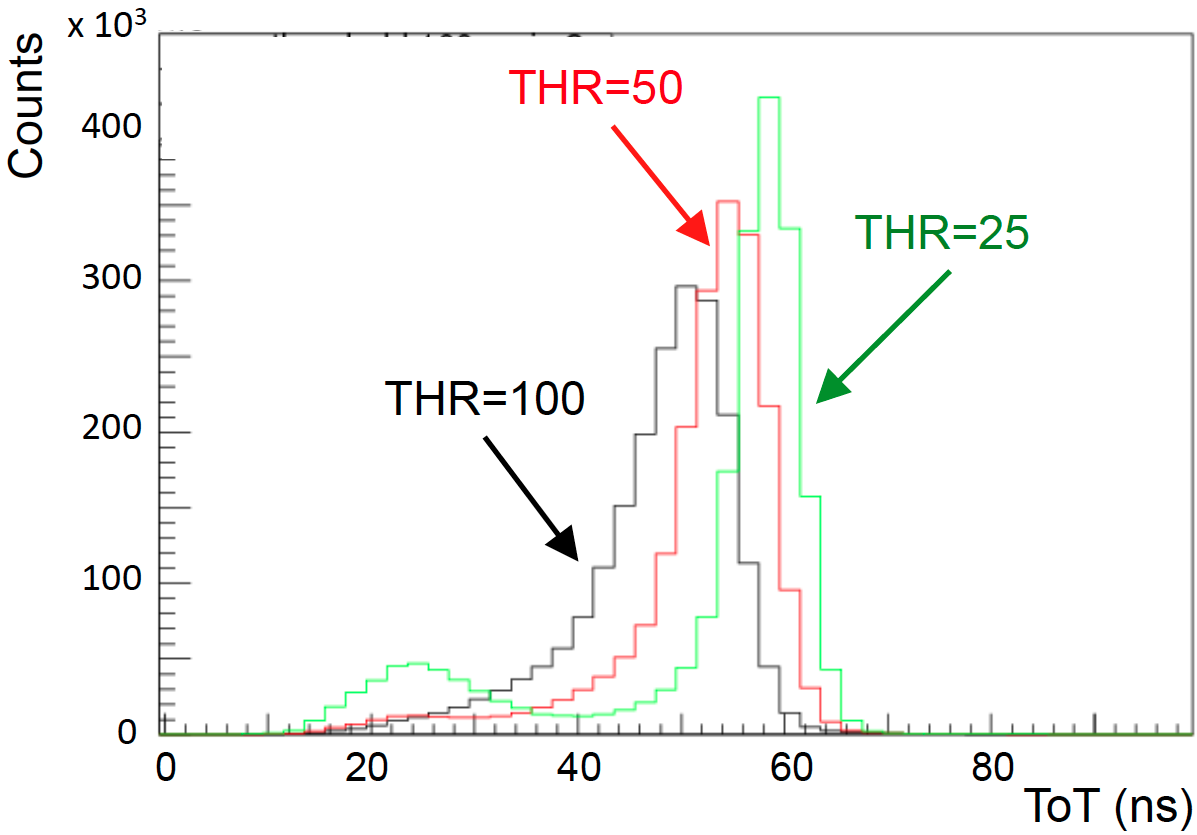
\includegraphics[width=0.95\columnwidth]{Equalize_after.png}
\end{center}
\caption{Time-over-Threshold (ToT) distributions of the RICH channels at three typical values of threshold (25, 50,
  and 100 DAC) without (top) and with (bottom) gain equalization. The saturated SPE signals generally yield ToT durations
  greater than 40~ns. When lowering the threshold weaker cross-talk signals are also recorded with ToT durations
  around 25~ns.}
\label{Fig:Equali}
\end{figure}

The MAROC preamplifier equalization gains are determined using the characterization measurements described in
Section~\ref{sec:FEtests} by tuning the average MaPMT+MAROC gain to $2.7 \times 10^6$ in all channels. The
equalization gains range from about 0.5 to 3, with an average value of 1.2. The effect of the channel-by-channel signal
equalization was verified during the engineering run by taking data at various thresholds for different MAROC gain
configurations.  Figure~\ref{Fig:Equali} shows the ToT distribution for three typical values of the threshold, on the top
for all channels without amplification (nominal MAROC gain of 1) and on the bottom after equalization. After equalization,
the ToT distribution of saturated SPE signals is narrower than with unitary gains.  With typical ToT values larger than
40~ns, the signal region is also clearly separated from the cross-talk signals whose ToT values are distributed around
25~ns.

After these tests, the common discriminator thresholds were set to +25 DAC units above the average MaPMT
pedestal position, a level that corresponds to a small fraction of the average SPE amplitude.

\begin{figure}[t]
\begin{center}
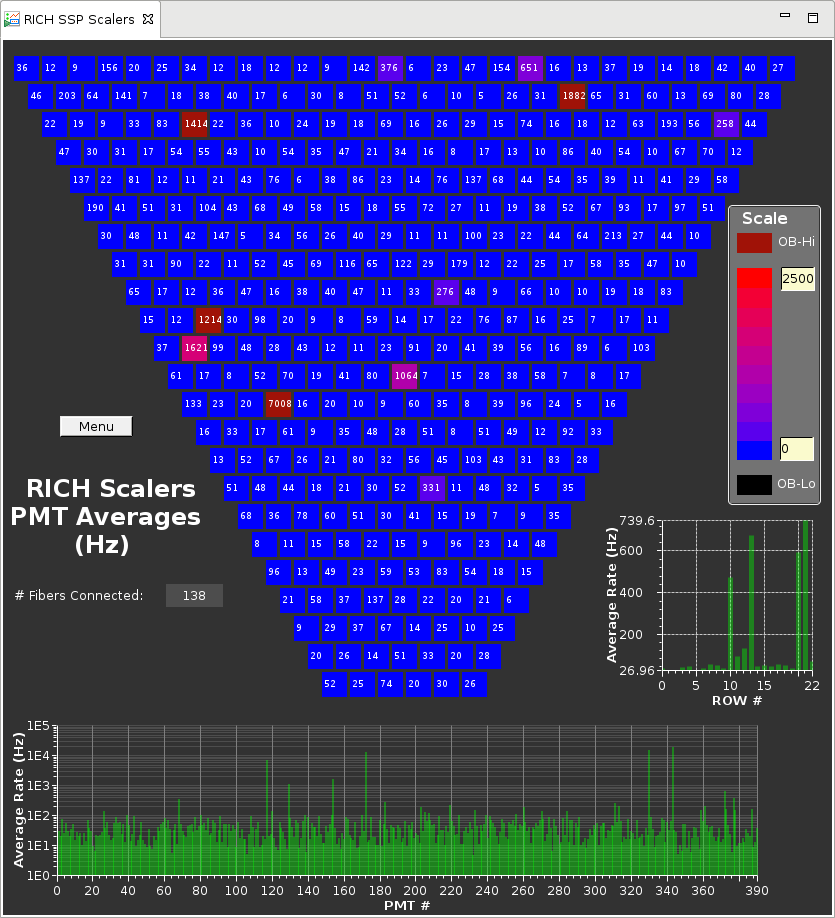
\includegraphics[width=0.7\columnwidth]{Scalers_BeamOff.png}
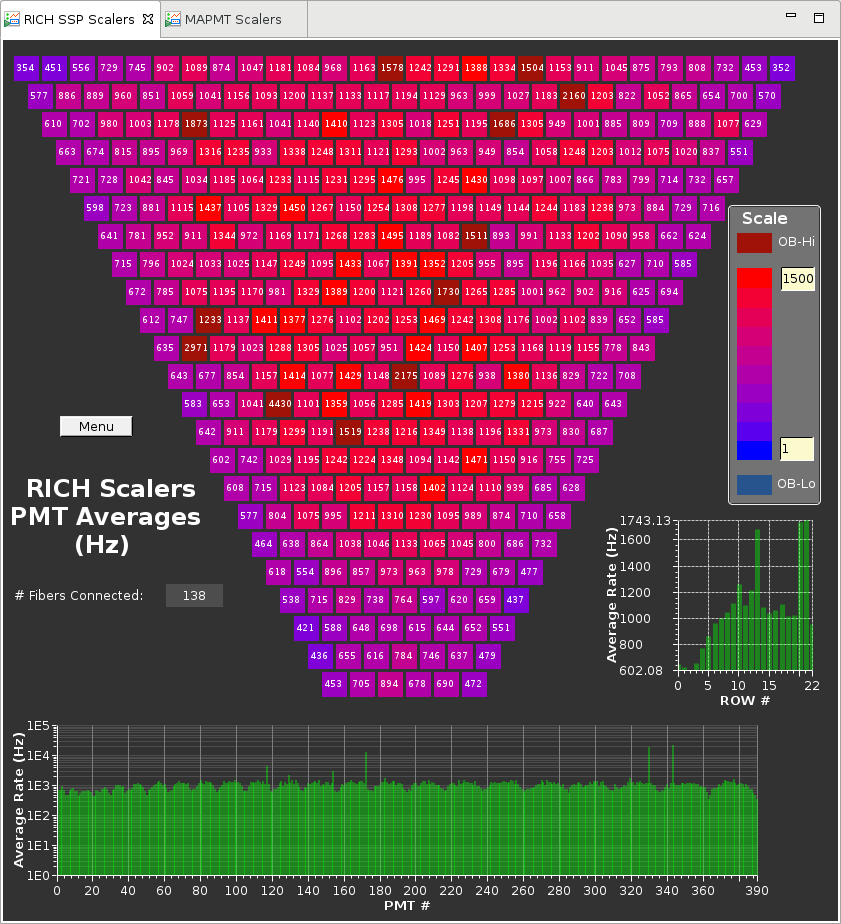
\includegraphics[width=0.7\columnwidth]{Scalers_BeamOn.png}
\end{center}
\caption{The average count rates (in Hz) over 64 pixels for each MaPMT during data taking. Top: without beam on
  target, Bottom: with beam.}
\label{fig:Online_Scalers}
\end{figure}

%------------------------------------------------
\section{RICH Slow Control and Interlocks}
%------------------------------------------------
\label{sec:SlowControl}

The RICH slow controls are based on Experimental Physics Industrial Control System (EPICS)~\cite{Ref:EPICS}. It
includes EPICS input-output controllers (IOCs) interfacing with different types of hardware via communication
protocols and over 25k RICH process variables (PVs). The controls system monitors many aspects of the RICH
detector, such as the scaler rates of all 25k Hamamatsu MaPMT pixels, the FPGA temperatures of each readout
board, the HV and LV power supplies, the LV and current consumption of each readout unit, the gas system, and
the temperature and humidity of the electronics panel volume and detector volume. For the Graphical User Interface
(GUI), the Control Systems Studio (CS-Studio), 
%developed at Oak Ridge National Laboratory.
%\cite{Ref:css-website}.   
%CS-Studio is 
an Eclipse-based suite of tools for developing and monitoring large-scale control systems, is used. 
%Fig.~\ref{Fig:RICH_overview} shows the main GUI interface of the RICH slow control. This GUI allows to have direct access to the control of the HV and LV power supply, hardware and software interlocks, as well as to launch the control  of the FPGA temperatures for each readout unit (see Fig.~~\ref{fig:Online_FPGATempMap}) and the average over 64 pixels count rates (in Hz) for each MaPMTs (see Fig.~~\ref{fig:Online_Scalers}).
 
%\begin{figure}[t]
%\begin{center}
%\includegraphics[width=0.8\columnwidth]{RICH_overview.png}
%\end{center}
%\caption{(Color online) The main GUI interface of the RICH slow control.}
%\label{Fig:RICH_overview}
%\end{figure}

The quality of the data is monitored by scaler and TDC plots. Figure~\ref{fig:Online_Scalers} shows the average 
MaPMT rate measured by the scaler readout system when the beam is off (top plot) and when the beam is on
(bottom plot). In the top plot, the few MaPMTs with hot pixels where the dark rate is substantially higher than the
average can easily be seen. The bottom plot shows that when the beam is on the rate is always dominated by physics
events. Figure~\ref{fig:Online_TDC} shows the occupancy plots from the TDC readout. The top plot shows the
occupancy per channel, and the center and bottom plots show the distributions of the leading and trailing edge times
per MaPMT, respectively. All of these plots are used during the data taking to identify possible malfunctioning channels
and, eventually, restore them through a recovery procedure.
%(see recovery button in Fig:\ref{Fig:RICH_overview}). 

\begin{figure}[t]
\begin{center}
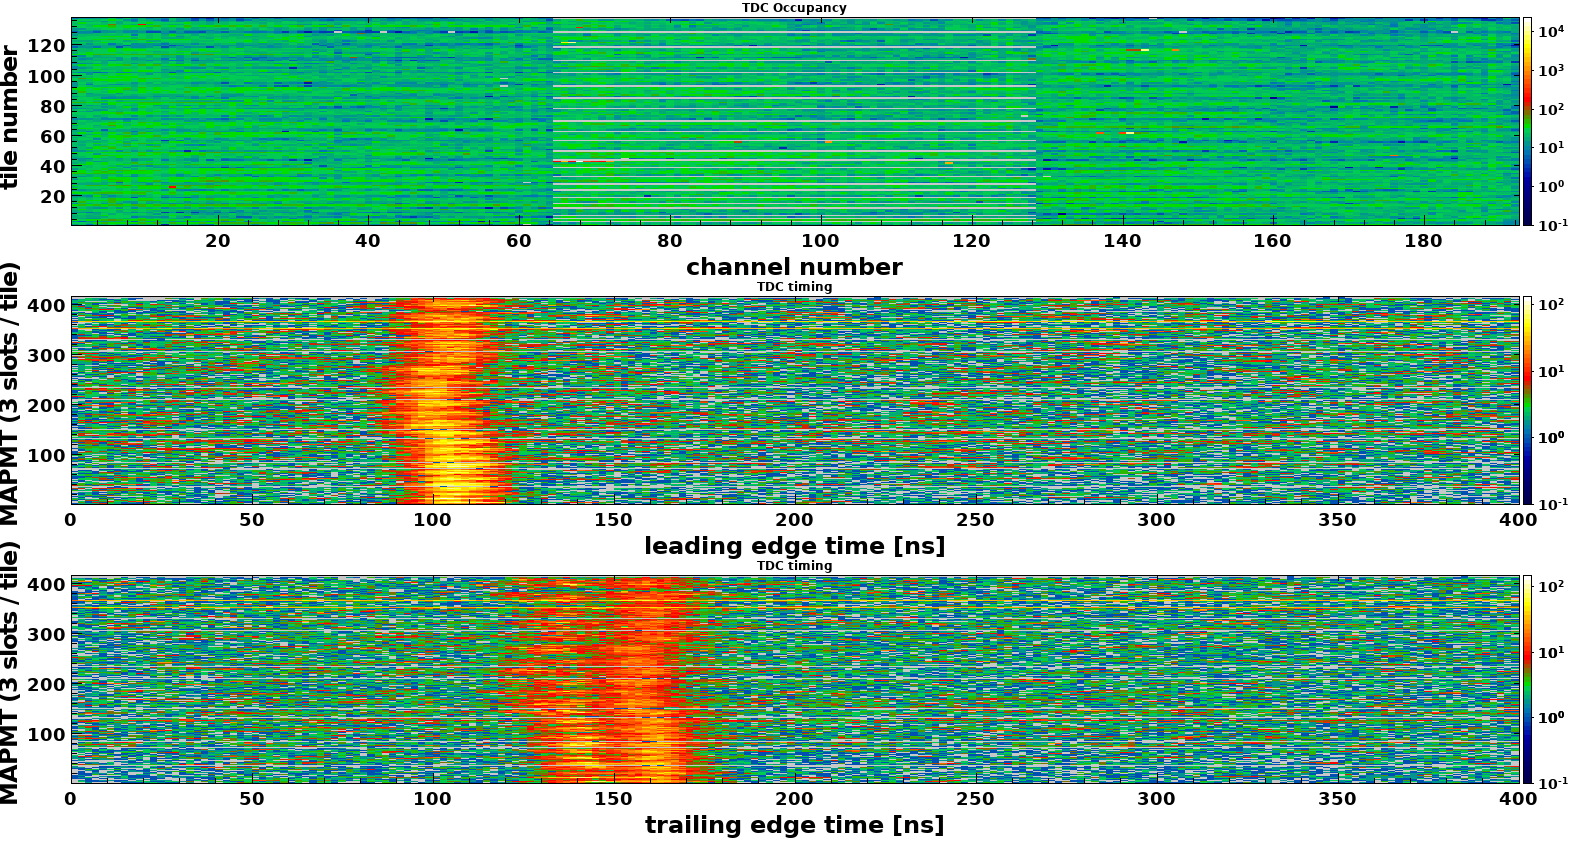
\includegraphics[width=1.0\columnwidth]{TDC_BeamOn.png}
\end{center}
\caption{Online monitor plots of the TDC occupancy with beam on. From top to bottom: channel occupancy in terms of the
  tile vs. channel number; leading edge time distributions per MaPMT; trailing edge time distribution per MaPMT.}
\label{fig:Online_TDC}
\end{figure}

%%%%%%%  cRio
%\begin{figure}
%\begin{center}
%\includegraphics[width=1.0\columnwidth]{cRio_crate.png}
%\end{center}
%\caption {(Color online) cRIO system inside National Instruments chassis.}
%\label{Fig:cRio_crate}
%\end{figure}

%\begin{figure}
%\begin{center}
%\includegraphics[width=0.7\columnwidth]{RICH_hardware_interl%ock.png}
%\end{center}
%\caption{(Color online) RICH hardware interlock GUI.}
%\label{Fig:RICH_hardware_interlock}
%\end{figure}

%\begin{figure}
%\begin{center}
%\includegraphics[width=0.7\columnwidth]{cRio_schematics.png}
%\end{center}
%\caption{(Color online) RICH control, monitoring, and interlock system, using
%both a cRIO and EPICS.}
%\label{Fig:cRio_schematics}
%\end{figure}

The slow controls and monitoring of the RICH detector is enforced by the hardware interlock system based on the
National Instruments CompactRIO (cRIO)~\cite{Ref:cRIO}.
%The cRIO system’s hardware architecture, 
%Fig.~\ref{Fig:cRio_crate}, 
%consists of a chassis, I/O and relay modules, power supply, a reconfigurable FPGA, and an embedded controller, which can be programmed in LabVIEW, C/C++, or Java.  The cRIO GUI interface is presented in Fig.\ref{Fig:RICH_hardware_interlock}.
%A cRIO system obtains signals via hardwired connections to detector sensors and instrumentation, which in turn are hardwired to the detector (red lines). cRIO systems was configured to send process variables to EPICS via Ethernet (black lines), using the standard cRIO/EPICS interface. cRIO systems do not require network connectivity. It is this feature that makes cRIO control, monitoring, and interlock systems invaluable. 
The cRIO system monitors the following parameters:
\begin{itemize}
\item Temperature and humidity in 16 locations of the detector volume;
\item Temperature and humidity in 16 locations of the electronics panel;
\item Air tank pressure;
\item Air and nitrogen flow. 
\end{itemize}

\begin{figure}[t]
\begin{center}
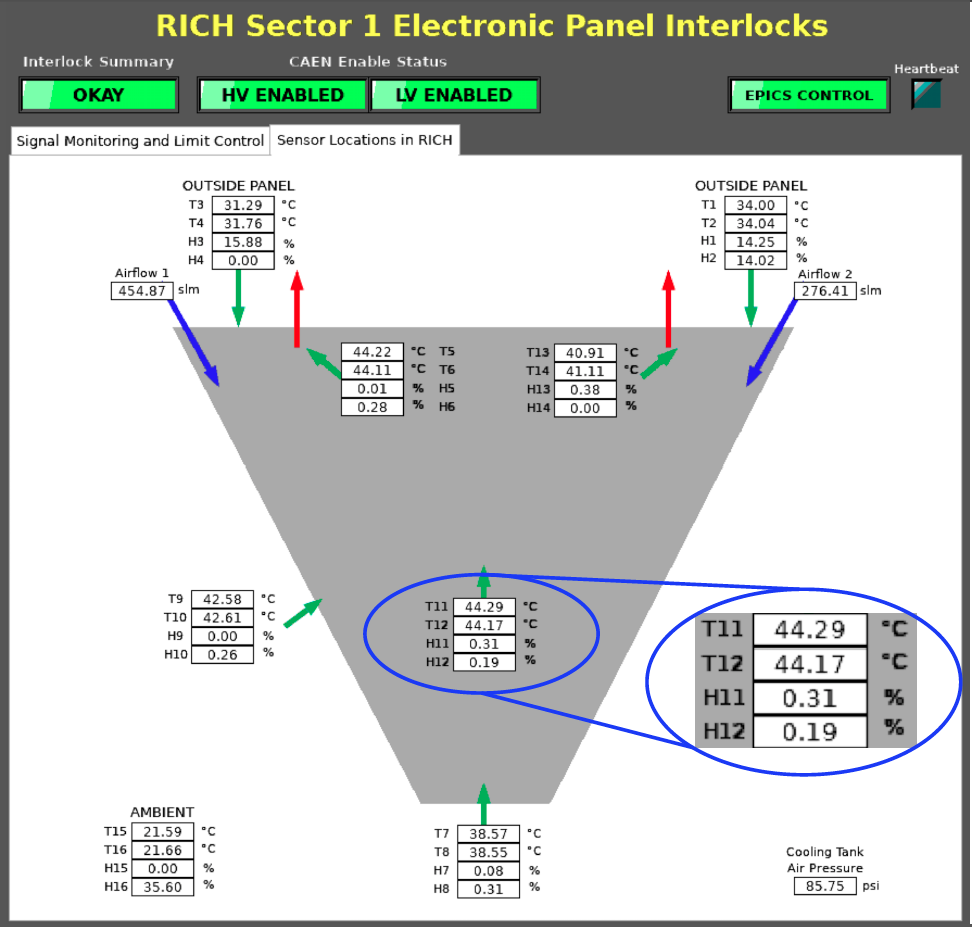
\includegraphics[width=0.9\columnwidth]{RICH_sensors_e_panel2.png}
\end{center}
\caption{Location of the temperature, humidity, and gas flow meters in the electronics panel.}
\label{Fig:RICH_sensors_e_panel}
\end{figure}

\begin{figure}[t]
\begin{center}
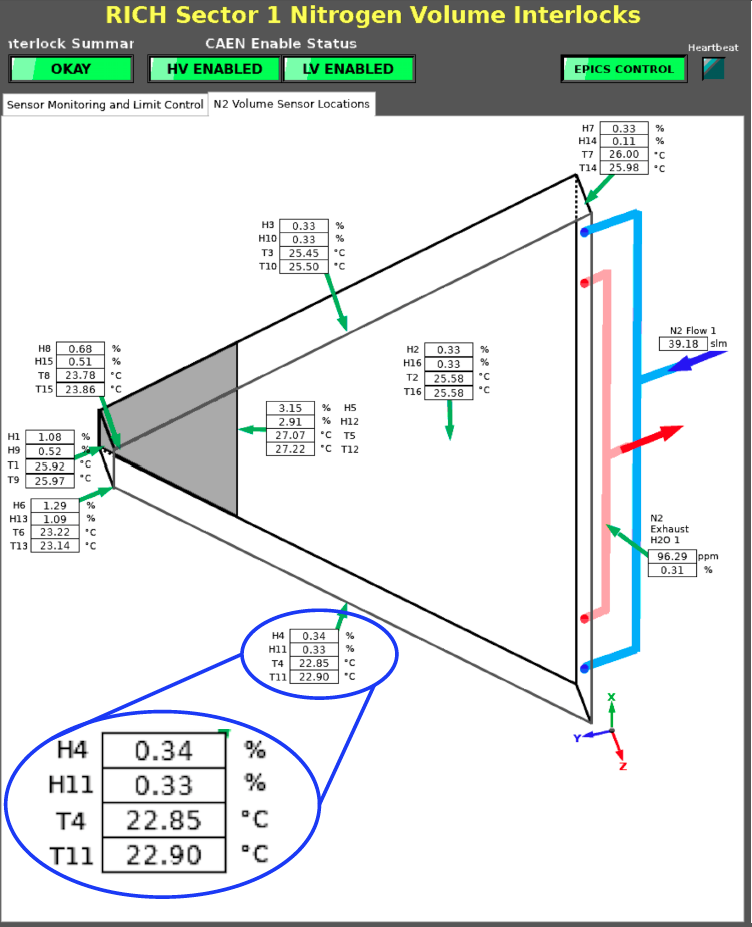
\includegraphics[width=0.8\columnwidth]{RICH_sensors_nitrogen2.png}
\end{center}
\caption{Location of the temperature, humidity, and gas flow meters in the nitrogen volume.}
\label{Fig:RICH_sensors_nitrogen}
\end{figure}

\begin{figure}[t]
\begin{center}
\includegraphics[width=0.7\columnwidth]{FPGATempMap.png}
\end{center}
\caption{Slow controls display: Map of the temperatures measured on the FPGA chips.}
\label{fig:Online_FPGATempMap}
\end{figure}

The locations of the temperature and humidity sensors, and the air and nitrogen flow meters inside the electronics
panel and nitrogen volume are shown in Figs.~\ref{Fig:RICH_sensors_e_panel} and \ref{Fig:RICH_sensors_nitrogen},
respectively. The inner temperature of the electronics panel ranges between $\rm 38.5^\circ$C and $\rm 44.5^\circ$C
moving from the bottom towards the top of the module, whereas the external temperature stays below $\rm 34.5^\circ$C,
in accordance with the requirement to not drive the FTOF system above $\rm 40^\circ$C. The relative humidity is below
0.5\%. In the nitrogen volume, the temperature ranges between $\rm 23^\circ$C and $\rm 27^\circ$C. The relative
humidity is below 1.3\% except in the central point close to the spherical mirror pivot, where it reaches a 3\% value.

The signal levels are controlled by setting limits.  If the temperatures, air flow, or air pressure go out of limits, the
HV and LV are powered off, i.e. interlocked. In case the humidity or the nitrogen flow are out of limits, an alarm signal
is generated.

Important safety parameters of the RICH detector are: the temperature of the front-end electronics, the nitrogen
flow, and the RICH internal relative humidity. Figure~\ref{fig:Online_FPGATempMap} presents the map of the
temperatures of the front-end electronics.
%and Fig.~\ref{fig:Online_EPanelTempStrip} presents the strip charts.
Typical temperature values are around 65$^\circ$C on the FPGA chips and 40$^\circ$C in the detector volume.
%The slow control interlock monitors the FPGA temperatures all the time and switches off the HV and LV power supply in case the maximum temperature exceeds the programmable limit (see Fig.~\ref{Fig:RICH_overview}).  
The safety temperature limits are 85$^\circ$C for the FPGAs, 80$^\circ$C for the optical fiber cables, and 40$^\circ$C
for the temperature on the FTOF detector, which is about 10~cm away from the RICH. Therefore, the maximum
allowed temperature was set to 75$^\circ$C on the FPGA and to 45$^\circ$C inside the electronics panel.

%\begin{figure}[t]
%\begin{center}
%\includegraphics[width=1.0\columnwidth]{EpanelTempStrip.png}
%\end{center}
%\caption{Slow control display: time evolution of the temperatures measured by the probes inside the electronic panels and in the Hall-B room (probe 16). The electronics was turned on at the time $t \approx 150$ min.}
%\label{fig:Online_EPanelTempStrip}
%\end{figure}

The nitrogen flow and the RICH internal relative humidity are measured by several probes installed inside the
detector.
%A strip chart of the reported humidity spanning a time interval of several days is shown in Fig.\ref{fig:Online_Humidity}.
An alarm is sent out in case the humidity exceeds 5\% or in case the nitrogen flow drops below the normal value. 
In the latter case, the backup system starts working to restore the normal flow level and to ensure safe humidity
conditions. During RICH operation, the humidity level has proven to be very stable with time.

%\begin{figure}[t]
%\begin{center}
%\includegraphics[width=1.0\columnwidth]{HumidityStrip.png}
%\end{center}
%\caption{Slow control display: time evolution of the relative humidity measured inside the RICH vessel over a time span of several days.}
%\label{fig:Online_Humidity}
%\end{figure}

%------------------------------------------------
\section{RICH Event Reconstruction}
%------------------------------------------------
\label{sec:RICHReco}

The RICH reconstruction is organized in four steps.
%In the first step, the spatial and time information of each hit is reconstructed taking into account known spatial misalignment and time calibration corrections. If more than 3 hits are found around a local maximum, they are grouped into a RICH cluster. A cluster is typically created by a charged particle producing Cherenkov light in the MaPMT window or ionization in the sensor dynode structure. The time of the cluster is taken to be equal to the time of the local maximum, while its spatial coordinates are calculated as a weighted average over all the hits with their ToT value as weight. If a sole hit is found close to a local maximum, with an amplitude lower than 80\% of that maximum, the hit is flagged as possible cross-talk. The hit should be within a 3$\times$3 MaPMT pixel matrix (nonet) centered on the maximum, or on a MAROC input adjacent to the maximum, to be flagged as optical or electrical cross-talk, respectively. This selection rejects about 87\% of the cross-talks, see Fig.~\ref{Fig:Xtalk}. A further reduction of the leftover cross-talk contamination, at the level of 2.7\% of the signal, would be only possible with a time versus amplitude analysis, see Fig.~\ref{Fig:Spurious}. The cross-talk selection also removes a small 0.8\% fraction of true Cherenkov signals. Those correspond to MaPMT discharges that undergo incomplete dynode multiplication, while being by chance close in space to an independent Cherenkov signal. Hits flagged as cross-talks are not considered further in the RICH reconstruction.
In the first step, the spatial and time information of each hit in the MaPMTs is corrected by the spatial misalignment
and time calibration parameters. The hits are ordered as a function of their ToT value, as this reflects the
corresponding amplitude (released charge). A 3$\times$3 MaPMT pixel matrix centered around a local maximum, i.e.
the hit with the highest local ToT, is called a nonet. If more than 3 hits are found in the same nonet they are grouped
into a RICH cluster. A cluster is typically created by a charged particle producing Cherenkov light in the MaPMT
window or ionization in the sensor dynode structure. 
%The time of the cluster is taken to be equal to the time of the local maximum, while its spatial coordinates are calculated as a weighted average over all the hits with their ToT value as weight. 
If a sole hit is found close to a local maximum with a ToT lower than 80\% of that maximum, the hit is flagged as
possible cross-talk. Hits belonging to the same nonet of the local maximum are flagged as optical cross-talk, while hits
readout by an electronics channel adjacent to the maximum hit in the MAROC chip are flagged as electrical
cross-talk. Note that the readout circuit routing has been designed to connect anodes close in space to non-adjacent
MAROC3 inputs. The above selection rejects about 87\% of the cross-talk hits, as can be seen in Fig.~\ref{Fig:Xtalk}.
In the figure, the ToT distribution of the recorded RICH hits (black solid line) is shown together with the
distributions of the hits identified as optical (magenta dash-dotted line) or electrical (green dashed line) cross-talk. The
shoulders on the right of the cross-talk peaks are likely due to signal discharges wrongly identified as cross-talk.
The hits selected for further analysis are highlighted by the dotted (blue) histogram. The excess at low ToT values
indicates a residual contamination of unidentified cross-talk. The leftover cross-talk contamination, at the level of
2.7\% of the signal, can be further reduced only with a time versus amplitude analysis, see Section~\ref{sec:TimeCalib}.
The cross-talk selection also removes a small (0.8\% fraction) of true Cherenkov signals. Those correspond to MaPMT
discharges that undergo incomplete dynode multiplication, while being by chance close in space to another Cherenkov signal.
Hits flagged as cross-talk are not considered further in the RICH reconstruction.

\begin{figure}[t]
\begin{center}
\includegraphics[width=1.0\columnwidth]{xtalk.png}
\end{center}
\caption{ToT distribution of the recorded RICH hits (black solid line) together with the optical (magenta dash-dotted line)
  and electrical (green dashed line) cross-talk distributions.  The hits selected for further analysis are highlighted by the
  blue dotted histogram. }
\label{Fig:Xtalk}
\end{figure}

%In the second step, RICH clusters are associated with the CLAS12 tracks if a match in space is found, i.e. the extrapolated impact point of the track into the \MaPMT plane is closer than 10 cm to the cluster center. Matched clusters allow a precise study of the \MaPMT detector position and orientation relative to the CLAS12 tracking system, see Fig.~\ref{Fig:DCmatch}.

The second step consists in finding the spatial match between the RICH clusters and the CLAS12 charged particle tracks. This requires
that the extrapolated impact point of the track on the MaPMT plane is within 10~cm of the cluster center. The latter
is calculated as a weighted average - with the ToT value as the weight - of the spatial coordinates of all the hits in the
cluster. Matched clusters allow a precise study of the MaPMT detector position and orientation relative to the CLAS12
tracking system. This is shown in Fig.~\ref{Fig:DCmatch}, where the distance between the RICH clusters and the matched 
drift chamber tracks~\cite{REF:dc-nim} divided by the pixel spatial RMS, (a sort of $\chi^2$ distribution), is reported. The black
distribution is before and the red one is after the alignment procedure.

\begin{figure}[t]
\begin{center}
\includegraphics[width=1.0\columnwidth]{ckmaca.png}
\end{center}
\caption{RICH matching $\chi^2$, defined as the distance between the RICH clusters and the matched drift chamber tracks divided by the
  pixel spatial RMS. The black distribution is before and the red one is after the alignment procedure.}
\label{Fig:DCmatch}
\end{figure}

\begin{figure}[t]
\begin{center}
\includegraphics[width=1.0\columnwidth]{Tracking_time.png}
\end{center}
%\caption{The photon detection time as measured by the RICH can be compared to the more precise time extrapolated by the CLAS12 spectrometer. The latter is defined as the event start time plus the flight-times of the hadron from the interaction point to the radiator center, and of the ray-traced photon within the RICH volume. Any systematic difference emerging as the average over several events provides a mean of calibration for the RICH time. After calibration, a time coincidence within the event can be used to validate the single photon reconstructed path and emission point.}
\caption{The RICH photon detection time as measured by the  CLAS12 spectrometer. It is defined as the event start
  time plus the flight-times of the hadron from the interaction point to the radiator center, and of the ray-traced
  photon within the RICH volume.}
\label{Fig:Traced_Time}
\end{figure}

The third step is the core of the RICH reconstruction~\cite{recon-nim}. For each hit in the MaPMT plane, an
estimate of the corresponding Cherenkov angle is derived by ray-tracing the photon path inside the RICH volume
taking into account possible reflections. This is done in turn for each charged particle traced through the RICH, with
the photon emission point assumed to be the middle point of the particle path inside the aerogel radiator. In the fourth
step, a particle identification algorithm is applied using an event-based likelihood of the reconstructed Cherenkov
angles and times.

%-----------------------------------------------
\section{Time Calibration and Resolution}
%-----------------------------------------------
\label{sec:TimeCalib}

\begin{figure}[t]
\begin{center}
\includegraphics[width=0.85\columnwidth]{dt_vs_anode_nocor.png}
\includegraphics[width=0.85\columnwidth]{dt_vs_dur_nocor.png}
\end{center}
\caption{Top plot: distribution of the time difference $\Delta T$ between the measured RICH and calculated CLAS12
  times as a function of the RICH readout channel. Bottom plot: cumulative distribution of the time difference
  $\Delta T$ as a function of the hit duration time (ToT).}
\label{fig:Time_uncorr}
\end{figure}
The time information of the RICH hits is provided by the leading edge time $T_1$ measured by the TDC implemented
into the FPGA board with a 1~ns precision. In-time photon hits are selected by comparing their $T_1$ with the time
$T_{calc}$ computed using the CLAS12 information (see Fig.~\ref{Fig:Traced_Time}). $T_{calc}$ comprises the event
start time, the charged track path and flight time provided by the tracking system, and the Cherenkov photon path
reconstructed inside the RICH as explained in Ref.~\cite{recon-nim}. Being based on the precise Forward Time-of-Flight
system~\cite{REF:ftof-nim} and the accelerator RF frequency, the CLAS12 computed time features a time resolution on the order of 100~ps,
significantly better than RICH. The CLAS12 computed time can therefore be used as a reference for the RICH time calibration.
%Any systematic difference emerging as the average over several events provides a mean of calibration for the RICH time. After calibration, a time coincidence within the event can be used to validate the single photon reconstructed path and emission point.

With respect to the expected time resolution, significant channel-by-channel variations are found in the difference
between the measured and the calculated times as shown in the top plot of Fig.~\ref{fig:Time_uncorr}, where the
distribution of $\Delta T=T_1-T_{calc}$ as a function of the channel number is shown. These variations are introduced
by the readout chain, with the biggest contribution coming from the average length of the 3 optical DAQ fiber trunks and
from the specific length of the various fibers in each trunk. Smaller variations among the individual channels of one
board can also occur due to the different circuit routing and components. An additional overall time constant is
expected from the relative calibration of the RICH with respect to the rest of the CLAS12 detectors.

A broadening of the $\Delta T$ distributions is due to the time walk, i.e. the dependence of the trailing edge time
on the amplitude of the input signal. Since the MAROC3 readout mostly works in the saturated regime already
at the SPE level, this effect is expected to be relevant for small amplitude signals, as can be seen from the bottom
plot of Fig.~\ref{fig:Time_uncorr}. Saturated signals have typical ToT values on the order of 60~ns, while small
amplitude signals are expected to be discriminated up to several ns later. The vertical band at ToT $\approx$60~ns
comprises a distribution of random-time \MaPMT dark counts and off-time beam bunches. The independent excess
around ToT $\approx$25~ns signals a residual contamination of cross-talk pulses anticipated in Section~\ref{sec:RICHReco}.

%a 4 ns periodic structure corresponding to wrong beam bunches.


A two step calibration procedure was implemented in order to align the time measured of all RICH readout
channels with the expected (calculated) one. The current version of the software uses electrons and charged pions
identified in CLAS12 with momenta larger than 2.5~GeV and Cherenkov photons reconstructed in the RICH with
no reflections on the mirrors.

The first step of the procedure consists in the evaluation of the 25024 time offset corrections. The values of
$\Delta T$ are plotted for each channel and the position of the maximum is taken as the time offset for that
channel. The top plot of Fig.~\ref{fig:Toffset} shows a typical $\Delta T$ distribution, with a pronounced peak, a
broad tail due to the time walk, and a small enhancement above $\approx$10~ns most likely due to residual cross-talk
hits. The vertical line indicates the adopted value for the time offset correction. The bottom plot of
Fig.~\ref{fig:Toffset} shows a typical map of the time offsets. Three regions of comparable values are highlighted,
corresponding to the tiles connected to the 3 optical fiber trunks, on top of smaller channel-by-channel variations.

\begin{figure}[t]
\begin{center}
\includegraphics[width=0.9\columnwidth]{Toffset_ch2913.png}
%\includegraphics[width=0.9\columnwidth]{ToffsetMap.png}
\includegraphics[width=0.95\columnwidth]{Offset_map.png}
\end{center}
\caption{Top plot: $\Delta T$ distribution for one readout channel; the red line indicates the time offset value.
  Bottom plot: typical map of the time offsets.}
\label{fig:Toffset}
\end{figure}

\begin{figure}[t]
\begin{center}
\includegraphics[width=1.0\columnwidth]{time_walk_fit.png}
\includegraphics[width=0.9\columnwidth]{Saturation_ToT2.png}
\end{center}
\caption{Top plot: fit of the time-walk correction for one MaPMT. Bottom plot: distribution of the ToT saturation
  values extracted from the time-walk corrections.}
\label{Fig:TimeWalk}
\end{figure}

Once the individual channels were corrected for the time offsets, the time-walk corrections were extracted from
the $\Delta T$ distribution as a function of ToT. Since the threshold level is common to all channels of one MAROC3
chip, and the amplitude equalization has been performed, one expects that the same time-walk correction should work
for all channels of one MaPMT. This was verified by comparing plots like the one shown in the bottom plot of
Fig.~\ref{fig:Time_uncorr} for all channels of the MaPMTs. A set of 391 time-walk correction functions, one
per MaPMT, is therefore extracted by fitting the dependence of $\Delta T$ as a function of ToT, as shown in the
top plot of Fig.~\ref{Fig:TimeWalk}. The dependence is fit with two lines, one for the saturated regime and
one for the linear region. The free parameters of the fit are the two slopes, the ToT value where the two lines cross,
i.e. the saturation ToT, and the $\Delta T$ at zero ToT. The data show small deviations from the linear behavior.
However, such a simple functional form was adopted to minimize the probability of fit failure (having to deal with
several hundreds of fits) and because it was proven to be enough to achieve time resolutions that meet the
specifications. In the bottom plot of Fig.~\ref{Fig:TimeWalk}, a typical distribution of the saturation ToT values
obtained from the fit is shown. The average value is around 57~ns with small variation from MaPMT to MaPMT.

\begin{figure}[t]
\begin{center}
\includegraphics[width=0.9\columnwidth]{dt_vs_anode_cor.png}
\includegraphics[width=0.9\columnwidth]{dt_vs_dur_cor.png}
\end{center}
\caption{Distribution of the time difference \dT between the measured RICH and extrapolated CLAS12 times after
  the time calibration. On the top as a function of the readout channel; on bottom as a function of the signal amplitude ToT.}
\label{Fig:DT_corr}
\end{figure}

\begin{figure}[h]
\begin{center}
\includegraphics[width=0.9\columnwidth]{Calibration_allch.png}
\end{center}
\caption{Typical \dT distribution before (black) and after (blue) the time-walk correction for all the RICH pixels.
The red line is a Gaussian fit of the corrected distribution, with a global width $\sigma$=0.66~ns}
\label{Fig:ResoTime}
\end{figure}

\onecolumn
\begin{figure}[t]
\begin{center}
\includegraphics[width=0.9\columnwidth]{Event_21488.png}
\end{center}
\caption{Example of a reconstructed RICH event with only direct photons.} 
\label{Fig:Event1}
\end{figure}

\begin{figure}[t]
\begin{center}
\includegraphics[width=0.9\columnwidth]{Event_13051.png}
\end{center}
\caption{Example of a reconstructed RICH event with a partial ring reflected by the lateral flat mirror.}
\label{Fig:Event2}
\end{figure}

\begin{figure}[t]
\begin{center}
\includegraphics[width=0.9\columnwidth]{Event_11846.png}
\end{center}
\caption{Example of a reconstructed RICH event with photons reflected by all the lateral mirrors.} 
\label{Fig:Event3}
\end{figure}

\begin{figure}[t]
\begin{center}
\includegraphics[width=0.9\columnwidth]{Event_20155.png}
\end{center}
\caption{Example of a reconstructed RICH event with a partial ring reflected back by the spherical mirror and
  passing twice the aerogel layer.}
\label{Fig:Event4}
\end{figure}

\twocolumn

After calibration, the corrected $\Delta T$ distribution is centered at zero for all channels, see
Fig.~\ref{Fig:DT_corr}. As a consequence, a few ns time coincidence can be applied to remove the spurious hits. As
shown in the bottom panel of Fig.~\ref{Fig:DT_corr}, the cross-talk hits at ToT $\approx$25~ns and the 4~ns
sub-structure of the off-time beam bunches at ToT $\approx$60~ns become clearly visible. A typical \dT
distribution is shown for one MaPMT in Fig.~\ref{Fig:ResoTime}, where the red and black histograms show the
$\Delta T$ values before and after the correction, respectively. The red curve is a Gaussian fit of the
corrected distribution.
%The distribution of the $\sigma$ of the Gaussian fits of all the channels are shown in the bottom plot of the Fig. \ref{Fig:ResoTimeAll}. 
On average, we obtained a time resolution $<\sigma> \approx$0.7~ns, well below the requirement of 1~ns.

%-----------------------------------------------
\section{RICH Hadron Separation}
%-----------------------------------------------
\label{sec:HadronID}

The RICH has been designed to provide hadron identification in the 3 - 8~GeV momentum range. The most
challenging separation is between kaons and pions, as their Cherenkov angles become closer and closer with the
increase of momentum until a minimum difference of 6~mrad at 8~GeV. In addition, in this momentum range the
pion yield is more than an order of magnitude larger than for the other hadron species.

%Various event topologies are possible due to the  unconventional RICH geometry that has to fit in one of the triangular CLAS12 sectors. The hybrid optical configuration requires to work simultaneously with direct photons in proximity focusing and with reflected photons in mirror focusing geometries. In the range of interest for RICH, between 3~GeV and 8~GeV, electrons can be used as a control sample for pions as their saturated Cherenkov angles are indistinguishable. The large recorded electron statistics allows a detailed optimization of the RICH performance, still ongoing, that should take into account possible misalignments and inhomogeneities of all the optical components.

Various ring imaging topologies are possible due to the  unconventional RICH geometry. These topologies are generated
by direct photons in proximity focusing and by reflected photons in mirror focusing geometries. In the momentum
range of interest (between 3~GeV and 8~GeV), electrons can be used for a detailed optimization of the RICH
performance since, being in a saturated regime, their Cherenkov angles are indistinguishable from those of pions.
The work is still ongoing to make use of the large recorded electron statistics.

\begin{figure}[t]
\begin{center}
\includegraphics[width=1.0\columnwidth]{Tile12_rms_plot2.png}
\end{center}
\caption{RICH Cherenkov resolution before (open points) and after (solid points) a preliminary RICH alignment. The whole RICH
  detector is aligned minimizing the matching distance between RICH clusters and extrapolated drift chamber tracks. No
  possible misalignment of the single RICH component is accounted for. The distribution is for particles passing through
  one aerogel tile of 2 cm thickness (tile 12 in layer 1) and for direct photons.}
\label{Fig:Align}
\end{figure}

Examples of reconstructed RICH events are shown in Figs.~\ref{Fig:Event1} to \ref{Fig:Event4} for particles
identified as electrons by CLAS12. In each figure, the reconstructed RICH event is displayed on the left. The
ray-tracing approach allows, for each particle hypothesis, to anticipate the expected photon pattern and the associated
hits on the photodetectors, indicated by the small dots in the figures.
%In the presented cases only electrons at the measured momentum are considered (che vuoi dire con "In the presented cases only electrons at the measured momentum are considered"?). The expected photon pattern and the hits associated to the impact point of the electron track are indicated by small dots. 
The measured RICH hits are shown as open circles, whereas the reconstructed photon hits are shown as the full
circles. Direct and reflected photons are indicated in magenta and blue, respectively. A remarkable feature of the
RICH detector is the low level of spurious hits from accidentals, in-time background (i.e. Rayleigh scattering), and
dark counts. This feature is crucial for the most challenging cases: particles with high momenta close to the 8~GeV
limit that require the best resolution in Cherenkov angle, and particles pointing towards the spherical mirror whose
number of detected photons is limited by the double reflection and a second passage through the radiator. 

For each event, the details of the time and Cherenkov angle reconstruction are shown on the right. On the top panel,
the time coincidence $\Delta T$ between the RICH measured hit and the CLAS12 calculated time is displayed as a
function of the photon flight time within the RICH (photon transit time). The time coincidence $\Delta T$ should be
close to zero for any true photon path. As a consequence, a valid photon reconstruction is initially selected by
requiring $\Delta T<3$~ns, indicated by the horizontal dashed lines. The path length is represented by the photon
transit time inside the RICH, from the emission point within the aerogel to the detection point in the MaPMT plane
after all possible reflections. Photons reflected by the spherical mirror and directed back to the aerogel travel
twice the gap, with an expected significant increase of path length and a corresponding distinctive $\approx$6~ns
longer transit time. %but with a time coincidence with CLAS12 at the precision level of direct photons

In the bottom panel, the measured angles are compared to the expected distributions for different particle
hypotheses. The width of each distribution corresponds to the expected SPE angular resolution, while the average
value depends on the particle type and momentum. An acceptance range is defined from the smallest angle expected
for a proton to the largest angle expected for an electron, enlarged by three times the expected angular resolution.
For the latter, a conservative value of 6 mrad is taken for the single photon case. These limits are indicated by the
vertical dashed lines. 
%In the whole 3~GeV - 8~GeV momentum range relevant for RICH, the Cherenkov cone generated by an electron is saturated to the maximum aperture angle corresponding to the low mass of the particle and a $\rm n \approx 1.05$ refractive index (the exact value depending on the aerogel tile). 


For each reconstructed photon path an estimate of the corresponding Cherenkov angle is obtained and
histogrammed on the plot. In all cases studied, both reflected and direct photon information is consistent with
the electron hypothesis. In particular, the reconstructed reflected and direct photon paths with \dT close to
zero provide Cherenkov angle values consistent with an electron, as expected. The narrow distribution of the
measured angle values indicate that kaons can clearly be separated up to momenta greater than 6~GeV. Electrons
can be distinguished from pions only at low momenta, below 2~GeV.

Each aerogel tile presents specific features because the challenging production process, tuned to achieve the
highest transparency over a large volume, is not fully industrialized. The most important quality parameters are the
density, related to the average refractive index, homogeneity, related to the refractive index variations within the
volume, and tile bending, originated by the inner material tension and related to the surface planarity. The effect of
these features on the RICH photon reconstruction can be studied in detail using the control sample of electrons
identified by CLAS12. Given the large number of tiles and the broad range of particle directions after the CLAS12
bending magnets, such a study requires large statistics and is still ongoing. A similar approach is used for the
alignment study. Also in this case, large statistics are needed due to the numerous involved components (aerogel
layers, mirrors, and MaPMT plane) and photon path configurations. 

As a general approach, the RICH performance is studied separately for each aerogel tile.
The RICH global performance estimators are then defined by averaging the results over all the
radiator tiles. 
Despite the fact that the above studies have not yet been finalized, and only partial corrections have been
implemented so far, the preliminary SPE Cherenkov angle resolution yields typical values around 6~mrad. It is expected to improve
towards the goal value of 4.5~mrad once the corrections for the detector misalignment are implemented and the
realistic optical parameters of each aerogel tile are taken into account. As an example, the effect of a preliminary
alignment of the RICH as a whole is shown for one aerogel tile in Fig.~\ref{Fig:Align}. The
resolution is calculated as the RMS of the distribution of the average Cherenkov angles extracted for 
each single track of the electron control sample. Such averages are calculated 
over the detected photons, whose reconstructed path satisfies the time coincidence and provides an angle within the 
kinematic limits described above, associated with the track. The fit shown uses the function
$$\sigma = \sqrt{\frac{\sigma_1^2}{N}+\sigma_0^2}$$ to extract the single photon resolution $\sigma_1$ in addition to
a constant term $\sigma_0$ measuring the residual systematics due, e.g. to misalignment.
After alignment, the resolution improve towards
the design values, which are 4.5~mrad for single photon detection and 1.5~mrad for the average over all the photons 
that are associated with the control electron track. Such preliminary Cherenkov angle resolution is already sufficient for an effective hadron
separation in the goal range of momenta, from 3 to 8~GeV, as shown by Figs.~\ref{Fig:CHele} to \ref{Fig:CHhad2}.

\begin{figure}[t]
\begin{center}
\includegraphics[width=1.0\columnwidth]{Electron_PID.png}
\end{center}
\caption{RICH response for electrons as identified by CLAS12. As expected, the measured Cherenkov angle
  is saturated over the whole momentum range, from 3~GeV up to 8~GeV. The distribution is for particles passing
  through one aerogel tile of 2~cm thickness (tile 12 in layer 1) and direct photons.}
\label{Fig:CHele}
\end{figure}

\begin{figure}[t]
\begin{center}
\includegraphics[width=1.0\columnwidth]{Hadron_PID.png}
\end{center}
\caption{RICH response for non-electron particles as defined by CLAS12. The measured Cherenkov angles distribute
  around the expected values for pion, kaon, and proton hypotheses as a function of their momentum. The three hadron
  populations are separated over the whole momentum range, from 3~GeV up to 8~GeV. The distribution is for
  particles passing through one aerogel tile of 2~cm thickness (tile 12 in layer 1) and spanning the entire momentum
  range of interest for RICH.}
\label{Fig:CHhad1}
\end{figure}

\begin{figure}[t]
\begin{center}
\includegraphics[width=1.0\columnwidth]{Pslices.png}
\end{center}
\caption{RICH response for non-electron particles in slices of momentum, from 4~GeV up to 7~GeV.}
\label{Fig:CHhad2}
\end{figure}

%-------------------------------------------------------
\section{Conclusions}
%-------------------------------------------------------

A RICH detector has been designed to enhance the hadron identification capability 
at CLAS12 in the 3 to 8 GeV momentum range. It substitutes the baseline gas threshold Cherenkov detector 
in two of the CLAS12 sectors, to create a symmetric left-right setup 
optimized for running with polarized targets. The first module was
installed at the beginning of 2018, in time for the start of the experiment data 
taking. The second module is under construction and expected to be ready in 
the summer 2021, in time for the first run with polarized targets.

To efficiently cover the wanted few-GeV momentum range, the RICH employs 
innovative technological solutions. Among these are composite 
aeronautic light-materials to ensure the needed mechanical structure rigidity, 
aerogel radiators of unprecedented large volume (up to $200 \times 200 \times 30$ $\rm mm^3$) 
and high transparency ($\approx$50~mm scattering length), light 
(of the order of 1\% radiation length) mirrors made of carbon-fiber or, for
the first time in a nuclear experiment, glass-skin technology, and
high-segmented and high-packed Hamamatsu H8500 and H12700 multi-anode photomultipliers.
A compact and scalable readout electronics system has been realized for 
the detector, able to discriminate Cherenkov signals down to as small as a 1/32 fraction
of the single photon amplitude, with excellent efficiency and stability,
and a time resolution better than 1 ns.

The peculiar geometry of the CLAS12 sector suggested a innovative 
hybrid-optics solution to limit the active area to $\approx$1~m$^2$ per sector, with part of the light directly
imaged and part of the light detected after reflection from mirrors. This and the bending into
the torus field of the CLAS12 Forward Detector create a variety of
possible topologies for the particle and photons paths. 
The RICH reconstruction exploits a ray-tracing algorithm to provide a
Cherenkov angle estimation for each photon hit and hadron track in 
the event. This basic experimental information allows an independent 
development of higher-level PID algorithms with increasing sophistication.

Preliminary data analysis shows that the CLAS12 RICH is able to match the 
required time and Cherenkov angle resolutions. After calibration, each
of the 25k channels features a time resolution of the order of 0.6~ns,
better than the 1~ns specification. High momentum particles
define the most stringent requirements for the RICH performance. As the pion yield
supersedes the other particles species by an order of magnitude, a 
$4\sigma$ angle separation is required to contain the contamination 
at the percent level. At 8~GeV, this implies an angle resolution of 1.5~mrad.
Despite the fact that the detailed study of the alignment and optical performance of the various 
components is still ongoing, the detector has already demonstrated a single-photon 
angle resolution better than 5~mrad and an average number of 19 photons per charged particle
in the forward high-momentum direction, in line with the detector design specifications. This reflects in an angle resolution 
per charged particle close to the design value of 1.5~mrad and an effective hadron identification 
capability over the entire required momentum range.

%-------------------------------------------------------
\section{Acknowledgments}
%-------------------------------------------------------

%\vspace{0.2cm}
This material is based upon work supported by INFN under the MIUR priority project CLASMED, Italy and by the
U.S. Department of Energy, Office of Science, Office of Nuclear Physics under contract DE-AC05-06OR23177 and
the National Science Foundation, Award \#1615067. We thank the JLab Detector Support Group and Fast Electronics
Group, the Hall~B technical and management staff, and the INFN technical and administrative service.


%-------------------------------------------------------
\begin{thebibliography}{00}
%-------------------------------------------------------
\bibitem{REF:htcc-nim}
Y. Sharabian {\it et al.}, {\it ``The CLAS12 High Threshold Cherenkov Counter''}, 
to be published in Nucl. Inst.  and Meth. A, (2020). (see this issue)
  
\bibitem{REF:ltcc-nim}
M. Ungaro {\it et al.}, {\it ``The CLAS12 Low Threshold Cherenkov Counter''}, 
to be published in Nucl. Inst.  and Meth. A, (2020). (see this issue)

\bibitem{REF:ftof-nim}
D.S. Carman {\it et al.}, {\it ``The CLAS12 Forward Time-of-Flight System''}, 
to be published in Nucl. Inst.  and Meth. A, (2020). (see this issue)
  
\bibitem{REF:overview-nim}
V.D. Burkert {\it et al.}, {\it ``The CLAS12 Spectrometer at Jefferson Laboratory''}, 
to be published in Nucl. Inst.  and Meth. A, (2020). (see this issue)
  
\bibitem{REF:ecal-nim}
G. Asryan {\it et al.}, {\it ``The CLAS12 Forward Electromagnetic Calorimter''}, 
to be published in Nucl. Inst.  and Meth. A, (2020). (see this issue)
  
\bibitem{REF:RICH2013} 
M. Contalbrigo {\it et al.}, {\it ``The Large-Area Hybrid-optics CLAS12 RICH Detector: Tests of Innovative Components''},
Nucl. Inst. Meth. {\bf A766}, 22 (2014).

\bibitem{REF:CMA} \url{http://www.compositemirrors.com/}.

\bibitem{REF:LHCbMirrors} 
G.J. Barber {\it et al.}, {\it ``Development of Lightweight Carbon-Fiber Mirrors for the RICH 1 Detector of LHCb''},
Nucl. Inst. Meth. {\bf A593}, 624 (2008).

\bibitem{REF:ECI} \url{https://www.evaporatedcoatings.com/}.

\bibitem{REF:MediaLario} \url{http://www.media-lario.com/}.

\bibitem{REF:RICH2016mc} 
M. Contalbrigo {\it et al.}, {\it ``Aerogel mass production for the CLAS12 RICH: Novel characterization methods and optical performance''},
Nucl. Inst. Meth. {\bf A876}, 168 (2017).

\bibitem{REF:Hunt} 
E.~Aschenauer  {\it et al.}, {\it ``Optical Characterization of n = 1.03 Silica Aerogel used as Radiator in the RICH of HERMES''},
Nucl. Inst. Meth. {\bf A 440}, 338 (2000).

\bibitem{Ref:H8500} \url{https://www.hamamatsu.com/resources/pdf/etd/H8500\_H10966\_TPMH1327E.pdf}.
  
\bibitem{REF:MaPMT_test} 
R.~A. Montgomery {\it et al.}, {\it ``Multianode Photomultiplier Tube Studies for Imaging Applications''},
Nucl. Inst. Meth. {\bf A 695}, 326 (2012).

\bibitem{REF:RICH_CERN} 
S.~Anefalos~Pereira {\it et al.}, {\it ``Test of the CLAS12 RICH Large Scale Prototype in the Direct Proximity Focusing Configuration''},
Eur. Phys. J. A {\bf 52}, 23 (2016).

\bibitem{Ref:H12700} \url{https://www.hamamatsu.com/resources/pdf/etd/H12700\_TPMH1348E.pdf}.

\bibitem{MAROC3:chip} S. Blin {\it et al.}, {\it ``MAROC, a Generic Photomultiplier Readout Chip''},
IEEE Nucl. Sci. Symp. Conf. Rec. 2010, 1690 (2010).

\bibitem{daq-nim}
S. Boyarinov {\it et al.}, {\it ``The CLAS12 Data Acquisition System''}, 
to be published in Nucl. Inst. and Meth. A, (2020). (see this issue)

\bibitem{Pavel} 
Pavel Degtiarenko, {\it ``Precision Analysis of the Photomultiplier Response to Ultra Low Signals''}, 
Nucl. Inst. Meth. {\bf A872}, 1 (2017).

\bibitem{Ref:RICHElectro} 
M. Contalbrigo {\it et al.}, {\it ``Single Photon Detection with the Multi-anode CLAS12 RICH Detector''}, 
in press in Nuc. Inst. Meth. A.,
DOI:10.1016/j.nima.2019.04.077

\bibitem{Ref:EPICS} Experimental Industrial Physics Control System, https://epics-controls.org

\bibitem{Ref:cRIO} \url{https://www.jlab.org/div_dept/physics_division/dsg/notes/2016-012%20National%20Instruments%20compactRIO-based%20control,%20monitoring,%20and%20interlock%20system.pdf}

\bibitem{REF:dc-nim}
M.D. Mestayer {\it et al.}, {\it ``The CLAS12 Drift Chamber System''}, to be published in Nucl. Inst.
and Meth. A, (2020). (see this issue)

\bibitem{recon-nim}
V. Ziegler {\it et al.}, {\it ``The CLAS12 Software Framework and Event Reconstruction''}, to be published in Nucl. Inst.
and Meth. A, (2020). (see this issue)
  
\end{thebibliography}

\end{document}

%\bibitem{CLAS12:tdr} CLAS12 Technical Design Report, version 5.1 208 (2008).
%\bibitem{CLAS12:physics} J. Dudek {\it et al.}, Eur.Phys.J. {\bf A48} (2012) 187.
%\bibitem{PSHP10} H.~Avakian \etal, {\em arXiv:1202.1910v2} {\bf [hep-ex]} (2012).
%\bibitem{RICH:first} M.~Contalbrigo \etal, {\em Nucl. Inst. Meth.} {\bf A 639} (2011) 302.
%\bibitem{RICH:ElAlaoui} A.~El~Alaoui \etal, {\em Physics Procedia} {\bf 37} (2012) 773.
%\bibitem{REF:Tecnavan} \url{http://www.tecnavan.it/en/}.
%\bibitem{REF:Aerogel} R. De Leo {\it et al.}, Nucl. Inst.Meth. {\bf A 595} (2008) 19; A. Yu. Barnyakov {\it et al.}, Nucl. Instrum. Meth. {\bf A 453} (2000) 326; R. Pereira {\it et al.}, Nucl. Instrum. Meth. {\bf A 639} (2011) 37; R. Forty {\it et al.}, Nucl. Instrum. Meth. {\bf A 623} (2010) 294.
%\bibitem{REF:Belle} T. Iijima {\it et al.}, Nucl. Instrum. Meth. {\bf A 598} (2009) 138.

%\bibitem{H8500_datasheet} \url{https://www.hamamatsu.com/resources/pdf/etd/H8500_H10966_TPMH1327E.pdf}.
%\bibitem{H12700_datasheet} \url{https://www.hamamatsu.com/resources/pdf/etd/H12700_TPMH1348E.pdf}.
%\bibitem{Bellamy} E.H. Bellamy  \etal, Absolute calibration and monitoring of a spectrometric channel using a photomultiplier, Nuc. Inst. \& Meth. in Phys. Res. A \textbf{339}, 468-476 (1994).

%\bibitem{MaPMT:laser} M.~Contalbrigo \etal, {\em Nucl. Instrum. Meth.} {\bf A 787} (2015) 224.
%\bibitem{MaPMT:model} P.~Degtiarenko, arXiv:1608.07525.
%\bibitem{Ref:GlueX} F.~Barbosa \etal, {\em Nucl. Instrum. Meth.} {\bf A 876} (2017) 69.
%\bibitem{Ref:mRICH1} C.P.~Wong \etal, {\em Nucl. Instrum. Meth.} {\bf A 871} (2017) 13.
%\bibitem{Ref:eRD14} A.~Del~Dotto \etal, {\em Nucl. Instrum. Meth.} {\bf A 876} (2017) 237.
%\bibitem{Ref:H13700} \url{https://www.hamamatsu.com/resources/pdf/etd/H13700\_TPMH1370E.pdf}.
%\bibitem{Ref:MPPC} \url{https://www.hamamatsu.com/resources/pdf/ssd/s13361-3050\_series\_kapd1054e.pdf}.

 %\bibitem{Past:rich} R. De Leo \etal, {\em Nucl. Instrum. Meth.} {\bf A 595} (2008) 19;
%A.~Yu. Barnyakov \etal, {\em Nucl. Instrum. Meth.} {\bf A 453} (2000) 326;
%R. Pereira \etal, {\em Nucl. Instrum. Meth.} {\bf A 639} (2011) 37;
%R. Forty \etal, {\em Nucl. Instrum. Meth.} {\bf A 623} (2010) 294.
%\bibitem{Belle:rich} T. Iijima \etal, {\em Nucl. Instrum. Meth.} {\bf A 598} (2009) 138.
%\bibitem{budker:aerogel} A.~Yu. Barnyakov \etal, {\em Nucl. Instrum. Meth.} {\bf A 639} (2011) 225.
%\bibitem{aerogel:clarity} T. Bellunato \etal, {\em  Nucl. Instrum. Meth.} {\bf A 556} (2006) 140.
%\bibitem{prisma:milano} T. Bellunato \etal, {\em  Eur. Phys. J.} {\bf C 52} (2007) 759.
%\bibitem{aerogel:dispe} R. De Leo \etal, {\em  Nucl. Instrum. Meth.} {\bf A 457} (2001) 52.
%\bibitem{prisma:francia} Y. Sallaz-Damaz \etal, {\em Nucl. Instrum. Meth.} {\bf A 614} (2010) 184.
%\bibitem{CBM:rich} C. H$\rm \ddot{o}$hne \etal, {\em Nucl. Instrum. Meth.} {\bf A 639} (2011) 294.
%\bibitem{T9:beam} D.~J. Simon \etal, {\em CERN PS/PA Note 93-21} (1993) Revised version 4.8.93.
%\bibitem{JLab:physics} J.~Dudek \etal, {\em Eur.Phys.J.} {\bf A48} (2012) 187.
%\bibitem{clas12:rich_rich2013} M.~Contalbrigo \etal, {\em Nucl. Instrum. Meth.} {\bf A766} (2014) 22.

